%%%
%%%  LaTeX-Template fuer Buecher und Broschueren
%%%
%%%  Emil Khalisi, MPI fuer Kernphysik, Heidelberg
%%%  emil.khalisi @ mpi-hd . mpg . de
%%%  Tel.: 06221 / 516 -339
%%%
%%%  November 2012
%%%
%%%  Updated by Long Wang in November 2014
%%%  Email: longwang.astro@gmail.com
%%% 
%%% checking the editing option... 

\documentclass[11pt,twoside,a4paper]{report}

% ---------- Initialize Packages
%
%\usepackage[latin1]{inputenc}   % deutsche Tastatur
\usepackage[T1]{fontenc}        % Richtig trennen!
\usepackage{mathptmx}
%%\usepackage[german]{babel}      % ! Inkompatibel mit \usepackage{german}
% \usepackage[german]{babel}      % ! entweder [german] oder [british] !
%\usepackage{amsmath}            % Erweiterungen fuer mathematische Formeln
\usepackage{amssymb}            % weitere nuetzliche Erweiterungen
%
\usepackage{lscape}             % Landscape-Umgebung
\usepackage{longtable}          % seitenuebergreifende Tabellen
%\floatstyle{plain}
%\usepackage{rotating}
%\usepackage{eurosym}            % Laden des Euro-Symbols
%\usepackage{units}              % Einheiten und Brueche im nice-, text- und math-mode

\usepackage{eepic}
\usepackage[dvips]{epsfig}
%\usepackage{subfigure}
\usepackage{fancyhdr}

\usepackage{auto-pst-pdf}
\usepackage{url}
\usepackage{listings}
%\usepackage{pdflscape}
\usepackage{makecell}
\usepackage{float}
\usepackage{epstopdf}
\newcommand{\ff}[1]{\textcolor{red}{\bf #1}}
  \epstopdfDeclareGraphicsRule{.pdf}{png}{.png}{convert #1 \OutputFile}
\floatstyle{plain}
\newfloat{cctimes}{th}{ccc}[section]



% ---------- Paper characteristics
%
\setlength{\textwidth}{15.0cm}
\setlength{\textheight}{23.0cm}
%\addtolength{\textheight}{4cm}
%\addtolength{\textwidth}{2.6cm}
\setlength{\oddsidemargin}{0.5cm}
\setlength{\evensidemargin}{0.2cm}
\setlength{\topmargin}{-0.3cm}
%\addtolength{\columnsep}{0.4cm}
%
%%%%% Zeilenformatierung, siehe LaTeX-Begleiter, S. 51
%
%%%%% Seitenformatierung
%
\setlength{\textwidth}{15.0cm}
\setlength{\textheight}{23.0cm}
%\addtolength{\textheight}{4cm}
%\addtolength{\textwidth}{2.6cm}
\setlength{\oddsidemargin}{0.5cm}
\setlength{\evensidemargin}{0.2cm}
\setlength{\topmargin}{-0.3cm}
%\addtolength{\columnsep}{0.4cm}

%\setcounter{secnumdepth}{4}
%\setcounter{tocdepth}{1}


%%%%% Umbenennung von Section zu Chapter zwecks Layout
%
\renewcommand{\chapter}{\section}
\renewcommand{\thesection}{\arabic{section}}

%%%%%Header from booklet >Lichtph\"anomene<
%% \pagestyle{fancy}
%% \renewcommand{\subsectionmark}[1]{\markright{#1}{}}
%% \renewcommand{\sectionmark}[1]{\markboth{#1}{}}


%%%%% Seitenzahlen auf oberer Seitenlinie
%
\pagestyle{fancy}
\renewcommand{\sectionmark}[1]{\markboth{\thesection\ \, #1}{}}
\renewcommand{\subsectionmark}[1]%
                        {\markright{\thesubsection\ \, #1}{}}

%%%%% Titel des Kapitels auf oberer Seitenlinie
%
\lhead[\itshape \thepage]{\itshape \rightmark}
\rhead[\itshape \leftmark]{\itshape \thepage}
\cfoot{}


%%%%% Umbenennung >Figure< statt >Abbildung<
%
\makeatletter
\@addtoreset{figure}{section}
\renewcommand{\thefigure}{\thesection.\arabic{figure}}
\renewcommand{\@makecaption}[2]%             % >Figure<  statt  >Abbildung<
   {\small Figure {\thefigure}: #2} %    Begleiter, Ch. 6.5
%\renewcommand{\@makecaption}{\footnotesize} % Gr\"osse d. Captionschrift
%\renewcommand{\@mkboth}{\markboth{}}        %
\makeatother


\begin{document}

%Fuer Landscape- Format:
%\special{landscape}         % hinter dem \begin{document}- Befehl!
%documentclass[landscape]    % oben in den Optionen zu erg\"anzen!




% Beginn des Hauptdokumentes.
% ===========================


%%% Title pages.

% Titlepage

\thispagestyle{empty}
\tolerance=6000

\vspace{1cm}
\begin{center}
{\Huge \bf NBODY6++}\\[0.7cm]
{\Huge  Manual for the Computer Code}\\[0.5cm]
{\Large \textcolor{red}{ATTENTION, WORK IN PROGRESS!\\[0.5cm]
This manual is continously changing and updated.}} \\ 
\end{center}



\vspace{1cm}
\noindent
%
\begin{center}
{\Large Original authors:\\
Emil Khalisi, Long Wang, Rainer Spurzem$^\star$ \\[1ex]
}

{\Large Current main contributors:\\
Francesco Flammini Dotti, Kai Wu, Rainer Spurzem$^\star$ \\[1ex]
}
{\it
$^\star$Astronomisches Rechen--Institut,
M\"onchhofstr. 12--14, 69120 Heidelberg, Germany \\
$^\star$National Astronomical Observatories,  Chinese Academy of Sciences, Beijing, China\\
$^\star$Kavli Institute for Astronomy and Astrophysics,
Peking University, Beijing, China
}\\[1ex]
Contacts:\\
spurzem@ari.uni-heidelberg.de, spurzem@nao.cas.cn \\
fmfd@uni-heidelberg.de \\ Kai.Wu19@student.xjtlu.edu.cn
\end{center}



\noindent
\begin{figure}[bh]
  \centering
  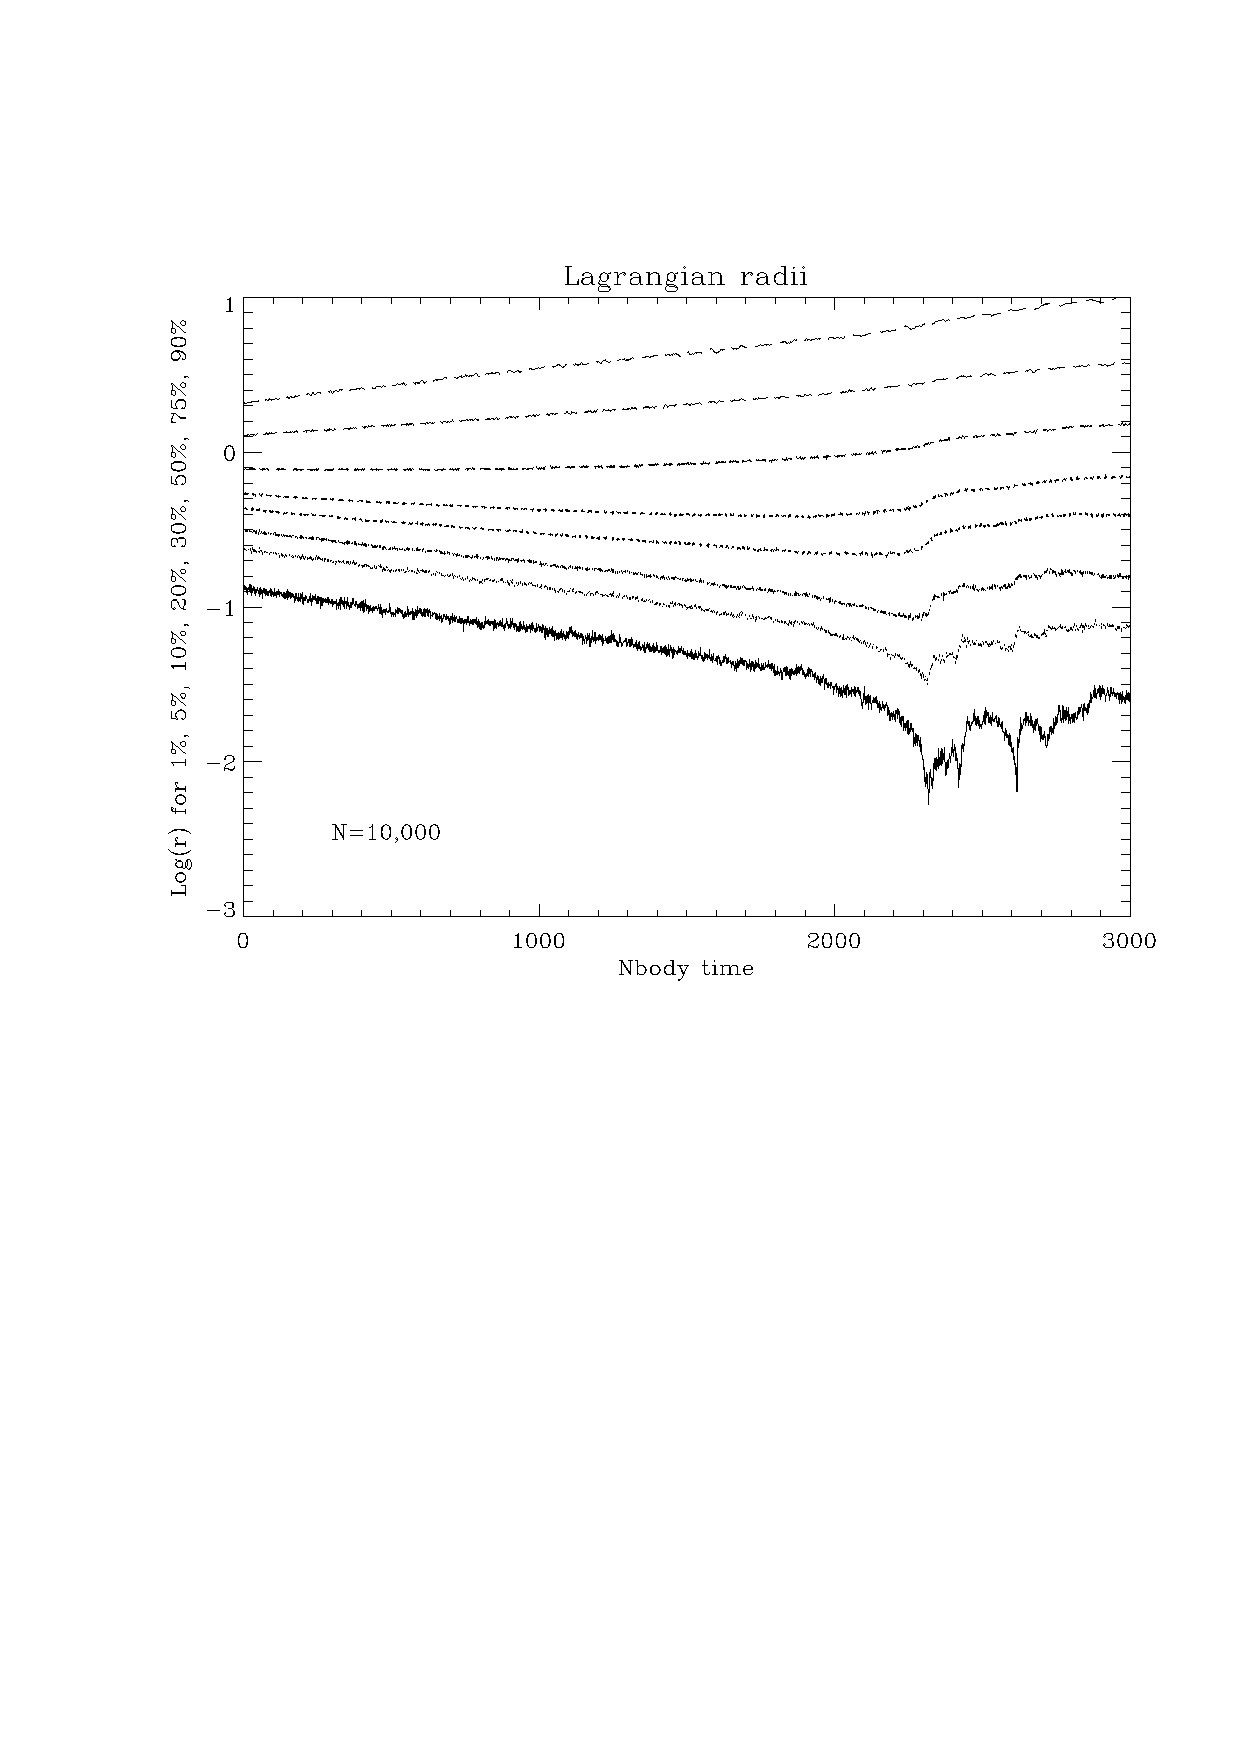
\psfig{figure=eqmass10k_03.pdf,width=0.6\textwidth}
\end{figure}

\noindent
%
\begin{center}

{\it Latest update: \today}
\end{center}
\noindent

\setlength{\headheight}{13.6pt}
\addtolength{\topmargin}{-1.59999pt}

\cleardoublepage


%%%%%  Table of contents

\thispagestyle{fancy}
\renewcommand{\contentsname}{Table of contents}
%\renewcommand{\sectionmark}[1]{\markboth{#1}{}}
\lhead[\itshape \thepage]{\itshape \contentsname}
%\rhead[\itshape \contentsname]{\itshape \thepage}
\cfoot{}

% Table of Contents
\tableofcontents

%%%%% End of introductory pages.


\clearpage

%%%%% Restore previous Header as defined in >broschure.tex<

\pagestyle{fancy}
\renewcommand{\sectionmark}[1]{\markboth{\thesection\ \, #1}{}}
\renewcommand{\subsectionmark}[1]%
                        {\markright{\thesubsection\ \, #1}{}}

\lhead[\itshape \thepage]{\itshape \rightmark}
\rhead[\itshape \leftmark]{\itshape \thepage}
\cfoot{}


 

\section{Introduction}


Gravity is an ever--present force in the Universe
and is involved into the dynamics of all kinds of bodies,
from the tiny atom to the clusters of galaxies.
At small spatial scales, its influence is covered by other
strong forces (e.g. magnetic, pressure, radiation induced),
while on the very large scale it becomes the most dominant
power.
In astrophysics, it governs the dynamical evolution of
many self--gravitating systems.
Here, we concentrate on such systems that are dominated
by mutual gravitation between particles.

The numerical star-by-star simulation of a simple cluster
containing some more than hundred thousand members still
places heavy demands on the available hard- and software.
A balance has to be found between two constraints:
On one hand the \emph{realism}, i.e.\ the input of
profound physics, inclusion of all astrophysical effects
as well as the maintenance of the accuracy of calculations;
and on the other hand, the \emph{efficiency}, i.e.\
the limitations given by the computational possibilities
and suitable codes to be finished in a reasonable time.
Many different kinds of approaches have been undertaken
to suffice both:
\begin{itemize}
\item codes based on the direct force integration
      \cite{a_85}, \cite{a_99b}, \cite{a_03}, see also:\\
      {\tt http://www.sverre.com/} ,
\item statistical models, which themselves divide into
      several subgroups
      (Fokker--Planck approximation by \cite{c_80};
      Monte--Carlo method by \cite{h_71};
      Gas models by \cite{s_94}),
\item usage of high-performance parallel computers
      \cite{s_99}, \cite{dhm_03},
\item or the construction of special hardware devoted
      for these purposes (GRAPE \cite{mtes_97},
      see also: $\;$ {\tt http://www.astrogrape.org/}
      $\;$ and $\;$ \\
      {\tt http://www.cs.rit.edu/$^{\sim}$grapecluster/} .
\end{itemize}

%All the aspects have their advantages as well as disadvantages.
The code NBODY6++GPU described in this manual is designed for
an accurate integration of many bodies
(e.g. in a star cluster, planetary system, galactic nucleus)
based on the direct integration of the Newtonian equations
of motion.
It is optimal for collisional systems, where long times of
integration and high accuracy or both are required, in order
to follow with high precision the secular evolution of the objects.

NBODY6++GPU is a descendant of the family of NBODY codes initiated
by Sverre Aarseth \cite{a_99a}, which has been extended to be
suitable for parallel computers \cite{s_99}, and further on to NBODY6++GPU by Long Wang and Rainer Spurzem \cite{Wang2015, Wang2016,Kamlah2022}. There is also a single node GPU version NBODY6GPU \cite{NA2012}. Stellar Evolution of single stars and binaries is based on Jarrod Hurley's procedures \cite{Hurley2000, Hurley2002, Hurley2005} with many recent and not so recent updates, which are summarized in \cite{Banerjee2020, Kamlah2022}.

The basic features of the code increasing the efficiency may
be considered under four separate headings:
fourth order prediction--correction method (Hermite scheme),
individual and block time--steps,
regularization of close encounters and few-body subsystems,
and a neighbour scheme (Ahmad--Cohen scheme).
We briefly describe these ideas in this booklet, while a
detailed description can be found in \cite{a_93} as well as
his book \cite{a_03}.

While NBODY6++GPU is not that different from the original NBODY6 to justify a completely new name, the user should, however, be
aware that in order to make a parallelization of regular and
irregular force computations possible at all,
some significant changes in the order of operations became 
necessary.
As a consequence, trajectories of the same initial system,
simulated by NBODY6 and NBODY6++ will diverge from each other,
due to the inherent exponential instability and deterministic
chaos in $N$-body systems.
Still one should always expect that the \emph{global}
properties are well behaved in both cases (e.g. energy
conservation).
While much effort is taken to keep NBODY6++GPU as
close as possible to to the original NBODY6 this is never 100\% the case, and the
interested should always contact Sverre Aarseth or Rainer
Spurzem if in doubt about these matters.

This manual should serve as a practical starter kit for
new students working with NBODY6++GPU.
It is not meant as a complete reference or scientific paper;
for that see the references and in particular the excellent
compendium of Aarseth's book on Gravitational
$N$-Body Simulations \cite{a_03}.

\section*{Acknowledgements}

The authors of this manual would like to express their sincere
gratitude to Sverre Aarseth, Seppo Mikkola, Jarrod Hurley, Peter Berczik, Long Wang, Albrecht Kamlah, and Manuel Arca Sedda for their continuous support and work on the code, some of them over the decades.
Also, many students and postdocs in Heidelberg, Beijing, and elsewhere
have contributed towards development, debugging and improving
the software for the benefit of the community.
%Particular thanks are due to Patrick Glaschke and Chingis Omarov.
The original booklet version was written at the Astronomisches Rechen--Institut Heidelberg under the supervision of Rainer Spurzem; now it is supported by team members of  the Silk Road Project http://silkroad.bao.ac.cn in Europe and Asia.

% sync test: overleaf-to-github verification 2026-08-20
% sync test: github-to-overleaf verification 2026-08-20

 

\section{Code versions and Download}
\label{ch:versions}

The development of the NBODY code has begun in the 1960s
\cite{a_63}, though there exist some earlier precursors
\cite{vH_60}, \cite{vH_63}.
It has set a quasi-standard for the precise direct integration
of gravitating many-body systems.
There exist several code groups (NBODY0--7, and a number of
special implementations) for different usage, some of which
are rather of historical interest.

The current code is available via \textsc{ github}\footnote{\url{https://github.com/nbody6ppgpu/Nbody6PPGPU-beijing}}. Note that a different service is provided by Long Wang, quoted here\cite{Varrietal2018}. 
The documents and input samples are included.
%In irregular intervals updates of the code are provided on
%this ftp-site.
%For those, who keep synchronicity with NBODY6++, upgrades and
%bugfixes are explained and there is usually a special README
%file detailing the changes.

The original $N$--body codes can be accessed publicly
via Sverre Aarseth's web sites at\\
\protect{\tt ftp://ftp.ast.cam.ac.uk/pub/sverre/} $\;$ and  $\;$
\protect{\tt http://www.sverre.com/} .

Special branches under our \textsc{ github} are in preparation for nuclear star clusters with central supermassive star accreting black hole and an optional accretion disk around (stardisk version), full Post-Newtonian dynamics, and inclusion of massless particles. 

%Standard version: Main Supervisor: Rainer Spurzem Co-Supervisor: Wu %Kai, Shu Qi, Francesco Flammini Dotti.... \\
%Star-disk version: \\
%Massless Version: ... \\
%%%%%
%commented version of nb6 on github:
%% https://github.com/kaiwu-astro/Nbody6PPGPU-beijing (all-in-one version) LAST PUSH into main version April 2022 
%% -> A dev branch is up-to-date with today (23 June 2022)
%Massless (private repository) just for reference as of now (NOT UP TO DATE AS WELL!) https://github.com/FrancescoFlammini/NBODY6-GPU-ML



\vspace{1cm}
\noindent
A brief comparison of the code versions:\\ [2ex]
%
ITS: Individual time--steps \\
ACS: Neighbour scheme (Ahmad--Cohen scheme) with block time--steps\\
KS: KS--regularization of few-body subsystems \\
HITS: Hermite scheme integration method combined with hierarchical
      block time steps\\
PN: Post-Newtonian terms\\
CC: Classical regularized chain \\
AR: Algorithmic regularization chain \\
MPI: Message Passing Interface, multi-node multi-CPU parallelization \\
GPU: use of GPU acceleration (if also MPI: multi-node many GPU) \\
r: restricted Post-Newtonian, only orbit-averaged energy loss by grav. radiation

\let\V\checkmark
\begin{center}
    \begin{tabular}{|p{3cm}|c|c|c|c|c|c|c|c|c|} \hline
                     & ITS & ACS & KS & HITS & PN & CC & AR & MPI & GPU \\\hline
    \texttt{NBODY1}     & \V  &     &    &      &   &  &   &  &\\   
    \texttt{NBODY2}     &     & \V  &    & \V   &   &  &   &  &\\   
    \texttt{NBODY3}     & \V  &     & \V &      &   &  &   &  &\\   
    \texttt{NBODY4}     &     &     & \V & \V   &   &  &   &  &\\   
    \texttt{NBODY5}     & \V  & \V  & \V &      &   &  &   &  &\\   
    \texttt{NBODY6}     &     & \V  & \V & \V   & r &\V &\V&  &\\
    \texttt{NBODY6GPU}  &     & \V  & \V & \V   &\V &\V &\V&  &\V\\
    \texttt{NBODY6++}   &     & \V  & \V & \V   &   &\V& &\V&\\
    \texttt{NBODY6++GPU}&     & \V  & \V & \V   & r &\V& &\V&\V\\
    \texttt{NBODY7}     &     & \V  & \V & \V   & r &  &\V& &\V\\\hline
    \end{tabular}
\end{center}
\let\V\undefined

 
%%% Practical steps.

\section{Getting started}  \label{ch:startrun}

\subsection*{Download}
% Part of chapter (until "once a new shell is open") has been edited by Kai Wu at 2022-10-17

The first step to start is to download the latest version from GitHub: \\

\protect{\tt 
git clone git@github.com:nbody6ppgpu/Nbody6PPGPU-beijing.git} \\

If you did not install Git in your computer, you can download using wget or a browser at \\

{\small
https://github.com/nbody6ppgpu/Nbody6PPGPU-beijing/archive/refs/heads/stable.zip} , and unzip. \\

The 2 ways above download the \texttt{stable} branch, which include major versions. If you want the most recent version (may contain bugs), which is the dev branch, use \\

\protect{\tt git clone -b dev git@github.com:nbody6ppgpu/Nbody6PPGPU-beijing.git} \\

or download dev branch at \\

{\small https://github.com/nbody6ppgpu/Nbody6PPGPU-beijing/archive/refs/heads/dev.zip}
, and unzip. It is ok to download and use dev branch (which contains most recent bug fixes), but in case of problems please contact us. The stable branch is usually updated every 4-8 weeks approximately. \\

\subsection*{Configure}

The simple way to use configure is just type {\tt ./configure}, but normally, you need to adjust configure options to better utilize the computer hardware. The most important options of configure you need to care are:
\begin{itemize}
    % \item Install path: The default install path is /usr/localNbody6PPGPU-beijing-latest-stable-MC-test, if you want to change to another path, please use:Nbody6PPGPU-beijing-latest-stable-MC-test
    % \protect{\tt ./configure -{}-prefix=[YOURPATH]}
    % Replace [YOURPATH] to the full path that you want to install the code. There will be bin, doc, include and lib created in your install path.

    \item GPU: The GPU support is enabled in the default case. If you want to disable the GPU acceleration (e.g., when your CPU is very powerful and you simulate a very small star cluster, such as, N < 10000) or you don't have NVIDIA GPU with cuda support, please use:
    
    \protect{\tt ./configure -{}-disable-gpu }

    \item MPI: The MPI is enabled in the default case, if you want to disable the MPI parallelization (for example, you run it on your own computer rather than computing clusters), please use:
    
    \protect{\tt  ./configure -{}-disable-mpi }

    Notice if no Fortran MPI compiler (mpif77) exist, the configure cannot pass, the -{}-disable-mpi should be added manually
    
    \item AVX/SSE: The AVX is enable in default case, you can choose no AVX/SSE, SSE and AVX, the option is:
    
    \protect{\tt  ./configure -{}-enable-simd=[arg] }

    Replace [arg] by no, sse, avx. Notice when the CPU don't support AVX/SSE, the code can still be compiled if the compiler support them. In such case a warning will appear during the configuration. Please be careful for this warning. It indicates that the code cannot be used in the current machine. In the case for running code on a computer cluster with a job manage system, the code may be compiled in the login node without AVX/SSE support but can be used on the working nodes that support AVX/SSE. Thus the configure does not switch off AVX/SSE even the CPU on the compiling node doesn't supports them.

    \item HDF5 output format: The HDF5 is disabled in default case, if you want to enable it, please follow the steps described here.  \textcolor{red}{Do not use }
    
    \textcolor{red}{\protect{\tt  ./configure -{}-enable-hdf5}}

    \textcolor{red}{it is currently not functioning!} To use hdf5 manual editing of {\tt build/Makefile} is needed (two options {\tt HDF5\_FLAGS} and {\tt FFLAGS} to be changed. An example is in {\tt build/Makefile.save.hdf5}, which assumes that you or your system has defined in {\tt HDF5\_DIR} the location of HDF5 libraries and include files. If you have {\tt modules} installed, make sure a module of {\tt hdf\_serial} is  loaded, standard parallel HDF5 is not supported. The order of action is {\tt configure}, edit {\tt Makefile}, {\tt make}. Every new {\tt configure} will overwrite {\tt Makefile}, so you have to do the editing again or keep a safe copy.
    \textcolor{blue}{On a normal desktop/pc, you can try the following:\\
    You need to edit manually the file build/Makefile, AFTER configuration, using:\\
HDF5\_FLAGS = -D H5OUTPUT -I/usr/include/openmpi-x86\_64/ -L/usr/lib64/openmpi/lib/ -lhdf5\_fortran \\
FFLAGS = .... \$\{HDF5\_FLAGS\}\\
Otherwise, you can use a defined path that should work anytime:\\
HDF5\_FLAGS = -D H5OUTPUT -I\$(HDF5\_DIR)/include/ -L\$(HDF5\_DIR)/lib/ -lhdf5\_fortran\\
FFLAGS = .... \$\{HDF5\_FLAGS\}}

    \item Basic simulation parameters for memory allocation: If your simulation contains a large number of particles or binary stars, you may need to modify {\tt -{}-with-par} option. For example, 
    
    \protect{\tt  ./configure -{}-with-par=b1m} 

    will allow up to 1.5 million particles (NMAX), 512k K.S. binaries (KMAX), 600 neighbors (LMAX) and 1024 mergers (MMAX) in your simulation. You can reduce this if your computer memory is not enough. Check help for available arguments {\tt ./configure -{}-help}

    \item Notice all configure options should be used together. For example, 
    
    \protect{\tt \footnotesize ./configure -{}-with-par=b1m -{}-enable-simd=sse -{}-disable-mpi -{}-enable-mcmodel=large}
    
    where {\tt-{}-enable-mcmodel=large} is an argument to GCC. 
\end{itemize}

The most important options of configure you need to care is shown in Table~\ref{tab:conf}.
\begin{table}[htp]
  \label{tab:conf}
  \caption{Options of configure script}
  \begin{tabular}{|p{1.9in}|p{3.5in}|}
    \hline
    Option & Description \\
    \hline
    % -{}-prefix=\texttt{path} & Installation path \\
    \protect{\tt -{}-disable-gpu } & Disable GPU acceleration (In the case you don't have NVIDIA GPU with cuda support) \\
    \protect{\tt -{}-disable-mpi } & Disable MPI parallelization \\
    \protect{\tt -{}-enable-simd=\texttt{avx/sse/no}} & Switch the features of SIMD parallel method (AVX / SSE / NONE) \\
    \protect{\tt -{}-disable-openmp} & Disable OpenMP support (to use only one CPU thread) \\
    \protect{\tt -{}-enable-hdf5} & Enable HDF5 support of output files. \\
    \protect{\tt -{}-with-par=\texttt{size}} & Choose the simulation parameters (NMAX, KMAX, LMAX, MMAX), see detail by ``./configure -{}-help''\\\hline
  \end{tabular}
\end{table}

More details of configure options can be found by using:\\

\protect{\tt ./configure -{}-help} \\

Then the configure script will check your system environments to find avaiable compilers, make decision for several features like CUDA, SIMD and HDF5 (enable HDF5 is outdated at this time, please check Section XXX for more info).
In this simple example, if all checking pass successfully, there will be a summary showing the name of excutable file (nbody6++.**), the supported features and basic parameters for simulation (\texttt{NMAX}, \texttt{KMAX}, \texttt{LMAX},\texttt{MMAX}). Here \texttt{NMAX} is the maximum number of particles, \texttt{KMAX} is the maximum number of KS pairs, \texttt{LMAX} is the maximum neighbor number and \texttt{MMAX} is the maximum merger number ($\ge 3$ bodies stable hierarchical system).

\subsection*{Make}

After successful configure, compile it. Type \\

\protect{\tt make} \\

or \protect{\tt make -j} to compile in parallel. The executable will be in ./build directory. You can copy it elsewhere for simulation. For example,\\

\protect{\tt mkdir myFirstRun}

\protect{\tt cp -p ./build/nbody6++* ./myFirstRun/} \\

After that, you can refer to Chapter \ref{ch:inputvar} for creating an input file. If you want to quickly try a test simulation, you can use this example file, with 1000 stars for 1 Myr. \\ 

\protect{\tt cp ./examples/input\_files/N1k\_1Myr.inp ./myFirstRun/} \\ 
% 20230710: Kai Wu: I made this initial condition file. Tested it runs without error. The simulation will use ~10 seconds to finish. Would be nice for new users.

A longer and more significant test for 100k particles can be done using the {\tt N100k.inp} and {\tt dat.10} files under {\tt ./examples/input\_files/ }.

\subsection*{Run}

Then you can start the star cluster simulation (replace {\tt nbody6++.sse.gpu} with the name of your executable) \\

\protect{\tt cd myFirstRun}

\protect{\tt ./nbody6++.sse.gpu < N1k\_1Myr.inp} \\


Important notice: when large NMAX is used, sometimes the segmentation fault happens soon after the simulation starts. This is due to the stack memory overflow. To avoid this, we recommend run \protect{\tt ulimit -s unlimited}
before start the simulation in the same shell. Be careful that ulimit only affects the current shell you enter this commander, thus it's need to be used every time when a new shell is opened. You can add this line in the shell initialization file, e.g., in bash, usually it is .bashrc or .bash\_profile in your home directory. After that, this commander is automatically loaded once a new shell is open.

% and \protect{\tt make install } \\
% for installation. The document file is saved in ``Installpath/share/doc''. The input samples are in directory samples in your code directory.



%\subsection{Code structure}
A large fraction of NBODY6++GPU is written in Fortran 77, with some parts being written in Fortran 90, CUDA C, and C++. It uses OpenMP directives and MPI routine calls for parallelization and consists of about 300
files.
Their functionality was improved as well as new routines included
all the way through the decades along with the technological
achievements of the hardware.
The starting (main) routine is called \texttt{nbody6.F}.
%We will return to the very first operations of this routine later.

%% \begin{figure}
%%   \centering
%% % Page 1 of fnbody6F.ps
%%   \fbox{
%%   \epsfig{figure=fnbody6F_p1.ps,width=\textwidth}
%%   }
%%   \caption{The beginning of the Nbody6--code.}
%%   \label{fig:nbody6F}
%% \end{figure}
Most of the files have the suffix \texttt{.f}, \texttt{.F}, \texttt{.cu}, \texttt{.cpp}, or {\tt .h}.
All \texttt{.f} files are directly read by a Fortran compiler.
The \texttt{.F} files will pass the c-preprocessor first, which selects
code lines separated by preprocessor options, e.g. between
\texttt{\#ifdef PARALLEL} and \texttt{\#endif},
for they activate the parallel code on different multiprocessor
machines. The {\tt configure} and {\tt make} processes usually control the choice of these preprocessor options, the user need not to care in the first place. CUDA C programs have \texttt{.cu} and C++ \texttt{.cpp}. The latter is solely used in case the optional SSE or AVX features of a CPU should be used.

By this, some portability between different hardware is
ensured at least, and a single processor version of the code
can easily be compiled as well.
The \texttt{.h} are header files and declare the variables and
their blocks. They are located in the {\texttt ./include} directory in the git clone main directory.
%New Nbody6 users usually make trial runs on a single processor
%machine, so the difference between {\tt .f} and {\tt .F} is
%irrelevant.

Depending on the user's individual research, the Nbody code opens
a wide field of application possibilities.
The user has to define his model by a number of input control variables,
e.g.\ number of stars, the size of the cluster, a mass function,
profile, and many more.
These control variables are gathered in the input files.
The detailed explanation of its handling is given in Chapter
\ref{ch:inputvar}.
Alternatively, a data file named {\tt dat.10} can be used, which
contains data for an initial configuration (see Ch.~\ref{ch:inputvar}).
%(one line per particle, containing mass, and three coordinates
%each for mass and velocity).
%
If the model criteria are defined, a single processor
simulation run is started with the command \\
%(for parallel runs consult the system administrator
%for more information) \\

\noindent
{\tt
  {\it homedir}/Nbody/Run> ./nbody6++.** < input > output \&
}\\

In this example, the code reads the control variables given
in the input file from Unix standard input {\it stdin}.
Then, a star cluster is created according to the user's
instructions, and the bodies are moved one by one with respect
to their time maturity.
%% In NBODY6 they are due one by one in individual steps
%% (which might be blocked together in groups, though),
%% in NBODY6++ they are moved simultaneously forward in a group
%% (see Chapter~\ref{ch:timesteps}).
%% In certain time intervals (controlled by the user), 
Some first results and error checks are directed via the Unix standard
output {\it stdout} to {\tt output}~.
This file provides snapshots of the state of the system for a
brief overview of some key data of the simulation to judge
about the quality and performance of the run.

There are several more files created. %%many of them binary files.
%\ff{from here remove forts and put to comm.(s).}
Most important are {\tt comm.1} and {\tt comm.2\_*}, which contain
dumps of the complete common blocks for a restart and checkpoint 
purposes, and {\tt conf.3\_*, bdat.9\_*, bwdat.19\_*, sev.83\_*, bev.82\_*} that contain the particle data for the user's analysis. 
The detail descriptions of output files are shown in Ch.~\ref{ch:output}.
In the {\tt conf.3\_*}, many details of the run are saved, e.g.\ positions,
velocities, neighbour densities, potential of {\it each} particle
in {\it any} predefined time interval.
%Moreover, some global data such as e.g. core radius, density centre
%are returned.
The volume of data in all three mentioned files critically depends
on the dimensions of vectors in {\tt params.h}~.
Here, the particle data plus some user-defined dimensions are
given a threshold in order to save disk space when outputting to
{\tt conf.3} --- see Chapter~\ref{ch:thresholds}.

At the time of this writing, the user has to provide own routines
to postprocess the particle data from the simulation, using
e.g. additional routines or programs (like IDL, gnuplot etc.),
in order to extract the binary data from this file and plot
graphics.
Work is in progress to provide a better visual interface delivered
with the program.

A run will be finished when one of 4 conditions becomes true:
\begin{itemize}
\item the specified CPU--time on the computer is exceeded
      (variable {\tt TCOMP} in the input file), or
\item the maximum Nbody--time (see Ch.~\ref{ch:inputvar}) is reached
      (variable {\tt TCRIT}), or
\item the physical cluster time in Myr is reached (variable
      {\tt TCRITp}), or
\item the number of cluster stars has fallen below a minimum
      (variable {\tt NCRIT}).
\end{itemize}
%
A soft termination of a running simulation can be realized by
generating of a file {\tt STOP} in the executing directory:\\

\noindent
{\tt
  {\it homedir}/Nbody/Run> touch STOP
}\\

\noindent
In that case, a checkpoint of the code is done,
which is located in the routine {\tt intgr.F} and
shown in Figure~\ref{fig:integrF}.
%
\begin{figure}[bh]
  \centering
% Page 1 of fintgrF.ps
  \fbox{
  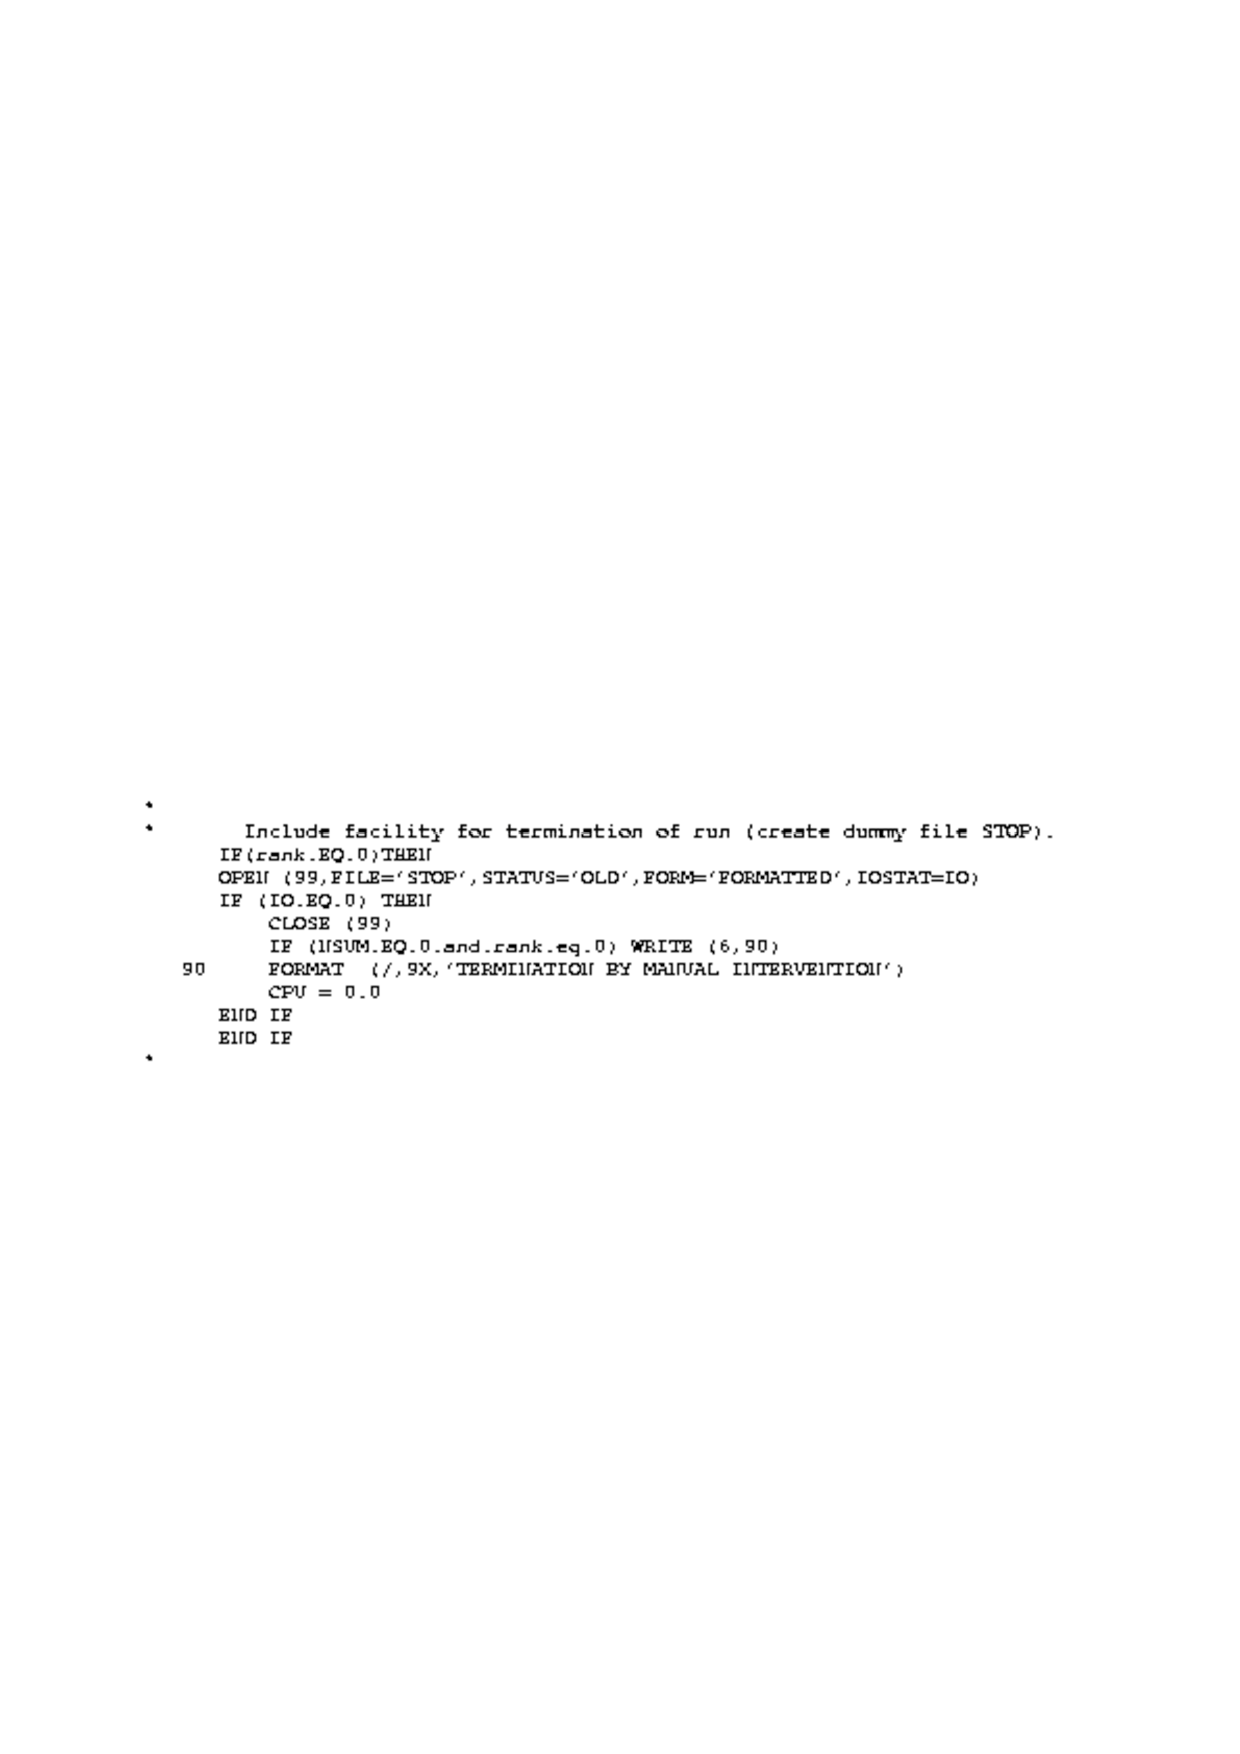
\epsfig{figure=fintgrF_p13.pdf,width=\textwidth}
  }
  \caption{Soft interruption of a simulation run in {\tt intgr.F}:
           If the dummy file ``STOP'' exists, then the run terminates.}
  \label{fig:integrF}
\end{figure}
%
The program writes out the current variables, saves a complete common
dump in {\tt comm.2\_*} and terminates.
The run can be restarted and continued from the same point where it
was left.

Before a restart, it is recommendable to copy or rename the files,
otherwise they may be overwritten.
Any file {\tt comm.2\_*} is restart-able.
The different names are just for getting common dumps at different
time units.
For example, if an irregular termination takes place, {\tt comm.2}
contains the data at some earlier time point, while {\tt comm.1}
always contains the last time data.

To restart a run, a different very short input control data file
needs to be used, because most of the control data are already
stored in {\tt comm.2\_*}~. \ff{The user should rename the desired {\tt comm.2\_*} file into {\tt comm.1}}
Only the first line corresponds to the standard input file,
but the first input variable, {\tt KSTART}, has to be changed
to ``2'' or higher.
In this case, the routine {\tt modify.F} will be entered.
%
\begin{center}
\begin{tabular}{|cp{10cm}|} \hline
{\bf KSTART} &  {\bf Function} \\  \hline
1      &  new run, start from initial values given in {\tt data.F}\\ \hline
2      &  continuation of a run without changes. With new NAMELIST input file style you can change any parameter, except for the position and velocity of the cluster in the galaxy RG(1:3) and VG(1:3), which should be calculated continuously. \\ \hline

\end{tabular}
\end{center}
%

The details of input and restart are discussed in Ch.~\ref{ch:inputvar}.


 

\section{Input variables} \label{ch:inputvar}

\textcolor{red}{
{\it The old input file has now been transformed to fortran NAMELIST format, which allows key=value pair reading like for an .ini file; the next subsection describes the new NAMELIST input format; while most input data stay the same (only the form of the input data file changes), some new data are appearing, which can now be changed directly using input. Previously these data had been compiled into the code. Also note that now initial and restart runs have the {\bf same} input files.}}

The input control file of NBODY6++ (see below), contains
order 90 parameters which guide one simulation run for
its technical and physical properties
(it is very similar but not identical to the one used for NBODY6).
As for the technical aspect, the file supervises the run e.g.
for its duration, intervals of the output, or error check;
the physical parameters concern the size of a cluster,
initial conditions, or a number of optional features 
related to the numerical problem to be studied.
The handling of this input file appears rather entangled
at first sight, for it has grown rather historically and
``ready--for--use'' than custom--oriented.
Thus, the input variables are read by different routines
(functions) in the code, and the nature of the parameters
are woven with each other in some cases.
Also, some parameters require additional input, such that the
total number of lines and parameters may vary.

In the following, we explain the main input file and give an
example of typical values for a simulation of an isolated
globular cluster.
Then, we proceed to the thresholds.\\

\noindent

{\tt\scriptsize
\begin{longtable}{|p{0.6in}|*{10}{l}|} 
\caption{\texttt{Input with all options}}
\label{table:allinput}\\
\hline
nbody6.F & \textcolor{red}{Input}& \textcolor{red}{Namelist}&  \textcolor{red}{INNBODY6} &&&&&&&\\
         & KSTART   & TCOMP    & TCRTP0   & isernb   & iserreg  
         & iserks   &          &          &          &          \\\hline
input.F &  \textcolor{red}{Input}& \textcolor{red}{Namelist}&  \textcolor{red}{ININPUT} &&&&&&&\\
        & N        & NFIX     &  NCRIT   & NRAND    & NNBOPT   &
           NRUN    & NCOMM    &          &          &          \\

        & ETAI     & ETAR     & RS0      & DTADJ    & DELTAT   &
           TCRIT    & QE       & RBAR     & ZMBAR    &          \\

        & KZ(1)    & KZ(2)    & KZ(3)    & KZ(4)    & KZ(5)    &
           KZ(6)    & KZ(7)    & KZ(8)    & KZ(9)~~~~KZ(10)&   \\
         
        & KZ(11)   & KZ(12)   & KZ(13)   & KZ(14)   & KZ(15)   &
           KZ(16)   & KZ(17)   & KZ(18)   & KZ(19)~~~KZ(20)&   \\
         
        & KZ(21)   & KZ(22)   & KZ(23)   & KZ(24)   & KZ(25)   &
           KZ(26)   & KZ(27)   & KZ(28)   & KZ(29)~~~KZ(30)&   \\
         
        & KZ(31)   & KZ(32)   & KZ(33)   & KZ(34)   & KZ(35)   &
           KZ(36)   & KZ(37)   & KZ(38)   & KZ(39)~~~KZ(40)&   \\
         
        & KZ(41)   & KZ(42)    & KZ(43)    & KZ(44)    & KZ(45)    &
          KZ(46)    & KZ(47)    & KZ(48)    & KZ(49)~~~KZ(50)&   \\
         
        & DTMIN    & RMIN     & ETAU     & ECLOSE   & GMIN     &
           GMAX     & SMAX     &          &          &          \\\hline

data.F & \textcolor{red}{Input}& \textcolor{red}{Namelist}&  \textcolor{red}{INDATA} &&&&&&&\\
       & ALPHA    & BODY1    & BODYN    & NBIN0    & NHI0     &
          ZMET     & EPOCH0   & DTPLOT   &          &          \\\hline
setup.F & \textcolor{red}{Input}& \textcolor{red}{Namelist}&  \textcolor{red}{INSETUP} &&&&&&&\\
         & AP0      & ECC      & N2       & SCALE   &       
         &          &          &          &(KZ(5)$=$2)&\\
         & AP0      & ECC      & SCALE    &         & 
         &          &          &          &(KZ(5)$=$3)&\\
         & AP0      & ECC      & SCALE    &         & 
&          &          &          &(KZ(5)$=$3)&\\
         & SEMI     & ECC      & M1       & M2      &
         &          &          &          &    (KZ(5)$=$4)&\\
         & ZMH      & RCUT     &          &         &
          \multicolumn{5}{r}{(KZ(5)$=$6\&\&KZ(24)<0)}&\\\hline

scale.F & \textcolor{red}{Input}& \textcolor{red}{Namelist}&  \textcolor{red}{INSCALE} &&&&&&&\\
         & Q        & VXROT    & VZROT    & RTIDE   &          
         &          &          &          &         &          \\ \hline

xtrnl0.F & \textcolor{red}{Input}& \textcolor{red}{Namelist}&  \textcolor{red}{INXTRNL0} &&&&&&&\\
         & GMG      & RG0      &          &         &
         &          &          &          &       (KZ(14)$=$2) & \\
         & GMG      & DISK~~~A &
         \multicolumn{6}{l}{B~~~VCIRC~~~RCIRC~~~GMB~~~
          AR~~~GAM~~~RG[1:3]~~~VG[1:3]} &       (KZ(14)$=$3) & \\
         & MP       & AP       & MPDOT    & TDELAY  &
         &           \multicolumn{4}{r}{(KZ(14)$=$3||KZ(14)$=$4)} & \\ \hline

binpop.F & \textcolor{red}{Input}& \textcolor{red}{Namelist}&  \textcolor{red}{INBINPOP} &&&&&&&\\
         & SEMI     & ECC      & RATIO    & RANGE   & NSKIP
         & IDORM    & \multicolumn{3}{r}{(KZ(8)$=$1||KZ(8)$>$4)} & \\ \hline

hipop.F & \textcolor{red}{Input}& \textcolor{red}{Namelist}&  \textcolor{red}{INHIPOP} &&&&&&&\\
         & SEMI     & ECC      & RATIO    & RANGE   & 
         &          &\multicolumn{3}{r}{(KZ(8)$>$0$\&\&$KZ(18)$>$1)}&\\ \hline
imbhinit.F & \textcolor{red}{Currently} & \textcolor{red}{not} & \textcolor{red}{supported} & \textcolor{red}{by} & \textcolor{red}{NAMELIST} & \textcolor{red}{Input} &&&&\\
         & MMBH  & XBH(1)   & XBH(2)    & XBH(3)  & VBH(1)
         & VBH(2)   & VBH(3)   & DTBH     &    (KZ(24)$=$1) & \\\hline

cloud0.F & \textcolor{red}{Currently} & \textcolor{red}{not} & \textcolor{red}{supported} & \textcolor{red}{by} & \textcolor{red}{NAMELIST} & \textcolor{red}{Input} &&&& \\
cloud0.F & NCL      & RB2      & VCL      & SIGMA   & CLM 
         & RCL2     &          &          &    (KZ(13)$>$0) & \\\hline
\end{longtable}
}


\vspace{0.2cm}
\noindent
\begin{longtable}{@{}p{1.5cm}p{13.0cm}}
\caption{\texttt{Input of \&INNBODY6, nbody6.F}}
\label{table:innbody6}\\\hline
%
KSTART  & Run control index\\
        & =1: new run (construct new model or read from \texttt{dat.10}) \\
        & =2: restart/continuation of a run, needs \texttt{comm.1}\footnote{the user should create a comm.1 file by copy-pasting the comm.2\_X, where X is the wanted NBU time value to restart the run. Notice that the same applies to KSTART $>$ 2; notice also that \\
        \texttt{cp -p `ls -rt comm.2* | tail -1` comm.1} \\
        is a nice unix way to automatically copy the last comm.2 to comm.1 }\\
%
TCOMP   & Maximum wall-clock time in seconds (parallel runs: wall clock)\\
%
TCRTP0  & Termination time in Myr \\
%
isernb  & For MPI parallel runs: only irregular block sizes larger than
          this value are executed in parallel mode
          (dummy variable for single CPU) \\
iserreg & For MPI parallel runs: only regular block sizes larger than
          this value are executed in parallel mode
          (dummy variable for single CPU) \\
iserks  & For MPI parallel runs: only ks block sizes larger than this value
           are executed in parallel mode 
          (dummy variable for single CPU) \\

\end{longtable}

\hrule
\noindent
\begin{longtable}{@{}p{1.5cm}p{13.0cm}}
\caption{\texttt{Input of \&ININPUT, input.F line 1}}
\label{table:ininput1}\\\hline
%
N       & Total number of particles (single + c.m.s.~of binaries;
          singles + 3$\times$c.m.s.~of binaries < NMAX$-$2)\\
NFIX    & Multiplicator for output interval of data on \texttt{conf.3} and
          of data for binary stars (output each DELTAT$\times$NFIX time steps; compare KZ(3) and KZ(6))\\
NCRIT   & Minimum particle number (alternative termination criterion) \\
NRAND   & Random number seed; any positive integer \\
%          (< LMAX$-$5) set in \texttt{params.h}\\
NNBOPT  & Desired optimal neighbour number (< LMAX$-$5)\\ %(R.Sp.)
NRUN    & Run identification index\\
NCOMM   & Multiplicator for frequency to store the dumping data (mydump); positive integer; basic frequency determined by DTADJ \\
\end{longtable}

\hrule
\noindent
\begin{longtable}{@{}p{1.5cm}p{13.0cm}}
\caption{\texttt{Input of \&ININPUT, input.F line 2}}
\label{table:ininput2}\\\hline
%
ETAI    & Time--step factor for irregular force polynomial\\
ETAR    & Time--step factor for regular force polynomial\\
RS0     & Initial guess for all radii of neighbour spheres ($N$--body units)\\
DTADJ   & Time interval for parameter adjustment and energy check ($N$--body units). In a good practice, DTADJ should be the same as, or larger than, DELTAT. \\
%%          (in TCR if KZ(35)=0, otherwise in $N$-body units)\\
DELTAT  & Time interval for writing output data and diagnostics,
          multiplied by NFIX ($N$--body units).\\
%%        & -- in units of $t_{\rm cr}$ if KZ(35) = 0;\\
%%$        & -- in scaled units if KZ(35) > 0.\\
%%        & for DTADJ=DELTAT (recommended) output data is written every
%%          adjust time\\
TCRIT   & Termination time ($N$--body units) \\
%*->             The _earlier_ termination criterion becomes active
QE      & Energy tolerance:\\
        & -- immediate termination if DE/E > 5*QE \& KZ(2) $\leq$ 1;\\
        & -- restart if DE/E > 5*QE \& KZ(2) > 1 and
         termination after second restart attempt.\\
RBAR    & Scaling unit in pc for distance ($N$--body units)\\
ZMBAR   & Scaling unit for average particle mass in solar masses\\
        & (in scale-free simulations RBAR and ZMBAR can be set to zero; depends on KZ(20)) \\
\end{longtable}

\hrule
\noindent
\begin{longtable}{@{}p{1.5cm}p{13.0cm}}
\caption{\texttt{Input of \&ININPUT, input.F lines 3-7}}
\label{table:ininput37}\\\hline
%
KZ(1)   & Save COMMON to file \texttt{comm.1}\\
        & $=1$: at end of run or when dummy file STOP is created\\
        & $=2$: every 100*NMAX steps\\
KZ(2)   & Save COMMON to file \texttt{comm.2}\\
        & $=1$: save at output time\\
        & $=2$: save at output time and restart simulation if energy error DE/E > 5*QE\\
KZ(3)   & Save basic data to file \texttt{conf.3} at output time (unformatted)\\
KZ(4)   & (Suppressed) Binary diagnostics on \texttt{bdat.4} (\# = threshold levels <10)\\
KZ(5)   & Initial conditions of the particle distribution, needs KZ(22)=0\\
        & $=0$: uniform \& isotropic sphere\\
        & $=1$: Plummer random generation\\
        & $=2$: two Plummer models in orbit (extra input)\\
        & $=3$: massive perturber and planetesimal disk (each pariticle 
              has circular orbit, constant separation along 
              radial direction between each neighbor and random phase)
              (extra input)\\
        & $=4$: massive initial binary (extra input)\\
        & $=5$: Jaffe model (extra input) \\
        & $\ge 6$: Zhao BH cusp model (extra input if KZ(24)<0) \\
KZ(6)   & Output of significant and regularized binaries at main output (\texttt{bodies.f})\\
        & $=1$: output regularized and significant binaries (|E|>0.1 ECLOSE)\\
        & $=2$: output regularized binaries only\\
        & $=3$: output significant binaries at output time and regularized binaries with time interval DELTAT\\
        & $=4$: output of regularized binaries only at output time\\
KZ(7)   & Determine Lagrangian radii and average mass, particle counters, average velocity, velocity dispersion, rotational velocity within Lagrangian radii (\texttt{lagr.f})\\
        & $=1$: Get actual value of half mass radius RSCALE by using current total mass\\
        & $\ge 2$: Output data at main output and \texttt{lagr.7} \\
        & $\ge 6$: Output Lagrangian radii for two mass groups at \texttt{lagr.31} and \texttt{lagr.32} (\texttt{lagr2.f}; based on KZ(5)=1,2; cost is O($N^2$))\\
        & ---- methods:\\
        & $=2,4$: Lagrangian radii calculated by initial total mass \\
        & $=3,\ge 5$: Lagrangian radii calculated by current total mass (The single/K.S-binary Lagrangian radii are still calculated by initial single/binary total mass)\\
        & $=2,3$: All parameters are averaged within the shell between two Lagrangian radii neighbors \\
        & $\ge 4$: All parameters are averaged from center to each Lagrangian radius\\
KZ(8)   & Primordial binaries initialization and output (\texttt{binpop.f})\\
        & ---- Initialization:\\
        & $=0$: No primordial binaries \\
        & $=1,\ge 3$: generate primordial binaries based on KZ(41) and KZ(42) (\texttt{binpop.F}) \\
        & $=2$: Input primordial binaries from first 2$\times$NBIN0 lines of \texttt{dat.10} \\
        & ---- Output:\\
        & $>0$: Save information of primordial binary that change member in \texttt{pbin.18}; binary diagnostics at main output (\texttt{binout.f}) \\
        & $\ge 2$: Output KS binary in \texttt{bdat.9}, soft binary in \texttt{bwdat.19} at output time\\
KZ(9)   & Binary diagnostics \\
        & $=1,3$: Output diagnostics for the hardest binary below ECLOSE in \texttt{hbin.39} (\texttt{adjust.f}) \\
        & $\ge 2$: Output binary evolution stages in \texttt{binev.17} (\texttt{binev.f}) \\
        & $\ge 3$: Output binary with degenerate stars in \texttt{degen.4} (\texttt{degen.f}) \\
KZ(10)  & K.S. regularization diagnostics at main output \\
        & $>0$: Output new K.S. information \\
        & $>1$: Output end K.S. information \\
        & $\ge 3$: Output each integrating step information\\
KZ(11)  & (Suppressed) \\
% KZ(11)  & Hierarchical systems (\texttt{hiarch.f})\\
%        & $=1,3$: write to \texttt{hia.12} \\
%        & $=2$: create primordial triples (\texttt{hipop.f})\\
%        & $=3$: both \\
KZ(12)  & $>0$: HR diagnostics of evolving stars with output time interval DTPLOT in \texttt{sse.83} (single star) and \texttt{bse.82} (K.S. binary) \\
        & $=-1$: used if KZ(19)$=0$ (see details in KZ(19) description)\\
KZ(13)  & Interstellar clouds \\
        & $=1$: constant velocity for new cloud\\
        & $>2$: Gaussian velocity for new cloud\\
KZ(14)  & External tidal force \\
        & $=0$: no external tidal field\\
        & $=1$: standard solar neighbor tidal field\\
        & $=2$: point-mass galaxy with circular orbit (extra input) \\
        & $=3$: point-mass + disk + halo + Plummer (extra input) \\
        & $=4$: Plummer model (extra input) \\
        & $=5$: Milky-Way potential (extra input) based on Galpy package (Bovy, 2015) \\
        & Note: Namelist input has all fields for values 2,3,4, but user must take care to put proper values \\
KZ(15)  & Triple, quad, chain and merger search. Note that \textit{triple} and \textit{quad} in KZ(15) means unperturbed triple and quad systems. \\
        & $\ge 1$: Switch on triple, quad, chain (KZ(30)>0) and merger search (\texttt{impact.f}) \\
        & $\ge 2$: Diagnostics at main output at begin and end of triple, quad \\
        & $\ge 3$: Save first five outer orbits every half period of wide quadruple before merger and stable quadruples accepted for merger in \texttt{quastab.89} \\
KZ(16)  & Auto-adjustment of regularization parameters. WARNING: not tested for large $N$ ($N>10^5$) systems with large mass range. \\
        & $\ge 1$: Adjust RMIN, DTMIN \& ECLOSE every DTADJ time \\
        & $\ge 3$: modify RMIN for GPERT > $0.05$ or < $0.002$ in chain; output diagnostics at \texttt{kscrit.77} \\
KZ(17)  & Auto-adjustment of ETAI, ETAR and ETAU by tolerance QE every DTADJ time (\texttt{check.f}). WARNING: not tested for large $N$ ($N>10^5$) systems with large mass range. \\
        & $\ge 1$: Adjust ETAI, ETAR \\
        & $\ge 2$: Adjust ETAU \\
KZ(18)  & Hierarchical systems \\
        & $=1,3$: diagnostics (\texttt{hiarch.f})\\
        & $\ge 2$: Initialize primordial stable triples, number is NHI0 (\texttt{hipop.F}) \\
        & $\ge 4$: Data bank of \textit{hierarchical} stable triple, quad in \texttt{hidat.87} (\texttt{hidat.f}) \\
KZ(19)  & Stellar evolution and mass loss scheme \\
        & $=0$: if KZ(12)$=-1$, the output data will keep the input data unit if KZ(22)$=2-4$ or $N$-body units if KZ(22)$=6-10$\\
        & $=1,2$: supernova scheme \\
        & $\ge 3$: Eggleton, Tout \& Hurley \\
        & $\ge 5$: extra diagnostics ({mdot.F}) \\
        & $=2,4$: input stellar parameters from \texttt{datsev.21}; 
                  read by (\texttt{instar.f}): \\
                & N lines of (MI, KW, M0, EPOCH1, OSPIN, MC); N is the number of particles in \texttt{datsev.21} and \texttt{dat.10} and has to be set accordingly in Nbody input file. \\
                & ~~~~~~   MI: current mass (solar mass) \\
                & ~~~~~~   KW: stellar type \\
                & ~~~~~~   M0: initial mass (solar mass) \\
                & ~~~~~~   EPOCH1: evolved age of star (AGE $= -$ EPOCH1 [Myr]) \\
                & ~~~~~~   OSPIN: angular velocity of star (may be zero if not relevant) \\
                & ~~~~~~   MC: core mass (solar mass, may be zero if not relevant) \\
        & $=4$: Take input data from other code (e.g. Monte Carlo); \\ 
        & first line of \texttt{datsev.21} in this case read by \texttt{start.F} to establish desired scaling: \\
                & 1 line of (TMOC,NZERO,RBAR,ZMBAR,TSTAR) \\ 
                &  \ff{(these data override data read or computed by Nbody before)} \\
                & ~~~~~~   TMOC: Cluster age in Myr \\
                & ~~~~~~   NZERO: Particle number at zero cluster age \\
                & ~~~~~~   RBAR, ZMBAR: scaling for radii and average \\  & ~~~~~~   TSTAR: 1Myr in model units; \\
KZ(20)  & Initial mass functions, need KZ(22)$=$0 or 9: \\
        & $=0$: self-defined power-law mass function using ALPHAS (\texttt{data.F}) \\
        & $=1$: Miller-Scalo-(1979) IMF (\texttt{imf.f}) \\
        & $=2,4$: KTG (1993) IMF (\texttt{imf2.f}) \\
        & $=3,5$: Eggleton-IMF (\texttt{imf2.f}) \\
        & $=6,7$: Kroupa(2001) (\texttt{imf2.f}), extended to Brown Dwarf regime (\texttt{imfbd.f}) \\
        & ---- Primordial binary mass \\
        & $=2,6$: random pairing (\texttt{imf2.f}) \\
        & $=3,4,5,7$: binary mass ratio corrected by $(m_1/m_2)\prime = (m_1/m_2)^{0.4}$ + constant (Eggleton, \texttt{imf2.f}) \\
        & $=8$: binary mass ratio $q=m_1/m_2$ ($m_2 \le m_1$) use distribtution $0.6 q^{-0.4}$ (Kouwenhoven) \\
%        & $=7$: Distinct mass bins  (\texttt{imf3.f}) \\
%        & $=8$: Scalo (1986)-IMF  with new random function RAN2 (\texttt{imf3.f}) \\
KZ(21)  & Extra diagnostics information at main output every DELTAT interval (\texttt{output.F}) \\
        & $\ge 1$: output NRUN, MODEL, TCOMP, TRC, DMIN, AMIN, RMAX, RSMIN, NEFF \\
        & $\ge 2$: Number of escapers NESC at main output will be counted by Jacobi escape criterion (cost is O($N^2$), \texttt{jacobi.f}) \\
KZ(22)  & Initialization of basic particle data mass, position and velocity (\texttt{data.F}) \\
        & ---- Initialization with internal method \\
        & $=0,1$: Initial position, velocity based on KZ(5), initial mass based on KZ(20) \\
        & $=1$: write initial conditions in \texttt{dat.10} (\texttt{scale.F}) \\
        & ---- Initialization by reading data from \texttt{dat.10} \\
        & $=2$: input through NBODY-format (7 parameters each line: mass, position(1:3), velocity(1:3))\\
        & $=3$: input through Tree-format (\texttt{data.F}) \\
        & $=4$: input through Starlab-format \\
        & $=6$: input through NBODY-format and do scaling\\
        & $=7$: input through Tree-Format and do scaling\\
        & $=8$: input through Starlab-format and do Scaling\\
        & $=9$: input through NBODY-format but ignore mass (first column) and use IMF based on KZ(20), then do scaling \\
        & $=10$: input through NBODY-format and all units are astrophysical units (mass: $M_\odot$; position: pc; velocity: km/s)\\
KZ(23)  & Removal of escapers (\texttt{escape.F})\\
        & $= 0, \ge 5$: no removal of escapers \\ 
        & $\ge 1$: remove escapers, and ghost particles generated by stellar evolution or two star coalescence (collision) \\
        & $=2,3,4$: write escaper diagnostics in \texttt{esc.11} and \texttt{escbin.31} for binary systems. \\
        & $=3$: tidal cutoff escape criterion (this option has been misused for tidal tail for a while) \\
        & $=4$: escape angles in main output \\
        & $\ge 5$: initialization \& integration of tidal tail (was wrongly: $\ge 3$)\\
%        & $=4$: write \#3 to diagnostics \\
KZ(24)  & =1: should not be used anymore, not supported (was: subsystems and IMBH)\\
        & =2: start with only black holes at T=0. \\
%KZ(25)  & Partial reflection of KS binary orbit (GAMMA < GMIN; suppressed) \\
KZ(25)  & Velocity kicks for white dwarfs (\texttt{kick.F}) \\
        & $=1$: Type 10 Helium white dwarf \& 11 Carbon-Oxygen white dwarf \\
        & $=2$: All WDs (type 10, 11 and type 12 Oxygen-Neon white dwarf) \\
KZ(26)  & Slow-down of two-body motion, increase the regularization integration efficiency \\
        & $\ge 1$: Apply to KS binary \\
        & $\ge 2$: Apply to chain \\
        & $=3$: Rectify to get better energy conservation \\
KZ(27)  & Two-body tidal circularization (Mardling \& Aarseth, 2001; Portegies Zwart et al. 1997) (for values 1,2) plus orbit shrinking of relativistic compact binaries (Rizzuto et al. 2021, 2022; Arca Sedda et al. 2021 (for values 3,4).
        (Please suppress in KS parallel version) \\
        & $=1$: sequential  \\
        & $=2$: chaos \\
        & $=3$: GR energy loss with sequential tides\\
        & $=4$: GR energy loss with chaos tides \\
        & $=-1$: Only detect collision and suppress coalescence \\
KZ(28)  & Magnetic braking. Gravitational radiation for NS or BH binaries is diabled here, since it is treated with KZ(27) now. \\
        & $\ge 1$: magnetic braking for NS \& BH (\texttt{brake.f}, \texttt{brake3.f})\\
        & $\ge 2$: Diagnostics at main output (\texttt{brake.f}) \\
        & $=3$: Input of ZMH = 1/SQRT(2*N) (Need KZ(5)$\ge$6) (\texttt{setup.F}) \\
        & $=4$: Set every star as type 13 Neutron star (Need KZ(27)=3) (\texttt{instar.f})  \\
KZ(29)  & (Reserved for new pulsar treatment decisions, not yet used)  \\
KZ(30)  & Hierarchical system regularization \\
        & $=-1$: Use chain only \\
        & $=0$: No triple, quad and chain regularization, only merger \\
        & $=1$: Use triple, quad and chain (\texttt{impact.f}) \\
        & $\ge 2$: Diagnostics at begin/end of chain at main output \\
        & $\ge 3$: Diagnostics at each step of chain at main output \\
KZ(31)  & Centre of mass correction after energy check (\texttt{cmcorr.f}) \\
KZ(32)  & Adjustment (increase) of adjust interval DTADJ, output interval DELTAT and energy error criterion QE based on binding eneryg of cluster (\texttt{check.f}) \\
KZ(33)  & Block-step statistics at main output (diagnostics) \\
        & $\ge 1$: Output irregular block step; and K.S. binary step if KZ(8)>0 \\
        & $\ge 2$: Output regular block step \\
KZ(34)  & Roche-lobe overflow \\
        & $=1$: Roche \& Spin synchronisation on binary with circular orbit (\texttt{synch.f}) \\
        & $=2$: Roche \& Tidal synchronisation on binary with circular orbit by BSE method (\texttt{bsetid.f}) \\
KZ(35)  & TIME reset to zero every 100 time units, total time is TTOT = TIME + TOFF (\texttt{offset.f})\\
KZ(36)  & (Suppressed) Step reduction for hierarchical systems \\
KZ(37)  & Neighbour list additions (\texttt{checkl.F}) \\
        & $\ge 1$: Add high-velocity particles into neighbor list \\
        & $\ge 2$: Add small time step particle (like close encounter particles near neighbor radius) into neighbor list \\
KZ(38)  & Force polynomial corrections during regular block step calculation \\
        & $=0$: no corrections \\
        & $=1$: all gains \& losses included \\
        & $=2$: small regular force change skipped \\
        & $=3$: fast neighbour loss only \\
KZ(39)  & Neighbor radius adjustment method \\
        & $=0$: The system has unique density centre and smooth density profile\\
        & $=1,\ge 3$: The system has no unique density centre or smooth density profile\\
        & ~~~~~~skip velocity modification of RS(I) (\texttt{regint.f}, \texttt{regcor\_gpu.f}) \\
        & ~~~~~~do not reduce neighbor radius if particle is outside half mass radius \\
        & ~~~~~~reduce RS(I) by multiply $0.9$ instead of estimation of RS(I) based on NNBOPT/NNB when neighbor list overflow happens (\texttt{fpoly0.F}, \texttt{util\_gpu.F}) \\
        & $=2,3$: Consider sqrt(particle mass / average mass) as the factor to determine the particle's neighbor membership. (\texttt{fpoly0.F}, \texttt{util\_gpu.F}) ({\bf Important to use if GPU is used for regular forces and neighbour lists!}) \\
KZ(40)  & $=0$: For the initialization of particle time steps, use only force and its first derivative to estimate. This is very efficent.\\
        & $>0$: Use fpoly2 (second and third order force derivatives calculation) to estimate the initial time steps. This method provides more accurate {\bf initial (only)} time steps and avoid incorrent time steps for some special cases like initially cold systems, but the computing cost (initial model only) is much higher ($O(N^2)$)\\
KZ(41)  & proto-star evolution of eccentricity and period for primordial binaries initialization (\texttt{proto\_star\_evol}, \texttt{binpop.F}) \\
KZ(42)  & Initial binary distribution \\
        & $=0$: RANGE>0: uniform distribution in log(semi) between SEMI0 and SEMI0/RANGE \\
        & ~~~~~~~ RANGE<0: uniform distribution in semi between SEMI0 and -1*RANGE. \\
        & $=1$: linearly increasing distribution function $f=0.03438*logP$ \\
        & $=2$: $f=3.5logP/[100+(logP)**2]$ \\
        & $=3$: $f=2.3(logP-1)/[45+(logP-1)**2]$; This is a ``3rd'' iteration when  pre-ms evolution is taken into account with KZ(41)=1 \\
        & $=4$: $f=2.5(logP-1)/[45+(logP-1)**2]$; This is a ``34th'' iteration when pre-ms evolution is taken into account with KZ(41)=1 and RBAR<$1.5$ \\
        & $=5$: Duquennoy \& Mayor 1991, Gaussian distribution with mean $\log{P}=4.8$, SDEV in $\log{P}=2.3$. Use Num.Recipes routine \texttt{gasdev.f} to obtain random deviates given ``idum1'' \\
%        & $=6$: eigen-evolution (Pavel Kroupa \& Rosemary Mardling)\\
KZ(43)  & Reserved for LPS+ code \url{https://github.com/kaiwu-astro/lps_plus} \\
KZ(44)  & (Unused) \\
KZ(45)  & $>0$: Computation of Moments of Inertia (with Chr. Theis) in output listing (\texttt{ellan.f}) \\
KZ(46)  &  HDF5/BINARY/ANSI format output and global parameter output (main output, see chapter~\ref{ch:output} for details) \\
        &  $=1,3$: HDF5(if HDF5 is compiled)/BINARY format\\
        &  $=2,4$: ANSI format \\
        &  $=1,2$: Only output active stars with time interval defined by KZ(47) \\
        &  $=3,4$: Output full particle list with time interval defined by KZ(47) \\
KZ(47)  &  Frequency for KZ(46) output. Should be non-negative integer. \\
        &  Output data with time interval $0.5^{KZ(47)} \times SMAX$ \\
KZ(48)  & $=0,1$: if 1 reduced HDF5 output (no 2nd and 3rd derivatives of force); warning: if KZ(40)=0 initial values wrong, undefined. \\
KZ(49)  & (Unused) \\
KZ(50)  & For event data bank, similar to MOCCA. Uses file units with numbers above 200; still under development; to switch on set to 1. \\

\end{longtable}

\hrule
\noindent
\begin{longtable}{@{}p{1.5cm}p{13.0cm}}
\caption{\texttt{Input of \&ININPUT, input.F line 8-9}}
\label{table:ininput89}\\\hline
%
DTMIN   & Time--step criterion for regularization search \\
RMIN    & Distance criterion for regularization search \\
ETAU    & Regularized time-step parameter (6.28/ETAU steps/orbit) \\
ECLOSE  & Binding energy per unit mass for hard binary (positive) \\
GMIN    & Relative two-body perturbation for unperturbed motion \\
GMAX    & Secondary termination parameter for soft KS binaries \\
SMAX    & Maximum time-step (factor of 2 commensurate with 1.0) \\
LEVEL   & \textcolor{red}{Stellar Evolution Level (see Kamlah et al. 2022), new input element} \\
\multicolumn{2}{l}{\textcolor{red}{\&INSSE, \&INBSE, \&INCOLL: new NAMELIST blocks read after LEVEL by subroutine READSE,}} \\
\multicolumn{2}{l}{\textcolor{red}{called from input.F; if blocks are empty in input, defaults according to LEVEL taken.}}
\end{longtable}

% & \texttt{if (kz(4).gt.0)} (suppressed now) \\
%DELTAS  & Output interval for binary search (in TCR; suppressed) \\
%ORBITS  & Minimum periods for binary output (level 1) \\
%GPRINT  & Perturbation thresholds for binary output (9 levels) \\

\hrule
\noindent
\begin{longtable}{@{}p{1.5cm}p{13.0cm}}
\caption{\texttt{Input of \&INDATA, data.F}}
\label{table:indata}\\\hline
%
ALPHAS  & Power-law index for initial mass function, routine \texttt{data.F}\\
BODY1   & Maximum particle mass before scaling (based on KZ(20); solar mass unit)\\
BODYN   & Minimum particle mass before scaling\\
NBIN0   & Number of primordial binaries (need KZ(8)>0) \\
        & -- by routine \texttt{imf2.F} using a binary IMF (KZ(20)$\ge$2)\\
        & -- by routine \texttt{binpop.F} splitting single stars (KZ(8)>0)\\
        & -- by reading subsystems from \texttt{dat.10} (KZ(22)$\ge$2)\\
NHI0    & Number of primordial hierarchical systems (need KZ(18)$\ge$2)\\
ZMET    & Metal abundance (in range 0.03 - 0.0001) \\
EPOCH0  & Formation time of stellar population, should be $\le$ 0, since at time of simulation start the stellar AGE is -EPOCH0 (in $10^6$ yrs); note that datsev.21 allows to input individual stellar ages \\
DTPLOT  & Plotting interval for stellar evolution HRDIAG (N-body units; $\ge$ DELTAT) \\
\end{longtable}

\hrule
\noindent
\begin{longtable}{@{}p{1.5cm}p{13.0cm}}
\caption{\texttt{Input of \&INSETUP, setup.F, KZ(5)>1}}
\label{table:insetup}\\\hline
       & \texttt{if (kz(5)=2)} \\\hline
APO    & Separation of two Plummer models in $N$--body units (SEMI = APO/(1 $+$ ECC). (Notice SEMI will be limited between $2.0$ and $50.0$) \\
ECC    & Eccentricity of two-body orbit (ECC $\ge$0 and ECC < $0.999$) \\
N2     & Membership of second Plummer model (N2 <= N) \\
SCALE  & Scale factor for the second Plummer model, second cluster will be generated by first Plummer model with $X \times SCALE$ and $V \times \sqrt{SCALE}$($\ge 0.2$ for limiting minimum size) \\\hline
       & \texttt{if (kz(5)=3)} \\\hline
APO    & Separation between the perturber and Sun in $N$--body units \\
ECC    & Eccentricity of orbit (=1 for parabolic encounter) \\
SCALE  & Perturber mass scale factor, perturber mass = Center star mass $\times$ SCALE (=1 for Msun) \\\hline
       & \texttt{if (kz(5)=4)} \\\hline
SEMI   & Semi-major axis (slightly modified; ignore if ECC > 1) \\
ECC    & Eccentricity (ECC > 1: NAME = 1 \& 2 free-floating) \\
M1     & Mass of first member (in units of mean mass) \\
M2     & Mass of second member (rescaled total mass = 1) \\\hline
       & \texttt{if (kz(5)$\ge$6) and (kz(24)<0)} \\\hline
ZMH    & Mass of single BH (in N-body units) \\
RCUT   & Radial cutoff in Zhao cusp distribution (MNRAS, 278, 488) \\
\end{longtable}

\hrule
\noindent
\begin{longtable}{@{}p{1.5cm}p{13.0cm}}
\caption{\texttt{Input of \&INSCALE, scale.F}}
\label{table:inscale}\\\hline
\texttt{scale.F:} & \\\hline
%
Q       & Virial ratio (routine \texttt{scale.F}; Q=0.5 for equilibrium) \\
VXROT   & XY--velocity scaling factor (> 0 for solid-body rotation) \\
VZROT   & Z--velocity scaling factor (not used if VXROT = 0) \\
RTIDE   & Unscaled tidal radius for KZ(14)=2 and KZ(22)$\ge$2. If not zero, RBAR = RT/RTIDE where RT[pc] is tidal radius calculated from input GMG and RG0\\
\end{longtable}

\hrule
\noindent
\begin{longtable}{@{}p{1.5cm}p{13.0cm}}
\caption{\texttt{Input of \&XTRNL0, xtrnl0.F}}
\label{table:indata}\\\hline
       & \texttt{if (kz(14)=2)} \\\hline
GMG    & Point-mass galaxy (solar masses, linearized tidel field in circular orbit) \\
RG0    & Central distance (in kpc) \\\hline
       & \texttt{if (kz(14)=3)} \\\hline
GMG    & Point-mass galaxy (solar masses) \\
DISK   & Mass of Miyamoto disk (solar masses) \\
A      & Softening length in Miyamoto potential (in kpc) \\
B      & Vertical softening length (kpc) \\
VCIRC  & Galactic circular velocity (km/sec) at RCIRC (=0: no halo) \\
RCIRC  & Central distance for VCIRC with logarithmic potential (kpc) \\
GMB    & Dehnen model budge mass (solar masses)\\
AR     & Dehnen model budge scaling radius (kpc)\\
GAM    & Dehnen model budge profile power index gamma \\  
RG(1:3) & Initial cluster position vector (kpc); DISK+VCIRC=0, VG(3)=0: A(1+E)=RG(1), E=RG(2) . Note that upon restart, RG is not read from input; saved value is used instead.\\
VG(1:3) & Initial cluster velocity vector (km/s). Note that upon restart, VG is not read from input; saved value is used instead. \\\hline
       & \texttt{if (kz(14)=3,4)} \\\hline
MP     & Total mass of Plummer sphere (in scaled units) \\
AP     & Plummer scale factor (N-body units; square saved in AP2) \\
MPDOT  & Decay time for gas expulsion (MP = MP0/(1 + MPDOT*(T-TD)) \\
TDELAY & Delay time for starting gas expulsion (T > TDELAY) \\\hline
       & \texttt{if (kz(14)=5)} \\\hline
RG(1:3) & Initial cluster position vector (kpc) . Note that upon restart, RG is not read from input; saved value is used instead.\\
VG(1:3) & Initial cluster velocity vector (km/s). Note that upon restart, VG is not read from input; saved value is used instead. \\ 
\end{longtable}

\hrule
\noindent
\begin{longtable}{@{}p{1.5cm}p{13.0cm}}
\caption{\texttt{Input of \&INBINPOP, binpop.F, \\\phantom{xxxxxxxx}if (kz(8)=1 or kz(8)>2)}}
\label{table:inbinpop}\\\hline
%
SEMI0   & Initial semi-major axis limit\\
ECC0    & Initial eccentricity \\
        & $<0$: thermal distribution, $f(e)=2e$ \\
        & $\ge 0$ and $\le 1$: fixed value of eccentricity\\
        & $=20$: uniform distribution \\
        & $=30$: distribution with $f(e)=0.1765/(e^2)$ \\
        & $=40$: general $f(e)=a*e^b$, $e0<=e<=1$ with $a=(1+b)/(1-e0^{(1+b)})$, current values: $e0=0$ and $b=1$ (thermal distribution) \\
RATIO   & KZ(42)$\le 1$: Binary mass ratio $M1/(M1 + M2)$\\
        & KZ(42)$=1.0$: $M1 = M2 = \langle M \rangle$\\
RANGE   & KZ(42)$=0$: semi-major axis range for uniform logarithmic distribution; \\
        & not used for other KZ(42)\\
NSKIP   & Binary frequency of mass spectrum (starting from body \#1)\\
IDORM   & Indicator for dormant binaries ($>0$: merged components)\\
\end{longtable}

\hrule
\noindent
\begin{longtable}{@{}p{1.5cm}p{13.0cm}}
\caption{\texttt{Input of \&INHIPOP, hipop.F\\\phantom{xxxxxxx} if (kz(8)>0 and kz(18)>1)}}
\label{table:inhipop}\\\hline
%
SEMI  &  Max semi-major axis in model units (all equal if RANGE = 0) \\
ECC   &  Initial eccentricity ($<0$ for thermal distribution) \\
RATIO &  Mass ratio ($= 1.0$: $M1 = M2$; random in [$0.5\thicksim0.9$]) \\
RANGE &  Range in SEMI for uniform logarithmic distribution ($> 0$) \\
\end{longtable}

\hrule
\noindent


%\hrule
%\noindent
%\begin{longtable}{@{}p{1.5cm}p{13.0cm}}
%\texttt{intide.F:}& \texttt{if (kz(27)>0)} (currently suppressed)
%RSTAR &  Size of typical star in A.U. \\
%IMS   &  # idealized main-sequence stars \\
%IEV   &  # idealized evolved stars \\
%RMS   &  Scale factor for main-sequence radii (>0: fudge factor) \\
%REV   &  Scale factor for evolved radii (initial size RSTAR)\\
%\end{longtable}

\hrule
\noindent
\begin{longtable}{@{}p{1.5cm}p{13.0cm}}
\texttt{cloud0.F:}& \texttt{if (kz(13)>0)} 
\textcolor{red}{Input currently NOT working with Namelist input method}
\\\hline
%
NCL   &  Number of interstellar clouds \\
RB2   &  Radius of cloud boundary in pc (square is saved) \\
VCL   &  Mean cloud velocity in km/sec \\
SIGMA &  Velocity dispersion (KZ(13)>1: Gaussian) \\
CLM   &  Individual cloud masses in solar masses (maximum MCL) \\
RCL2  &  Half-mass radii of clouds in pc (square is saved) \\
\end{longtable}

\vspace{1cm}

\section*{Stellar Evolution}

Stellar evolution is invoked by KZ(19)=1,2 or KZ(19)$\ge$3, offering two different
schemes.
The simpler one is KZ(19)=1, while the more complex one, K(19)$\ge$3,
is based on the Cambridge stellar evolution package
(Hurley, Pols, Tout 2000). The common envelope, roche transfering binaries are also considered. 
The main effects are changing stellar masses, radii, and luminosities,
which give rise to cluster mass loss.
The mass is assumed to escape from the cluster immediately and
possible collisions depend on stellar radii.

With the additional option KZ(12)>0, information on binaries and
single stars is written on two files (for binaries, unit 82, file \texttt{bev.82}; for single stars,
unit 83, file \texttt{sev.83}) in regular time intervals determined by
TPLOT (See details in Section~Output).
{\bf need to check for possibly more important information from Kamlah paper we missed out.}


\section*{Fortran NAMELIST based input}

The new input file is printed below. All input is grouped into a NAMELIST input block; our input is grouped according to the subroutines which read the lines ({\tt nbody6, input, data, setup, scale, xtrnl0, binpop, hipop}). In addition to that single and stellar evolution parameters, and stellar collision parameters, are read from the NAMELIST input blocks {\tt sse, bse, coll}. For every such NAMELIST input block the values can be given in the form {\tt name=value}, where {\tt name} is the variable name in the code. An input block in the file has to begin with {\tt \&NML} and terminate with {\tt /}, where {\tt NML} is the name of the block used in the code and in the input data file (e.g. {\tt INNBODY6}. Line breaks can be put in at liberty.

The principle of Fortran NAMELIST input is that the sequence in which the data are given is not relevant; if a variable of an input block is not given, it is possible to define it in the code (give default values). This principle is currently used for the input blocks {\tt sse, bse, coll} - a new variable {\tt LEVEL} of type {\tt CHARACTER*1} for the stellar evolution level is read at the end of the {\tt input} block - it can be Level A,B,C, or 0. Stellar Evolution Levels A,B,C are defined in Kamlah et al. (2022). If {\bf no data are given in} {\tt sse,bse,coll} {\bf the default values defined in Table A1 of that paper are used} (for Levels A,B,C, respectively). Level {\tt 0} (``zero'') corresponds to a run without stellar evolution. Note that {\tt LEVEL='0'} has to be provided in the input file for the case of no stellar evolution.

All variables can be redefined individually, for the first run and for any restart alike. For example
{\tt \&INSSE nsflag=3 /} in the input file will redefine nsflag different from the default. {\bf Notice: for all input blocks other than} {\tt sse, bse, coll} {\bf there are currently NO default values defined, so the user has to be responsible to provide a value for every required input} (as it was before). Values for all data in {\tt sse, bse, coll} are now always printed in the main output listing.


\begin{center}
\textcolor{red}{New Input File Example using Fortran NAMELIST}
\label{table:inputfile}\\
\fbox{\parbox{12.0cm}
{\tt
\&INNBODY6 \\
KSTART=1,TCOMP=1.0E8,TCRTP0=1000.0,\\isernb=40,iserreg=40,iserreg=0 / \\
\\
\&ININPUT \\
N=105000,NFIX=1,NCRIT=10,NRAND=43532,NNBOPT=80,NRUN=1,NCOMM=1, \\
ETAI=0.01,ETAR=0.01,RS0=0.15,DTADJ=1.0,DELTAT=1.0,\\TCRIT=1000.0,QE=1.0,RBAR=1.223,ZMBAR=0.7, \\
KZ(1:10)= 1 1 1 0 1 0 3 2 3 2 \\
KZ(11:20)=0 1 0 2 2 0 0 0 3 6 \\
KZ(21:30)=1 2 2 0 2 2 3 2 0 2 \\
KZ(31:40)=1 0 2 2 1 0 1 1 2 1 \\
KZ(41:50)=0 0 0 0 0 1 3 0 1 0 , \\
DTMIN=2.5E-6,RMIN=8.E-5,ETAU=0.1,ECLOSE=1.0,\\GMIN=1.0E-06,GMAX=0.01,SMAX=1.0, \\
Level='C' / \\
\\
\&INSSE / \\
\\
\&INBSE / \\
\\
\&INCOLL / \\
\\
\&INDATA \\
ALPHAS=2.35,BODY1=150.0,BODYN=0.08,NBIN0=5000,NHI0=0,\\ZMET=0.001,EPOCH0=0,DTPLOT=1.0 / \\
\\
\&INSETUP SEMI=,ECC=,APO=,N2=,SCALE=,ZM1=,ZM2,ZMH,RCUT= / \\
\\
\&INSCALE \\
Q=0.5,VXROT=0.0,VZROT=0.0,RTIDE=0.0 / \\
\\
\&INXTRNL0 \\
GMG=7.54E10,RG0=5.19,DISK=,A=,B=,VCIRC=,RCIRC=,GMB=,\\AR=,GAM=,RG=,,,VG=,,,MP=,AP2=,MPDOT=,TDELAY= / \\
\\
\&INHIPOP /
}
}
\end{center}


Note that empty placeholders like {\tt DISK=,} can be ignored, they just signal for the interested user where to put values if special options are chosen (as given in Table~\ref{table:allinput} and following tables).
\newpage

In the following all variables of the input blocks {\tt sse, bse, coll} are given, which are not displayed in the box above:

\begin{center}
\fbox{\parbox{12.0cm}
{\tt
\&INSSE \\
ecflag,wdflag,nsflag,psflag,mdflag,bhflag,kmech,mch,
mxns0,mxns1,nwind,bwind,flbv,disp,ecsig,wdsig1,wdsig2,wdkmax,\\
vvfac / \\
\&INBSE \\
lambd1,alphac,bhspinfl,kicktype,xk2,xk3,acc1,acc2,
xbeta,xxi,epsnov,eddfac,gamm1 / \\
\&INCOLL  \\
fctorcl /
}
}
\end{center}

A few notes: some variables had to be renamed compared to their genuine name in a certain subrouttine, in order to be unique throughout the code. These are:

\begin{center}
\fbox{\parbox{12.0cm}
{\tt
nwind = neta in mlwind.f \\
vvfac = vfac in kick.F \\
lambd1 = lambda in comennv.f \\
alphac = alpha1 in comenv.f \\
xk2 = k2 in hrdiag.f \\
xk3, xbeta, xxi = k3, beta, xi in mdot.F and roche.f 
}
}
\end{center}

The following variables are not explicitly documented in Kamlah et al. (2022), but included into the new namelist blocks: {\tt mch, mxns0, mxns}. These are the Chandrasekhar mass and two levels of neutron star masses; their defaults are defined equally for {\bf ALL} levels of stellar evolution as: {\tt mch=1.44, mxns0=1.8, mxns1 = 2.5} (solar masses).

Furthermore {\tt xk2, xk3, acc1} are not documented in the cited paper; their default values are set as {\tt xk2 = xk3 = 0.21, acc1 = 3.920659d8}; again these defaults do {\bf NOT} depend on stellar evolution and are taken from predefined values in the code before.
The value of {\tt k2 (xk2)} had been earlier hard-coded to be 0.21 in {\tt hrdiag.f}; now it can be set in input, the value from the input data is still used in {\tt hrdiag.f} to define {\tt k2}. {\tt hrdiag.f} argument list contains {\tt k2}, which is used in several other routines. 

The variables in the new input blocks {\tt sse, bse, coll} have been allocated now in three new Fortran {\tt common} blocks, with respective names. Due to that in several routines declarations of variables had to be adjusted, these are: \\[0.5cm]
\noindent
{\tt mlwind, mdot, comenv, corerd, roche, kick, kickGW, hrdiag, coal, mix}
 \\[0.5cm]
For handling the new input style using Fortran {\tt NAMELIST} input the following routines needed adjustment: \\[0.5cm]
\noindent
{\tt nbody6, input, modify, data, scale, xtrnl0, binpop, hipop}
\\[0.5cm]
The file {\tt input.F} contains a new subroutine {\tt READSE}, which handles read and write for all data in blocks {\tt sse, bse, coll}; both for initial run (called from {\tt input}) and for any restart (called from {\tt modify}.

\textcolor{red}{
Note that at the current time (April 2023) input done from the routinesIch 
{\tt cloud0, hotsys, ttinit, imbhinit }
{\bf fails! It is not working, and may be obsolete or updated in the future.}}


\section*{The old input file style (obsolete since April 2023)}

This input file was used until April 2023.
A typical input file can look like as follows.
It defines a new simulation running for 1,000,000 CPU--minutes
with $N=16,000$ particles distributed from a Plummer profile
(KZ(5)=1).
The run may alternatively terminate when TCRIT=1000.0 $N$--body units.
or if the final particle number of NCRIT=10 has been reached.
The output and adjustment time interval DELTAT/DTADJ are 1.0 N-body unit.
The initial mass function follows Kroupa, (2001) with mass ranging
from $m_{\rm max}=20.0 M_{\odot}$ to $m_{\rm min}=0.08 M_{\odot}$ (BODY1 and BODYN).
The initial virial ratio is 0.5 (equilibrium). The stellar 
evolution is switched on (KZ(19)=3) and initial metallicity is 0.001. 
Multiples and chain regularization are switched on (KZ(15)=2 and KZ(30)=2).
It uses solar neighbor tidal field (KZ(14)=1). 

\vspace{\baselineskip}
\noindent
\begin{center}
\fbox{\parbox{12.0cm}
{\tt
1 1000000.0 1.E6 40 40 640 \\
16000 1 10 43532 100 1 1 \\
0.02 0.02 0.1 1.0 1.0 1000.0 2.0E-05 1.0 0.7 \\
0 1 1 0 1 0 4 0 0 2 \\
0 1 0 1 2 1 0 0 3 6 \\
1 0 2 0 0 2 0 0 0 2 \\
1 0 2 1 1 0 1 1 0 0 \\
0 0 0 0 0 0 0 0 0 0 \\
1.0E-06 1E-4 0.2 1.0 1.0E-06 0.01 1.0 \\
2.35 20.0 0.08 0 0 0.001 0 1.0 \\
0.5 0.0 0.0 0.0 \\
7.54E10 5.19 \\
0.0005 -1.0 1.0 5.0 5 0 \\
\\
KSTART, TCOMP, TCRTP0, isernb,iserreg,iserks                  (nbody6.F)\\
N, NFIX, NCRIT, NRAND, NNBOPT, NRUN, NCOMM                    (input.F)
ETAI, ETAR, RS0, DTADJ, DELTAT, TCRIT, QE, RBAR, ZMBAR        (input.F)\\
(KZ(J),J=1,50)                                                (input.F)\\
DTMIN, RMIN, ETAU, ECLOSE, GMIN, GMAX, SMAX                   (input.F)\\
ALPHA, BODY1, BODYN, NBIN0, NHI0, ZMET, EPOCH0, DTPLOT        (data.F)\\
Q, VXROT, VZROT, RSPH2                                        (scale.F)\\
NBIN, SEMI0, ECC0, RATIO,RANGE, NSKIP, IDORM                  (binpop.f)\\
GMG, RG0                                                      (xtrnl0.F) KZ(14)=2 \\
GMG, DISK, A, B, VCIRC, RCIRC, GMB, AR, GAM,RG(1-3),VG(1-3)   (xtrnl0.F) KZ(14)=3 \\
SEMI0, ECC0, RATIO,RANGE, NSKIP, IDORM                        (binpop.f) KZ(8)=1,KZ(8)=3 \\
SEMI0, ECC0, RATIO,RANGE                                      (hipop.F) KZ(8)>0,KZ(18)>1
}
}
\end{center}


\section*{Input variables for primordial Binaries}

Many star clusters contain initial hard binaries with binding
energies much larger than the thermal energy
(the threshold ECLOSE is a suitable division between hard and
soft binaries).
There are two ways to initialise primordial binaries:

{\it The first} one always starts from some initial mass function (IMF)
provided by the routines \texttt{imf.f} or \texttt{imf2.f}.
The option KZ(8)=1 or $\ge 3$ invokes the routine \texttt{binpop.F}, which reads the
last line of the input file containing NBIN and the parameters of
their distribution (see above).
In this case, binaries are created either by random pairing of
single stars obtained from the IMF or by splitting them, depending on
the value of KZ(20) (see above).

{\it The second} way assumes that particle data, including the binaries,
are provided via the input data on file $\,$\texttt{dat.10}$\,$ (as e.g.
in the Kyoto--II collaborative experiment).
In such a case KZ(8)=2 and NBIN0 should be set to the expected number of primordial binaries
from the file. The code will first create NBIN0 centers of masses, and then use those
for scaling, before regularizing the pairs and the calculation begins.

A typical input file with primordial binaries looks as follows.
Here, we use binary random pairing from \texttt{imf2.f} and \texttt{binpop.F}
(KZ(20)=6 and KZ(8)=3, respectively) for 1000 initial binaries.
The semi-major axes of binaries use uniform distribution in log(semi) with a range from $41.3$ AU to $0.00413$ AU.
The eccentricity of binaries use thermal distribution. 
It was created from this input file running for 1000 time units.
Stellar evolution was also switched on in this file (KZ(19)=3).
In the package of the code, the file \texttt{N10k\_B1k.input} is
included.
%
%\vspace{\baselineskip}
%\noindent
\begin{center}
\fbox{\parbox{12.0cm}
{\tt
1 1000000.0 1.E6 40 40 640 \\
10000 1 10 43532 100 1 \\
0.02 0.02 0.17 1.0 1.0 800.0 5.0E-05 1.0 0.7 \\
0 1 1 0 1 0 4 3 0 2 \\
0 1 0 1 2 1 0 0 3 6 \\
1 0 2 0 0 2 0 0 0 2 \\
1 0 2 1 1 0 1 1 0 0 \\
0 0 0 0 0 0 0 0 0 0 \\
5.0E-06 3E-4 0.2 1.0 1.0E-06 0.01 0.5 \\
2.35 100.0 0.08 1000 0 0.001 0 1.0 \\
0.5 0.0 0.0 0.0 \\
2E-4 -1.0 1.0 1E4 5 0 
}
}
\end{center}



\vspace{0.7cm}

\section*{Restart}

\textcolor{red}{
Note that the new fortran NAMELIST based input does {\bf NOT} make any differences between input files for a restart or for a new run. The only difference will be the KSTART variable, which can bei either 1 or 2. All other values of KSTART will become obsolete; see next subsection.
}

It's very common that in the computer cluster every job has running time limit,
or the simulation stop due to some energy conservation problem or the normal stop
when the stop criterion is reached. In this case the user may want to continue the
simulation from the last time point. Thus the input parameter should changed to 
restart mode. The first line of input shown above combined together with two 
extra lines (See the description of KSTART in the parameter table above).
A simple example is :

\begin{center}
\fbox{\parbox{12.0cm}
{\tt
2 1000000.0 1.E6 40 40 640 
}
}
\end{center}

Here KSTART=2 means every parameter keeps the same value as before and just restarts from
the last saved file \texttt{comm.1}. If the user wants to change some parameters
of simulation, KSTART=3,5 can be set. For example:

\begin{center}
\fbox{\parbox{12.0cm}
{\tt
3 1000000.0 1.E6 40 40 640 \\
2.0 2.0 0.0 0.0 0.0 0.0 16 0 0.0 0.0
}
}
\end{center}

This restart file will change DTADJ and DELTAT to $2.0$. The KZ(16) is changed to 0.
All other parameters that are set to $0.0$ (TADJ, TNEXT, TCRIT, QE) keep same as before.

 

\section{Thresholds for the variables} \label{ch:thresholds}



Before the compilation of the code (Chapter~\ref{ch:startrun}),
the parameter file ({\tt params.h}) should be consulted to check
whether some vector dimensions are in the desired range.
Most important are
%
\begin{itemize}
\item the maximum particle number {\tt NMAX},
\item the maximum number of regularised KS pairs {\tt KMAX}, and
\item the maximum number of neighbours per particle {\tt LMAX}.
\end{itemize}


The particles are saved in various lists which serve to distinguish
between their funcionality.
The table below explains their nomenclature.
``KS--pairs'' are particles that approach each other in a hyperbolic
encounter; they are given a special treatment by the code (see
Chapter~\ref{ch:regularization}).
If NPAIRS is the amount of KS--pairs, then IFIRST = 2*NPAIRS + 1
is the first single particle (not member of a KS pair), and N the
last one.
NTOT = N + NPAIRS is the total number of particles plus c.m.'s.
Therefore NMAX, the dimension of all vectors containing particle
data should be at least of size N + KMAX, where N is the number of
particles and KMAX the maximum number of expected KS pairs.
If one starts with single particles, KMAX = 10 or 20 should usually
be enough, but in clusters with a large number of primordial binaries,
KMAX must be large.
%
\begin{longtable}{@{}p{1.5cm}p{13.0cm}}
N:      & Total number of particles\\
NBIN0:  & number of primordial binaries (physical bound stars)\\
NBIN:   &  ??? \\
NPAIRS: & Number of binaries (KS--pairs, see Chapter~\ref{ch:regularization}),
          transient unbound pairs as well as persistent binaries\\
NTOT:   & = N + NPAIRS; \\
        & Number of single particles plus centres of masses of
          regularized (KS) pairs \\
KMAX:   & threshold for the amount of allowed KS pairs\\
NMAX:   & = N + KMAX; threshold for the total number of particles and
          the centre of masses
\end{longtable}



\vspace{2cm}
\noindent
\fbox{Hier gibt's noch ein Bildchen!}



 

\begin{landscape}
%\setlength{\textwidth}{23.0cm}


\section{How to read the diagnostics}

The diagnostics is the ASCII readable text printed on unit 6
{\it stdout} (``out1000'' in Chapter~\ref{ch:startrun}) that
gives a brief overview of the global status and progress of
the cluster simulation.
Different routines write into that file, depending on the options
chosen as the input variables. The following lines occur:\\

\noindent
\hrule
\begin{minipage}{18cm}
{\tiny
\begin{verbatim}
               N  NFIX  NCRIT  NRAND  NNBOPT  NRUN

            1000     5     10   1006      50     1


             ETAI      ETAR      RS0       DTADJ     DELTAT     TCRITp    TCRIT     QE        RBAR       ZMBAR

             1.0E-02   2.0E-02   3.0E-01   1.0E+01   1.0E+01   1.0E+06   2.0E+01   2.0E-05   1.0E+00   7.0E-01


            OPTIONS

           1  2  3  4  5  6  7  8  9 10 11 12 13 14 15 16 17 18 19 20 21 22 23 24 25 26 27 28 29 30 31 32 33 34 35 36 37 38 39 40

           1  1  1  0  1  0  4  0  0  2  1  0  0  0  1  1  1  0  0  0  1  0  1  0  0  2  0  0  0  2  0  0  2  0  1  0  1  1  0  1


            OPTIONS BK:

           1  2  3  4  5  6  7  8  9 10

           0  0  0  0  0  0  0  0  0  0


            DTMIN     RMIN      ETAU      ECLOSE    GMIN      GMAX

            1.0E-04   1.0E-02   1.0E-01   1.0E+00   1.0E-06   1.0E-02

  ****** NOTE: new random number seed initialisation!
  ****** AND new ran2 from new ed. of Press et al.
\end{verbatim}
}
\end{minipage} \hfill
%
\begin{minipage}{4.5cm}
\begin{center}
written by the routine:
{\tt input.F}\\[2ex]
Usage: Repetition of the input variables
\end{center}
\end{minipage}

\vspace{2ex}
\noindent
\hrule


\vspace{1ex}
\noindent
\begin{minipage}{18cm}
{\tiny
\begin{verbatim}
            STANDARD IMF    ALPHA = 2.35  BODY1 = 20.0  BODYN = 0.10 ZMASS = 3.36752E+02 NBIN0=    0 ZMET = 0.00 EPOCH0 = 0.00

            ...............................................................................................................

            BINARY STAR IMF:   NB =  400  RANGE =  3.27E+01  2.14E-01 ZMB = 3.74E+02  <MB> = 9.36E-01

            SINGLE STAR IMF:   NS = 1200  RANGE =  7.76E+00  1.01E-01 ZMS = 5.25E+02  <MS> = 4.38E-01
\end{verbatim}
}
%{\it These lines if routine {\tt imf2.f} is used (KZ(20)$\ge$2):}
IMF power law index, max.~mass, min.~mass, total mass,
\# of primordial bin., metallicity,
evolution.~epoch [Myrs].\\
..................................................................\\
number of objects, mass range, average mass before scaling.
\end{minipage} \hfill
%
\begin{minipage}{4.5cm}
\begin{center}
{\tt data.F},\\
(if KZ(20)=0 \& BODY1$\ne$BODYN)\\[1ex]
or\\[1ex]
{\tt imf2.F}, if KZ(20)$\ge$2\\[2ex]
Information about initial mass function (IMF).
%(only if an IMF is chosen)
\end{center}
\end{minipage}

\vspace{2ex}
\noindent
\hrule


\vspace{1ex}
\noindent
\begin{minipage}[t]{18cm}
{\tiny
\begin{verbatim}
            SCALING:   SX =  1.00421D+00  E = -2.49E-01  M(1) = 5.94E-02  M(N) = 2.97E-04  <M> = 1.00E-03

            TIME SCALES:   TRH = 2.8E+01  TCR = 2.8E+00  2<R>/<V> = 2.8E+00


     PHYSICAL SCALING:    R* = 1.0000E+00  M* = 7.0000E+02  V* = 1.7348E+00  T* = 5.6466E-01  <M> = 7.0000E-01
                          SU = 4.4335E+07  AU = 2.0627E+05  YRS = 3.5408E+06
\end{verbatim}
}
scaling factor for energy, total energy,
max.~mass, min.~mass, average mass {\it after scaling};\\
Spitzer's half-mass relaxation time, crossing time obtained from
total energy and mass, crossing time obtained from virial radius
(see \ref{ch:nbtime});\\
information about physical scaling: values of one $N$--body unit
in length (pc), mass (solar masses), velocity (km/s), time (million years),
average mass of particles (solar massses), astronomical units (one
$N$--body unit) and years (one $N$--body unit).
\end{minipage} \hfill
%
\begin{minipage}{4.5cm}
\begin{center}
{\tt scale.F, units.f}
%(scaling of the cluster properties)
\end{center}
\end{minipage}

\vspace{2ex}
\noindent
\hrule


\vspace{1ex}
\noindent
\begin{minipage}{18cm}
{\tiny
\begin{verbatim}
fpoly1 time=  0.1200000035762785     
fpoly2 time=  0.2100000062584875     
\end{verbatim}
}
CPU (wall clock in parallel execution) time for initialising
the force and its time derivative ({\tt fpoly1, fpoly\_mpi.f}) 
and the second and third time derivative of the force
({\tt fpoly2, fpoly2\_mpi.f}).
The mpi-versions are called for initialisation in case of
parallel runs.
\end{minipage} \hfill
%
\begin{minipage}{4.5cm}
\begin{center}
{\tt start.F}
\end{center}
\end{minipage}

\vspace{2ex}
\noindent
\hrule


\vspace{1ex}
\noindent
\begin{minipage}[t]{18cm}
{\tiny
\begin{verbatim}
    TIME  M/MT:    1.00D-02  2.00D-02  5.00D-02  1.00D-01  2.00D-01  3.00D-01  4.00D-01  5.00D-01  7.00D-01  9.00D-01  1.00D+00 <RC
      0.0 RLAGR:   1.52D-01  1.81D-01  1.91D-01  2.83D-01  4.33D-01  5.22D-01  6.17D-01  7.52D-01  1.16D+00  1.96D+00  5.86D+00  2.97D-01
      0.0 AVMASS:  6.26D-04  4.26D-03  6.13D-04  9.45D-04  7.82D-04  1.11D-03  1.09D-03  8.35D-04  9.19D-04  1.25D-03  9.01D-04  1.23D-03
      0.0 NPARTC:        17         9         2        53       130        90        91       122       216       163       107        90
      0.0 SIGR2:   2.19D-01  1.70D-01  7.37D-01  2.44D-01  1.89D-01  2.33D-01  2.16D-01  2.43D-01  1.72D-01  8.36D-02  5.09D-02  2.09D-01
      0.0 SIGT2:   2.01D-01  8.25D-02  4.46D-02  2.12D-01  3.39D-01  2.42D-01  1.71D-01  1.83D-01  1.51D-01  1.03D-01  6.16D-02  1.63D-01
      0.0 VROT:   -8.34D-02  4.41D-01 -6.28D-01  3.14D-02 -1.54D-01 -9.44D-02 -6.45D-02  1.17D-02  5.35D-02  1.98D-02 -3.46D-02  4.46D-01
\end{verbatim}
}
Time, specification of the Lagrangian radii, core radius\\
Time, Lagrangian radii, core radius (if primordial binaries: separately
 for singles and binaries, not shown above)\\
Time, average mass between Lagrangian radii, ~ avmass in the core\\
Time, number of particles within the shell, ~ in the core\\
Time, radial velocity dispersion within the shell, ~ in the core\\
Time, tangential vel.~dispersion within the shell, ~ in the core\\
Time, rotational vel. within the shell, ~ in the core (not shown above)\\
\end{minipage} \hfill
%
\begin{minipage}{4.5cm}
\begin{center}
{\tt lagr.F}
%(Lagrangian data)
\end{center}
\end{minipage}

\vspace{2ex}
\noindent
\hrule


\vspace{1ex}
\noindent
\begin{minipage}[t]{18cm}
{\tiny
\begin{verbatim}
  0 ADJUST:  TIME =    1.00000D+01  T[Myr] =     5.65  Q = 0.52  DE =  -1.403819E-05  E =  -2.500038E-01 EBIN=   0.000000E+00 EMERGE=   0.000000E+00
\end{verbatim}
}
rank, ``ADJUST:'', total time in NB units, physical time,
virial ratio, relative energy error, total energy,
total energy of regularized pairs, energy of mergers
\end{minipage} \hfill
%
\begin{minipage}{4.5cm}
\begin{center}
{\tt adjust.F}
\end{center}
\end{minipage}

\vspace{1ex}
\noindent
\hrule


\vspace{1ex}
\noindent
\begin{minipage}[c]{18cm}
{\tiny
\begin{verbatim}
  RMIN = 1.1E-03  DTMIN = 3.5E-05 RHOM = 3.5E+02 RSCALE = 9.5E-01 RSMIN = 2.2E-01  ECLOSE = 1.05  TC =    3
  PE  N       ttot      treg      tirr      tpredtot  tint      tinit      tks      ttcomm    tadj     tmov      tprednb  tsub     tsub2    xtsub1   xtsub2
   0  1000     41.46000     29.54      7.23      0.63     40.39      0.99      0.07      0.00      0.59      0.00      1.50      0.00      0.00  0.00000D+00  0.00000D+00
\end{verbatim}
}
close encounter distance and minimum time step (for regularization search,
updated from input parameters if KZ(16)=1), maximum density, virial radius,
minimum neighbour sphere, hard binary threshold energy, 
total run time in units of initial crossing times\\
number of processors, number of particles, total processing time,
total regular processing, total irregular processing, processing of
prediction, time spent in {\tt intgrt.F}, for initialisation, for
KS integration, for communication, for adjust and energy check,
for overhead of moving data in parallel runs, for neighbour predictions,
for MPI communication after irregular (tsub) and regular (tsub2) blocks,
number of bytes transferred respectively. From xtsub1/tsub and xtsub2/tsub2
the sustained bandwidth of MPI communication can be read off.
Note, that the determination of these quantities involves a
certain overhead by many calls of {\tt cputim.F} per block,
so for critically large production runs one may want to comment
these out (most of them in {\tt intgrt.F}).
\end{minipage} \hfill
%
\begin{minipage}{4.5cm}
\begin{center}
{\tt adjust.F}
\end{center}
\end{minipage}

\vspace{1ex}
\noindent
\hrule

\vspace{1ex}
\noindent
\begin{minipage}[c]{18cm}
{\tiny
\begin{verbatim}
  0 T =   10.0  N = 1000  <NB> = 20  KS =    0  NM = 0 MM = 0 NS =  1000 NSTEPS =    1610624       273    321696       1016  DE =  -0.140382E-04  E =        -0.250004

 NRUN =  1  M# =  1  CPU = 6.91000E-01  TRC =  0.0  DMIN = 6.6E-05 6.6E-05 1.0E+02 1.0E+02  AMIN = 1.0E+02  RMAX = 0.0E+00  RSMIN = 0.22  NEFF =   128

    <R>  RTIDE  RDENS   RC      NC   MC   RHOD   RHOM  CMAX   <Cn>  Ir/R    UN    NP    RCM    VCM         AZ     EB/E   EM/E   TCR     T6
 #1 0.95   9.5   0.21  0.08      5  0.073  159.   350.    5.  37.0  0.13     0     0    0.000  0.0000   0.006197  0.000  0.000  2.83     5

       NNPRED    NBCORR  NBFULL  NBVOID  NRCONV    NICONV  NBSMIN  NBDIS  NBDIS2  NCMDER  NBDER  NFAST  NBFAST    NBLOCK     NBPRED
 #2     20204    294307       0      98    2664      9227    1576      0       0      33      0      0       0     58132    3045868

     NKSTRY  NKSREG  NKSHYP     NKSPER  NPRECT  NKSREF  NKSMOD  NTTRY  NTRIP  NQUAD  NCHAIN  NMERG  NSTEPT  NSTEPQ  NSTEPC    NBLCKR    NBFLUX
 #3   14463      45      33          0       0       0       0      0      0      0       0      0       0       0       0     10333   1903963
\end{verbatim}
}
time, actual particle number, average neighbour number, number of KS pairs,
number of merged KS pairs, number of hierarchical subsystems, number of single
stars, step numbers (irregular, irr. c.m., regular, KS), relative energy error
since last output, total energy\\
several more lines uncommented here....
\end{minipage} \hfill
%
\begin{minipage}{4.5cm}
\begin{center}
{\tt output.F}
\end{center}
\end{minipage}

\vspace{2ex}
\noindent
\hrule



\vspace{1ex}
\noindent
\begin{minipage}[t]{18cm}
{\tiny
\begin{verbatim}
 STEP I     0    3   63   91  154  220  160  133  109   44   19    4
 STEP R     0    4   77  133  249  310  179   45    3
 Max Speedup Irr:     4 3.76D+00    8 6.82D+00   16 1.14D+01   32 1.66D+01   64 2.15D+01  128 2.49D+01  256 2.66D+01  512 2.74D+01 1024 2.77D+01
 Max Speedup Reg:     4 3.71D+00    8 6.69D+00   16 1.12D+01   32 1.67D+01   64 2.22D+01  128 2.62D+01  256 2.91D+01  512 3.04D+01 1024 3.11D+01
\end{verbatim}
}
histogram of distribution of irregular (STEP I), regular (STEP R)\\
If there are p step distribution (not appearing here, STEP U,
in physical time), statistics of parallel work for irr. and reg.
steps, figures given are theoretical speedups for infinitely
fast communication (limit of large block sizes)
\end{minipage} \hfill
%
\begin{minipage}{4.5cm}
\begin{center}
{\tt levels.f}
\end{center}
\end{minipage}

\vspace{2ex}
\noindent
\hrule



\vspace{1ex}
\noindent
\begin{minipage}[c]{18cm}
{\tiny
\begin{verbatim}
         END RUN    TIME[Myr] =   11.29  TOFF/TIME/TTOT=      0.00000000     20.00000000     20.00000000  CPUTOT =    1.6  ERRTOT =-5.15000D-05  DETOT =-1.28197D-05


        0 INTEGRATION INTERVAL =   20.00    NIRR=    3237662 NIRRB=       1245 NREG=     779010 NKS=       4625


          PER TIME UNIT: NIRR= 1.61883D+05 NIRRB= 6.22500D+01 NREG= 3.89505D+04 NKS= 2.31250D+02
  Total CPU=   97.11000289410342     
\end{verbatim}
}
This is the regular end of a run giving:
the integration time, total cumulative absolute and relative errors,
cumulative number of regular, irregular, KS steps,
the step numbers per time unit and the total CPU
(wall clock for parallel) time in minutes.\\
\end{minipage} \hfill
%
\begin{minipage}{4.5cm}
\begin{center}
\vspace{1cm}
{\tt adjust.F}
\end{center}
\end{minipage}


\noindent
\hrule
\vfill
\end{landscape}

\newpage

To check a regular stop of the run, look at the end of the
diagnostics first.
If there are failures, the line ``{\tt CALCULATION HALTED}''
appears and means that the energy conservation could not be
guaranteed.
A restart with smaller steps (ETAI, ETAR) and larger neighbour
number NNBOPT may cure the problem, but not always;
persistent problems should be reported to Rainer Spurzem.

The unix command on the output file, e.g.\\

\noindent
{\tt
  {\it homedir}> grep ADJUST out1000
}\\

\noindent
produces an overview of the accuracy (energy error at every
DTADJ interval).
It may show where problems originated; a restart from the last
ADJUST before the error with smaller output intervals is one
way to look after it.
Watch out, because sometimes errors are not reproducible,
because changes in ADJUST intervals change frequencies of
prediction and small differences can build up.
A quick possibility to see the real evolution of the system
is to {\tt grep} for the lines with Lagrangian radii and other
quantities (see above), which can directly be plotted, e.g.\
with gnuplot, because the first column is always the time.



 
%%% Prallel runs.

\section{Runs on parallel machines} \label{ch:parallel}



For parallel runs, the file {\tt mpif.h} is very important,
and system specialists should be consulted in addition to us
what to use.
Again, for some standard systems templates are provided
(e.g.\ {\tt mpif.t3e.h } $\:$ or $\:$ {\tt mpif.mpich.h}).
The routine providing CPU--time measurements, {\tt cputim.F}~,
and the use of the function {\tt flush.f} may need special
attention depending on the hardware.


 
%%% Chapter 7 of Emil's PhD-thesis.

\section{The Hermite integration method} \label{ch:hermite}


Each particle is completely specified by its mass $m$,
position $\mathbf r_0$, and velocity $\mathbf v_0$,
where the sub\-script $0$ denotes an initial value at a
time $t_0$.
The equation of motion for a particle $i$ is given by
its momentary acceleration $\mathbf a_{0,i}$ due to
all other particles and its time derivative
$\dot{\mathbf a}_{0,i}$ as
%
\begin{eqnarray}
\mathbf a_{0,i} &=& -\sum_{i \neq j} G m_j\frac{\mathbf R}{R^3} ,
                 \label{eq:accel0}\\
%
\dot{\mathbf a}_{0,i} &=& -\sum_{i \neq j} G m_j
          \left [ \frac{\mathbf V}{R^3}
                  + \frac{3\mathbf R(\mathbf V \cdot \mathbf R)}{R^5}
          \right ] , \label{eq:accel1}
\end{eqnarray}
%
where $G$ is the gravitational constant;
$\mathbf R = \mathbf r_{0,i} - \mathbf r_{0,j}$ is
the relative coordinate;
$R = |\mathbf r_{0,i} - \mathbf r_{0,j}|$ the modulus;
and $\mathbf V = \mathbf v_{0,i} - \mathbf v_{0,j}$
the relative space velocity to the particle $j$.

The Hermite scheme employed in NBODY6++ follows the trajectory
of the particle by firstly ``predicting'' a new position
and new velocity for the next time step $t$.
A Taylor series for $\mathbf r_i(t)$ and $\mathbf v_i(t)$
is formed:
%
\begin{eqnarray}
\mathbf r_{p,i}(t) &=& \mathbf r_0
                + \mathbf v_0(t-t_0)
                + \mathbf a_{0,i}\frac{(t-t_0)^2}{2}
                + \dot{\mathbf a}_{0,i}\frac{(t-t_0)^3}{6} ,
         \label{eq:predr} \\
%
\mathbf v_{p,i}(t) &=&  \mathbf v_0
                + \mathbf a_{0,i}(t-t_0)
                + \dot{\mathbf a}_{0,i}\frac{(t-t_0)^2}{2} .
          \label{eq:predv}
\end{eqnarray}
%
The predicted values of $\mathbf r_p$ and $\mathbf v_p$,
which result from this simple Taylor series evaluation,
using the force and its time derivative at $t_0$,
do not fulfil the requirements for an accurate
high--order integrator;
they just give a first approximation to $\mathbf r_1$
and $\mathbf v_1$ at the upcoming time $t_1$.
Even if the time step, $t_1 - t_0$, is chosen
impracticably small, a considerable error will
quickly occur, let alone the inadequate
computational effort.
Therefore, an improvement is made by the Hermite
interpolation which approximates the higher
accelerating terms by another Taylor series:
%
\begin{eqnarray}
\mathbf a_i(t) &=& \mathbf a_{0,i}
                   + \dot{\mathbf a}_{0,i} \cdot (t - t_0)
                   + \frac{1}{2}\mathbf a_{0,i}^{(2)} \cdot (t-t_0)^2
                   + \frac{1}{6}\mathbf a_{0,i}^{(3)} \cdot (t-t_0)^3 ,
          \label{eq:accp0} \\
%
\dot{\mathbf a}_i(t) &=& \dot{\mathbf a}_{0,i}
                   + \mathbf a_{0,i}^{(2)} \cdot (t-t_0)
                   + \frac{1}{2}\mathbf a_{0,i}^{(3)} \cdot (t-t_0)^2 .
          \label{eq:accp1}
\end{eqnarray}
%
Here, the values of $\mathbf a_{0,i}$ and $\dot{\mathbf a}_{0,i}$
are already known, but a further derivation of equation
(\ref{eq:accel1}) for the two missing orders on the right
hand side turns out to be quite cumbersome.
Instead, one determines the additional acceleration terms
from the predicted (``provisional'') $\mathbf r_p$ and
$\mathbf v_p$;
we calculate their acceleration and time derivative
according to the equations (\ref{eq:accel0}) and
(\ref{eq:accel1}) anew and call these new terms
$\mathbf a_{p,i}$ and $\dot{\mathbf a}_{p,i}$,
respectively.
Because these values ought to be generated by the former
high--order terms also (which we avoided),
we put them into the left--hand sides of (\ref{eq:accp0})
and (\ref{eq:accp1}).
Solving equation (\ref{eq:accp1}) for $\mathbf a_{0,i}^{(2)}$,
then substituting it into (\ref{eq:accp0}) and simplifying yields
the third derivative:
%
\begin{eqnarray}
\mathbf a_{0,i}^{(3)}
        &=& 12\frac{\mathbf a_{0,i} - \mathbf a_{p,i}}%
                   {(t - t_0)^3}
           + 6\frac{\dot{\mathbf a}_{0,i} + \dot{\mathbf a}_{p,i}}%
                   {(t - t_0)^2} . \label{eq:accel3}
\end{eqnarray}
%
Similarly, substituting (\ref{eq:accel3}) into
(\ref{eq:accp0}) gives the second derivative:
%
\begin{eqnarray}
\mathbf a_{0,i}^{(2)}
        &=&  -6\frac{\mathbf a_{0,i} - \mathbf a_{p,i}}%
                    {(t - t_0)^2}
             -2\frac{2\dot{\mathbf a}_{0,i} + \dot{\mathbf a}_{p,i}}%
                    {t - t_0}.  \label{eq:accel2}
\end{eqnarray}
%
Note, that the desired high--order accelerations are found
just from the combination of the low--order terms for
$\mathbf r_0$ and $\mathbf r_p$.
We never derived higher than the first derivative, but
achieved the higher orders easily through (\ref{eq:accel0})
and (\ref{eq:accel1}).
This is called the Hermite scheme.


Previously, a four--step Adams--Bashforth--Moulton integrator
was used (especially in NBODY5, \cite{a_85}),
however, the new Hermite scheme allows twice as large timesteps
for the same accuracy.
Also its storage requirements are less
\cite{m_91b}, \cite{ma_92}, \cite{a_99a}, \cite{a_99b}.

Finally, we extend the Taylor series for $\mathbf r_i(t)$
and $\mathbf v_i(t)$, eqs.~(\ref{eq:predr}) and
(\ref{eq:predv}), by two more orders,
and find the ``corrected'' position $\mathbf r_{1,i}$
and velocity $\mathbf v_{1,i}$ of the particle $i$
at the computation time $t_1$ as
%
\begin{eqnarray}
\mathbf r_{1,i}(t)
        &=&  \mathbf r_{p,i}(t)
           + \mathbf a_{0,i}^{(2)}\frac{(t - t_0)^4}{24}
           + \mathbf a_{0,i}^{(3)}\frac{(t - t_0)^5}{120} , \\
%
\mathbf v_{1,i}(t)
        &=&  \mathbf v_{p,i}(t)
           + \mathbf a_{0,i}^{(2)}\frac{(t - t_0)^3}{6}
           + \mathbf a_{0,i}^{(3)}\frac{(t - t_0)^4}{24} .
\end{eqnarray}
%
The integration cycle for other upcoming steps may now be
repeated from the beginning, eqs.\ (\ref{eq:accel0}) and
(\ref{eq:accel1}).
The local error in $\mathbf r$ and $\mathbf v$ within the two time
steps $\Delta t = t_1 - t_0$ is expected to be of order
${\cal O}(\Delta t^5)$, the global error for a fixed physical
integration time scales with ${\cal O}(\Delta t^4)$ \cite{m_91a}.


 

\section{Individual and block time steps}
\label{ch:timesteps}

Stellar systems are characterized by a huge dynamical range in
radial and temporal scales.
The time scale varies e.g.\ in a star cluster from orbital periods
of binaries of some days up to the relaxation of a few hundred
million years, or even billions of years.
Even if we put for a moment the very close binaries aside,
which are treated differently (by regularization methods),
there typically is a large dynamic range in the average local
stellar density from its centre to the very outskirts, where it
dissolves into the galactic tidal field.
In a classical picture, the two closest bodies would determine
the time--step of force calculation for the whole rest of the
system.
However, for bodies in regions where the changes of the force are
relatively small, a permanent re--computing of the terms appears
time consuming.
So, in order to economize the calculation, these objects shall
be allowed to move a longer distance before a recomputation
becomes necessary.
In between there is always the possibility to acquire particle
positions and velocities via a Taylor series prediction,
as described in Chapter~\ref{ch:hermite}.
This is the idea of a vital method for assigning different
time--steps, $\Delta t = t_1 - t_0$, between the force
computations, the so--called ``individual time--step scheme''
\cite{a_63}, which was later advanced to the hierarchical
block steps.


%%%%%%%%%%%%   Figure for block time step scheme   %%%%%%%%%%%%
\begin{figure}[ht]
%
\centering
\framebox{
\unitlength1cm
\begin{picture}(10,6.2)
   % lower horizontal line (time step)
   \thinlines
      \put(0.5,1){\line(1,0){9.0}}                 % time axis
      \multiput(0.5,1.125)(0.5,0){18}{\line(0,-1){0.25}} % tickmarks
      \put(0.43,0.5){0}                             % ticknames
      \put(0.93,0.5){1}
      \put(1.43,0.5){2}
      \put(2.43,0.5){4}
      \put(4.43,0.5){8}
      \put(5.8,0.5){time steps}
      \put(8.3,0.5){16}
   % time steps of particles
   \thicklines
      \multiput(0.5,2.2)(0.5,0){12}{\vector(1,0){0.5}}
          \multiput(6.5,2.2)(1.0,0){2}{\vector(1,0){1.0}}
      \multiput(0.5,3.2)(1.0,0){4}{\vector(1,0){1.0}}
          \multiput(4.5,3.2)(2.0,0){2}{\vector(1,0){2.0}}
      \multiput(0.5,4.2)(2.0,0){2}{\vector(1,0){2.0}}
          \multiput(4.5,4.2)(1.0,0){2}{\vector(1,0){1.0}}
          \multiput(6.5,4.2)(0.5,0){4}{\vector(1,0){0.5}}
      \multiput(0.5,5.2)(4.0,0){2}{\vector(1,0){4.0}}
   % vertical dotted lines
      \put(0.5,1.8){\line(0,1){3.8}}
      \dottedline{0.2}(1.0,1)(1.0,2.1)
      \dottedline{0.2}(1.5,1)(1.5,3.1)
      \dottedline{0.2}(2.0,1)(2.0,2.1)
      \dottedline{0.2}(2.5,1)(2.5,4.1)
      \dottedline{0.2}(3.0,1)(3.0,2.1)
      \dottedline{0.2}(3.5,1)(3.5,3.1)
      \dottedline{0.2}(4.0,1)(4.0,2.1)
      \dottedline{0.2}(4.5,1)(4.5,5.1)
      \dottedline{0.2}(5.0,1)(5.0,2.1)
      \dottedline{0.2}(5.5,1)(5.5,2.1)
          \dottedline{0.2}(5.5,3.7)(5.5,4.6)
          \dottedline{0.2}(7.0,3.7)(7.0,4.6)
          \dottedline{0.2}(7.5,3.7)(7.5,4.6)
          \dottedline{0.2}(8.0,3.7)(8.0,4.6)
      \dottedline{0.2}(6.0,1)(6.0,2.1)
      \dottedline{0.2}(6.5,1)(6.5,4.1)
%      \dottedline{0.2}(7.0,1)(7.0,2.1)
      \dottedline{0.2}(7.5,1)(7.5,2.1)
%      \dottedline{0.2}(8.0,1)(8.0,2.1)
      \dottedline{0.2}(8.5,1)(8.5,5.1)
   % vertical ticknames
      \put(0.0,2.1){$i$}
      \put(0.0,3.1){$k$}
      \put(0.0,4.1){$l$}
      \put(0.0,5.1){$m$}
      \put(0.0,5.8){particles}
%      \put(0.0,5.7){blocks}
\end{picture}
}%
  \vspace{1ex}
  \caption{Block time steps exemplary for four
           particles.}
  \label{pic:its}
\end{figure}


Each particle is assigned its own $\Delta t_i$ which is
first illustrated for the case of ``block time--steps''
in Figure \ref{pic:its}.
The particle named $i$ has the smallest time step at the
beginning, so its phase space coordinates are determined at
each time step.
The time step of $k$ is twice as large as $i$'s,
and its coordinates are just extrapolated (``predicted'')
at the odd time steps, while a full force calculation is
due at the dotted times.
The step width may be altered or not after the end of the
integration cycle for the special particle, as demonstrated
for $k$ and $l$ beyond the label ``8''.
The time steps have to stay commensurable with both,
each other as well as the total time, such that a
hierarchy is guaranteed.
This is the block step scheme.

As a first estimate, the rate of change of the acceleration
seems to be a reasonable quantity for the choice of the time
step:
$\Delta t_i \propto \sqrt{ \mathbf a_i / \dot{\mathbf a}_i }$.
But it turns out that for special situations in a many-body
system, it provides some undesired numerical errors.
After some experimentation, the following formula was adopted
\cite{a_85}:
%
\begin{eqnarray}
\Delta t_i = \sqrt{
           \eta \frac{|\mathbf a_{1,i}||\mathbf a_{1,i}^{(2)}| +
                      |\dot{\mathbf a}_{1,i}|^2 }
                     {|\dot{\mathbf a}_{1,i}||\mathbf a_{1,i}^{(3)}| +
                      |\mathbf a_{1,i}^{(2)}|^2 }
                  } ,    \label{eq:timestep}
\end{eqnarray}
%
where $\eta$ is a dimensionless accuracy parameter which
controls the error.
In most applications it is taken to be $\eta \approx$ 0.01
to 0.02, see also next chapter.

For the block--time steps, the synchronization is made
by taking the next--lowest integer of $\Delta t_i$;
the time steps are quantized to powers of 2 \cite{m_91a}.
Then, there will be a group (block) of several particles
which are due to movement at each time step.
If one keeps the exact $\Delta t_i$'s evaluated from
(\ref{eq:timestep}) for each particle, the commensurability
is destroyed, and we arrive at the so--called ``individual
time steps'';
in this case, there exists one sole particle being due.
The latter concept is realized in the earlier codes
NBODY1, NBODY3, NBODY5, where a neighbour scheme is renounced.
NBODY4, NBODY6, and NBODY6++ use a block step scheme.

% In the running code, the time--steps are adjusted to their
% appropriate values fairly quick. % Makino & Aarseth (1992)
% Although successive steps normally change smoothly,
% it is prudent to restrict the growth by a stability factor
% of 1.2. % Aarseth (1985)

Subsystems like star binaries, triples or a similar subgroups
(they are termed KS pairs, chains, hierarchies) enter the
time--step scheme with their respective centre's of masses only.
Their internal motion is treated in a different way by a
regularized integration (Chapter~\ref{ch:regularization}).



 

\section{The Ahmad--Cohen scheme}


The computation of the full force for each particle
in the system makes simulations very time--consuming
for large memberships.
Therefore, it is desirable to construct a method in
order to speed up the calculations while retaining
the collisional approach.
One way to achieve this is to employ a ``neighbour scheme'',
suggested by \cite{ac_73}.


The basic idea is to split the force polynomial (\ref{eq:accp0})
on a given particle $i$ into two parts, an irregular and a
regular component:
%
\begin{eqnarray}
\mathbf a_i = \mathbf a_{i,{\rm irr}} + \mathbf a_{i,{\rm reg}} .
\end{eqnarray}
%
The irregular acceleration $\mathbf a_{i,{\rm irr}}$ results
from particles in a certain neighbourhood of $i$
(in the code, FI and FIDOT are the irregular force and its
time derivative at the last irregular step;
internally some routines use FIRR and FD as a local variable).
They give rise to a stronger fluctuating gravitational force,
so it is determined more frequently than the regular one
of the more distant particles that do not change their
relative distance to $i$ so quickly
(in the code, FR and FRDOT are the regular force and its time
derivative at the last regular step; some routines use
as a local variable FREG and FDR).
We can replace the full summation in eq.~(\ref{eq:accel0})
by a sum over the $N_{\rm nb}$ nearest particles for
$\mathbf a_{i,{\rm irr}}$
and add a distant contribution from all the others.
This contribution is updated using another Taylor series
up to the order FRDOT, the time derivative of FR at the
last regular force computation%
%
\footnote{Note, that the code also keeps the variables F and FDOT,
which contain one half (!) of the \emph{total} force,
and one sixth (!) of the \emph{total} time derivative of the force;
this just a handy assignment for the frequent predictions of
equation \ref{eq:predr}. }.

Whether a particle is a neighbour or not is determined
by its distance;
all members inside a specified sphere (``neighbour sphere''
with radius $r_{\rm s}$) are held in a list,
which is modified at the end of each ``regular time--step''
when a total force summation is carried out.
In addition, approaching particles within a surrounding
shell satisfying $\mathbf R \cdot \mathbf V < 0$ are
included.
This ``buffer zone'' serves to identify fast approaching
particles before they penetrate too far inside the
neighbour sphere.
The neighbour criterion should be improved according to relative
forces rather than distances, in particular, if there are very
strong mass differences between particles (black holes!)
--- such kind of work is under progress.


%%%%%%%%%%%%   Figure a    %%%%%%%%%%%%
\noindent
\begin{figure}
\centering
\framebox{
\unitlength0.75cm
\begin{picture}(10,10)
    % star + regularized neighbour + inner circle
    \put(4.9,4.0){$\ast$}
    \put(5.0,4.2){$\diamond$}
    \put(5.0,4.1){\circle{0.6}}
    % neighbour stars + neighbour sphere
    \put(2.3,4.2){$\bullet$}
    \put(4.5,5.3){$\bullet$}
    \put(5.1,6.3){$\bullet$}
    \put(5.8,4.4){$\bullet$}
    \put(6.1,2.2){$\bullet$}
    \put(6.7,2.9){$\bullet$}
    \put(7.6,4.6){$\bullet$}
    \put(7.7,3.6){$\bullet$}
    \put(5.0,4.1){\circle{5.8}}
    % radius of neighbour sphere
    \thinlines
      \put(5.0,4.1){\vector(-1,-2){1.3}}
      \put(4.5,2.5){$r_{\rm s}$}
    % outer stars remaining
    \put(1.7,3.3){$\circ$}
    \put(0.7,5.0){$\circ$}
    \put(0.0,5.3){$\circ$}
    \put(1.5,5.3){$\circ$}
    \put(1.7,5.8){$\circ$}
    \put(0.7,6.6){$\circ$}
    \put(0.6,6.6){$\circ$}
    \put(1.3,7.2){$\circ$}
    \put(3.9,6.8){$\circ$}
    \put(4.3,8.8){$\circ$}
    \put(3.2,9.8){$\circ$}
    \put(4.6,7.2){$\circ$}
    \put(8.7,8.5){$\circ$}
    \put(5.4,8.4){$\circ$}
    \put(5.7,9.5){$\circ$}
    \put(5.8,7.2){$\circ$}
    \put(5.7,7.4){$\circ$}
    \put(7.0,7.9){$\circ$}
    \put(8.0,6.6){$\circ$}
    \put(7.8,6.1){$\circ$}
    \put(9.9,5.0){$\circ$}
    \put(9.1,4.8){$\circ$}
    \put(9.3,3.8){$\circ$}
    \put(3.0,1.7){$\circ$}
    \put(1.1,1.2){$\circ$}
    \put(5.1,0.2){$\circ$}
    \put(7.5,1.8){$\circ$}
    \put(7.7,1.7){$\circ$}
    \put(8.3,1.0){$\circ$}
    \put(8.9,1.0){$\circ$}
\end{picture}
}
   \vspace{1ex}
   \caption{Illustration of the neighbour scheme for
           particle $i$ marked as the asterisk
           (after \cite{a_85}).}
   \label{pic:neighbour}
\end{figure}


Figures \ref{pic:neighbour} and \ref{pic:regtimes} show how
the Ahmad--Cohen scheme works for one particle \cite{ma_92}.
At the beginning of the force calculation, a list of neighbour
objects around the particle $i$ is created first (filled dots).
From this neighbour list the irregular component
$\mathbf a_{i,{\rm irr}}$ is calculated, and then the
summation is continued to the distant particles obtaining
$\mathbf a_{i,{\rm reg}}$.
At the same time we also calculate the first time derivative.
From the equations (\ref{eq:accp0}) and (\ref{eq:accp1})
the position and velocity of the particle $i$ are predicted.
At time $t_{1,{\rm irr}}$ we apply the ``corrector'' only for
$\mathbf a_{i,{\rm irr}}$ from the neighbours;
the regular component we do not correct, but obtain by
extrapolating $\mathbf a_{i,{\rm reg}}$.
At the next step, $t_{2,{\rm irr}}$, the same predictor--corrector
method proceeds for the neighbour particles,
while the correction of the distant acceleration term is
still neglected.
When $t_1$ is reached, the total force is calculated on the
basis of the full application of the Hermite predictor--corrector
method.
Also, a new neighbour list is constructed using the positions
at time $t_1$.   % Makino & Aarseth (1992)
%
Thus, we calculate at certain times only the forces from
neighbours (irregular time--step, $t_{\rm irr}$),
while at other times we calculate both the forces from neighbours
and distant particles (regular time--step, $t_{\rm reg}$).


%%%%%%%%%%%%   Figure b    %%%%%%%%%%%%
\noindent
\begin{figure}[hb]
\centering
\framebox{
\unitlength1cm
\begin{picture}(10,5)
   \thicklines
   % lower horizontal line
      \put(0.5,1){\line(1,0){9.0}}                  % irreg. time
      \multiput(0.5,1.25)(1,0){9}{\line(0,-1){0.5}} % tickmarks
      \put(1.2,0.5){$t_{1,{\rm irr}}$}            % ticknames
      \put(2.2,0.5){$t_{2,{\rm irr}}$}
      \put(3.4,0.5){...}
      \put(5.1,0.5){$t_{1^{\ast},{\rm irr}}$}
      \put(6.1,0.5){$t_{2^{\ast},{\rm irr}}$}
   % upper horizontal line
      \put(0.5,4){\line(1,0){9.0}}                  % regul. time
      \multiput(0.5,4.25)(4,0){3}{\line(0,-1){0.5}} % tickmarks
      \put(0.4,4.5){$t_0$}                       % ticknames
      \put(4.4,4.5){$t_1$}
      \put(8.4,4.5){$t_2$}
   % vertical dotted lines
      \dottedline{0.1}(1.5,1)(1.5,4)
      \dottedline{0.1}(2.5,1)(2.5,4)
      \dottedline{0.1}(3.5,1)(3.5,4)
      \dottedline{0.1}(5.5,1)(5.5,4)
      \dottedline{0.1}(6.5,1)(6.5,4)
   % distance bars
   \thinlines
      \put(0.5,1.6){\vector(1,0){1.0}}
      \put(1.5,1.6){\vector(-1,0){1.0}}
      \put(0.6,1.7){$\Delta t_{\rm irr}$}
      \put(2.0,4.6){\vector(-1,0){1.3}}
      \put(2.1,4.45){$\Delta t_{\rm reg}$}
      \put(3.0,4.6){\vector(1,0){1.3}}
\end{picture}
}
  \vspace{1ex}
  \caption{Regular and irregular time steps (after
           \cite{ma_92}).}
  \label{pic:regtimes}
\end{figure}
%

For a neighbour list of size $N_{\rm nb} \ll N$, this procedure
can lead to a significant gain in efficiency, provided the
respective time scales for $\mathbf a_{i,{\rm irr}}$ and
$\mathbf a_{i,{\rm reg}}$ are well separated.

The actual size of neighbour spheres in NBODY6++ is controlled
iteratively by a requirement in order to keep a certain
optimal number of neighbours.
This variable, NNBOPT, can be adjusted according to performance
requirements.
Its typical values are between 50 and 200 for a very wide range
of total particle numbers $N$.
Outside of the half-mass radius, the requirement of having
NNBOPT neighbours is relaxed due to low local densities.
Insisting on NNBOPT neigbours could result in undesired large
amplitude fluctuations of the neighbour radii.

While \cite{mh_88} claim that the optimal neighbour number
should grow as $N^{3/4}$ (which would be unsuitable for the
performance on parallel computers), this is still an
unsettled question.
\cite{a_85} advocates the coupling of the neighbour radius
to the local density contrast,
%%%
%\begin{eqnarray}
%   \frac{N_{\rm nb}}{N/2}
%          \left( \frac{r_{\rm h}}{r_{\rm s}} \right)^3
%    \approx \frac{n_{\rm nb}}{n_{\rm h}},
%\end{eqnarray}
%%
%where $N$ is the total particle number;
%$r_{\rm h}$ and $r_{\rm s}$ are the half--mass
%radius and the radius of the neighbour sphere;
%and $n_{\rm nb}$ and $n_{\rm h}$ are the
%particle densities inside the neighbour sphere
%and inside the half--mass radius, respectively.
%The approximation in the equation is due to
%the fact, that one--half of the total particle number
%is not necessarily the half of the total mass,
%to which $r_{\rm h}$ is related.
%%%
but NBODY6++ does \emph{not} use that, since it makes average
neighbour numbers much less predictable, which is bad for
the performance and profiling issues on supercomputers, again.

Resuming, the method of the two particle groups is squeezed
into the hierarchical time--step scheme making the overall
view quite complex.
Each particle is moved due to its time--step order \emph{and}
the time--steps, because the force calculation is divided:
In eq.~(\ref{eq:timestep}) a further subscript is needed
which distinguishes the regular and irregular time step.
The accuracy can be tuned by $\eta_{\rm irr} \approx 0.01$
and $\eta_{\rm reg} \approx 0.02$, again.

Both, the neighbour scheme and the hierarchical time--step scheme
have in common that they are centered on one particle $i$,
and they distinguish between nearby and remote stars, and they
save computational time.
One may ask: What is the intriguing difference between them? ---
The neighbour scheme is a \emph{spatial} hierarchy, which
avoids a frequent force calculation of the remote particles,
because their totality provides a smooth potential which
does not vary so much with respect to the particle $i$;
that potential is rather superposed by some fluctuating peaks of
close--by stars which will be ``worked in'' by the more often
force determination.
The time step scheme, in contrast, exhibits the \emph{temporal}
behaviour of the intervals for re--calculation of the full
force in order to maintain the exactness of the trajectory;
time steps chosen too small slow down the advancing calculation
losing the computer's efficiency.
%The neighbour scheme and the individual time--step scheme
%make all calculations non--reversible.
% Funato {\it et al.} (1996) ???
% RSp, Teeseminar 11.10.2001



 


\section{KS--Regularization} \label{ch:regularization}

The fourth main feature of the codes since NBODY3 is a special
treatment of close binaries.
A close encounter is characterised by an impact parameter
that is smaller than the parameter for a 90 degree deflection
%
\begin{equation}
p_{90} = 2 G(m_1 + m_2)/v_\infty^2   \label{eq:p90}
\end{equation}
%
where $G$, $m_1$, $m_2$, $v_\infty$ are the gravitational constant,
the masses of the two particles and their relative velocity
at infinity.
%In $N$--body units (Ch.~\ref{ch:nbtime}), it is
%$p_{90} \propto 1/N $ for a system in virial equilibrium
%(this is why these units are more important in small--$N$ systems).
%However, no matter how large $N$ is,
In the cluster centre, it is very likely that two (or even more)
stars come very close together in a hyperbolic encounter.
%and their relative distance becomes smaller than $p_{90}$.
%Energetic binaries may form via three-body encounters.
%, if there are not already primordial binaries.
%
As the relative distance of the two bodies becomes small ($R \rightarrow 0$),
their timesteps are reduced to prohibitively small values, and
truncation errors grow due to the singularity in the gravitational
potential, eqs.~(\ref{eq:accel0}) and (\ref{eq:accel1}).
In the NBODY code, the parameter RMIN is used to define a close
encounter, and it is kept to the value of equation \ref{eq:p90}
(if KZ(16) > 0 is chosen in the control parameters).
%%%/* But the user can specify it as an input parameter freely (if KZ(16)=0). */
%It is a good idea to keep it close to $p_{90}$, but depending on the
%astrophysical system simulated one may want to deviate even strongly 
%from this.
The corresponding time step DTMIN can be estimated from 
%
\begin{equation}
dt_{\rm min} = \kappa \Bigl[{\eta \over 0.03}\Bigr]
       \Bigl({r_{\rm min}^3 \over \langle m \rangle }\Bigr)^{1/2}
          \label{eq:dtmin}
\end{equation}
%
where $\kappa$ is a free numerical factor,
$\eta$ the general time step factor,
and $\langle m \rangle$ the average stellar mass \cite{a_85}.
%The code uses DTMIN as an input parameter, so the user can override
%the value of equation \ref{eq:dtmin} again via KZ(16)=0.
If two particles are getting closer to each other than RMIN, and
their time steps getting smaller than DTMIN, then they are candidates
for ``regularization''.

Regularization is an elegant trick in order to deal with such particles
which are as close as the diamond in the Figure \ref{pic:neighbour}.
The idea is to take both stars out of the main integration cycle,
replace them by their centre of mass (c.m.) and advance the
usual integration with this composite particle instead of
resolving the two components.
The two members of the regularized pair (henceforth KS pair)
will be relocated to the beginning of all vectors containing
particle data, while at the end one additional c.m.\ particle is
created (see below).
One of the purposes of the code variable NAME(I) is to identify
particles after such a reshuffling of data.

To be actually regularized, the two particles have to fulfil two
more sufficient criteria: that they are approaching each other,
and that their mutual force is dominant.
In the equations in routine {\tt search.f}, these sufficient criteria
are defined as
%
\begin{eqnarray}
& {\mathbf R}\cdot {\mathbf V} > 0.1 \sqrt{(G(m_1+m_2)R} \nonumber\\
& \gamma := {\vert {\mathbf a}_{\rm pert}\vert \cdot R^2 \over G(m_1+m_2) } < 0.25 \nonumber
%\label{eq:suff}
\end{eqnarray}
%
Here, ${\mathbf a}_{\rm pert}$ is the vectorial differential force
exerted by other perturbing particles onto the two candidates,
$R$, ${\mathbf R}$, ${\mathbf V}$ are scalar and vectorial distance
and relative velocity vector between the two candidate, respectively.
The factor 0.1 in the upper equation allows nearly circular
orbits to be regularized;
$\gamma < 0.25$ demands that the relative strength of the perturbing
forces to the pairwise force is one quarter of the maximum.
These conditions describe quantitatively that a two-body subsystem
is dynamically separated from the rest of the system, but not
unperturbed.

The internal motion of a KS pair will be determined by switching
to a different (regularized) coordinate system. % Aarseth (1993)
%The transformation employed is the Kustaanheimo--Stiefel
%transformation \cite{ks_65}.
This transformation can be traced back to the square in quaternion
space, where --- by sacrificing some commutativity rules --- it is
guaranteed that the real-space motion does not leave the
three-dimensional Cartesian space.
It involves a set of four regular spatial coordinates and a
fictitious time $s(t)$, obtained in its simplest variant by the
transformation $dt = R ds$. % Aarseth (1985)
Any unperturbed two--body orbit in real space is mapped onto
a harmonic oscillator in KS--space with double the frequency.
Since the harmonic potential is regular, numerical integration with
high accuracy can proceed with much better efficiency, and there
is no danger of truncation errors for arbitrarily small separations.
The internal time--step of such a KS--regularized pair is independent
of the eccentricity and, depending on the parameter ETAU, of the
order of some 50--100 steps per orbit. 
% Aarseth (1993), p14, advantages
%
The method of regularization goes back to \cite{ks_65} and makes an
accurate calculation of a perturbed two--body motion possible.
A modern theoretical approach to this subject can be found in
\cite{ns_92};
the Hamiltonian formalism of the underlying transformations is
nicely explained in \cite{m_97}.

While regularization can be used for any analytical two--body
solution across a mathematical collision, it is practically applied
to perturbed pairs only.
Once the perturbation $\gamma$ falls below a critical value
(input parameter GMIN $\approx 10^{-6}$),
a KS--pair is considered unperturbed, and the analytical solution for
the Keplerian orbit is used instead of doing numerical integration.
A little bit misleading is that such unperturbed KS--pairs are
denoted in the code as ''mergers'', e.g. in the number or merges (NM)
and the energy of the mergers (EMERGE).
Merged pairs can be resolved at any time if the perturbation changes.
The two--body KS regularization occurs in the code either for
short-lived hyperbolic encounters or for persistent binaries. 

In the code, the KS--pair appears as a new particle at the postion
of the centre of mass.
The variable NTOT, that contains the total number of particles $N$
plus the c.m.'s, is increased by 1.
When the pair is disrupted, NTOT is decreased again.
The maximum number of possible KS--pairs is saved in the variable
KMAX, which sets a threshold for the extension of the vector NTOT
(see Chapter~\ref{ch:thresholds}).\\

Close encounters between single particles and binary stars are
also a central feature of cluster dynamics.
Such temporary triple systems often reveal irregular motions, 
ranging from just a perturbed encounter to a very complex interaction,
in which disruption of binaries, exchange of components and ejection
of one star may occur.
Although not analytically solvable, the general three--body problem
has received much attention.
So, the KS--regularization was expanded to the isolated 3-- and 4--body
problem, and later on to the perturbed 3--, 4--, and finally to the
$N$--body problem.
The routines are called
%
\begin{itemize}
\item {\tt triple.f}$\:$ (unperturbed 3-body subsystems, \cite{az_74}),
\item {\tt quad.f}$\:$  (unperturbed 4-body subsystems), and
\item {\tt chain.f}$\:$ with different stages of implementation
      (slow-down, Stumpff functions, see for consecutive references
      Mikkola \& Aarseth 1990, 1993, 1996, 1998, and \cite{m_97}).
\end{itemize}
%
While occurrences of ``triple'' and ``quad'' will be rare in a
simulation, the chain regularization is invoked if a KS--pair
has a  close encounter with another single star or another pair.
Especially, if systems start with a large number of primordial
binaries, such encounters may lead to stable (or quasi-stable)
hierarchical triples, quadruples, and higher multiples.
They have to be treated by using special stability criteria.
Some of them are actually already implemented, but there is ongoing
research and development in the field.
%in particular (as relevant for our codes) by Rosemary Mardling and Sverre Aarseth.

A typical way to treat all such special higher subsystems is to define
their c.m.\ to be a pseudo-particle, i.e.\ a particle with a
known sub-structure (very much like nodes in a TREE code).
The members of the pseudo-particles will be deactivated by setting
their mass to zero (ghost particles).
At present there can only exist one chain at a time in the code,
while merged KS binaries, and hierarchical subsystems can be more
frequent.
Details of these procedures are beyond the scope of this introductory
manual.

Every subsystem --- KS pair, chain or hierarchical subsystem ---
is perturbed.
Perturbers are typically those objects that get closer to the object
than $R_{\rm sep} = R/\gamma_{\rm min}^{1/3}$, where $R$ is the
typical size of the subsystem;
for perturbers, the components of the subsystem are resolved in their
own force computation as well (routines {\tt cmfreg.f}, {\tt cmfirr.f}).



 
%%% Nbody-units.

\section{Nbody--units}   \label{ch:nbtime}

The NBODY--code uses Dimensionless units, so--called
``Nbody units''.
They are obtained when setting the gravitational
constant $G$ and the initial total cluster mass $M$
equal to 1, and the initial total energy $E$ to $-1/4$
(see \cite{hm_86}, \cite{ahw_74}).

Since the total energy $E$ of the system is $E = K + W$
with $K = \frac{1}{2}M\langle v^2\rangle$ being
the total kinetic energy and $W = -(3\pi/32)GM^2/R$
the potential energy of the Plummer sphere, we
find from the virial theorem that
%
\begin{eqnarray}
   E = \frac{1}{2}W = -\frac{3\pi}{64}\frac{GM^2}{R}.
           \label{eq:totenergy}
\end{eqnarray}
%
$R$ is a quantity which determines the length scale of
a Plummer sphere.
Using the specific definitions for $G$, $M$, and $E$ above,
this scaling radius becomes $R = 3\pi/16$ in dimensionless
units.
The half mass radius $r_{\rm h}$ can easily be evaluated
by the formula (e.g.\ \cite{s_87}):
%
\begin{eqnarray}
   M(r) = M\frac{r^3/R^3}{(1+r^2/R^2)^{3/2}}
\end{eqnarray}
%
when setting $M(r_{\rm h}) = \frac{1}{2}M$.
It yields $r_{\rm h} = (2^{2/3}-1)^{-1/2}R = 1.30\, R$.
The half--mass radius is located at $R = 0.766$,
or about 3/4 ``Nbody--radii''.

The virial radius of a system is defined by
$R_{\rm vir} = GM^2/2\vert W \vert $, while the
r.m.s.\ velocity is $\langle v^2\rangle^{1/2} = 2K/M$.
In virial equilibrium $\vert W\vert = 2K$, so it follows
for the crossing time
%
\begin{eqnarray}
  t_{\rm cr} := {2 R_{\rm vir} \over \langle v^2\rangle^{1/2} }
      = \frac{ GM^{5/2} }{ (2\vert E\vert )^{3/2} }.
\end{eqnarray}

The setting of $G=M=1$ and $E=-0.25$ also determines the
unit of time;
so it follows that $t_{\rm cr} = 2\sqrt{2}$ in $N$-body units.
By inversion we have
\begin{eqnarray}
  \tau_{\rm NB} = \frac{ GM^{5/2} }{ (4\vert E\vert )^{3/2} }, \label{eq:tnb}
\end{eqnarray}
for the unit of time $\tau_{\rm NB}$.
The virial radius of Plummer's model is $R_{\rm vir} = 1$ in
$N$-body units.
%This time is not related to a physical meaning in cluster
%physics, but it is just an easy handling of the time
%measurement in simulations.
%However, it can be shown that the factor $2\sqrt{2}$
%is rather close to the crossing time at half--mass
%radius in a Plummer sphere.



 
%%% Output file documents (L. Wang)
 
%%\documentclass[10pt]{article}

%%\usepackage[a4paper]{geometry}
%%\usepackage{hyperref}
%%\usepackage{graphicx,graphics}
%%\usepackage{longtable}
%%\usepackage{times}


%%\title{Nbody6++ Output List}

%%\author{Long Wang}

%%\begin{document}

%%\maketitle


\section{Output}
\label{ch:output}

{\bf The to-do list of this chapter

\begin{itemize}
    \item Check if the Table 16/17 is up-to-date,i.e., remove erroneous or changed definition, add new definitions, correct any grammar error
    \item Check in Table 16 if stellar evolution is up-to-date. 
    \item add GR parameters
    \item Table 18 correct any possible error and update. Common things to correct are wrong displayed units (CHECK THE NBU/Real units!!!!), outdated or not used files, other
    \item IMPORTANT: if you are not Rainer or Francesco Flammini Dotti, but wish to contribute, please CHECK (use a symbol or change the color) of the output you corrected.
\end{itemize}
}

\ff{ATTENTION, WORK IN PROGRESS. PLEASE DOWNLOAD THE PREVIOUS VERSION AT: https://www.overleaf.com/read/zwkzkdqsqmsf}

\begin{longtable}{|p{0.7in}|p{4.3in}|}
  \caption{Definition of parameters}
  \\\hline
    \multicolumn{2}{|c|}{ Global properties} \\\hline
    TIME   & time of simulation \\\hline
    RSCALE & Half mass radius\\\hline
    RTIDE  & Tidal radius\\\hline
    RC     & Core radius \\\hline
    NC     & Number of stars inside core radius \\\hline
    MC     & Core mass \\\hline
    VC     & r.m.s velocity inside core radius \\\hline
    CMAX   & Maximum number density / half mass mean value \\\hline
    RDENS(1:3)  & Density center position \\\hline
    RHOD   & Density weighted average density $\Sigma RHO^2 / \Sigma RHO$ \\\hline
    RHOM   & Maximum mass density / half mass mean value \\\hline
    $\langle M\rangle$    & Average mass of star\\\hline
    M1     & Mass of most massive star\\\hline
    ZMASS  & Total mass of cluster \\\hline
    MODEL  & Snapshot counter in output\\\hline
    NRUN   & Run identification index \\\hline
    TIDAL4 & Twice angular velocity for linearised tidel force\\\hline
    \hline

    \multicolumn{2}{|c|}{ Energy } \\\hline 
    DE    & relative energy error \\\hline
    DELTA & absolute energy error \\\hline
    BE(1) & Initial total energy  \\\hline
    BE(2) & Last adjust total energy  \\\hline
    BE(3) & Current total energy  \\\hline
    ZKIN   & Kinetic energy \\\hline
    POT    & Potential energy \\\hline
    ETIDE  & Tidal energy \\\hline
    ETOT   & Total energy \\\hline
    E      & Mechanical energy: ZKIN - POT + ETIDE (E(3)) \\\hline
    ESUB   & Binding energy of unperturbed triples and quadruples \\\hline  
    EMERGE & Binding energy of mergers (E(9))\\\hline
    EBIN   & Binding energy of KS binaries \\\hline
    ECOLL  & The difference of binding energy of inner binary at the end and begin of hierarchical systems (E(10))\\\hline
    EMDOT  & Mechanical energy of mass loss due to stellar evolution (E(12))\\\hline
    ECDOT  & Energy of velocity kick due to stellar evolution\\\hline
    ECH    & Binding energy of chain \\\hline
    EBINP  & Primordial KS binary energy (E(1))\\\hline
    EBINN  & Energy of new KS binary formed by dynamics (E(2))\\\hline
    EESCS  & Single escaper mechanical energy (E(4))\\\hline
    EESCPB & Binding energy of primordial KS binary escapers (E(5))\\\hline
    EESCPC & Mechanical energy of center mass of primordial KS binary escapers (E(6))\\\hline
    EESCNB & Binding energy of new formed KS binary escapers (E(7))\\\hline
    EESCNC & Mechanical energy of center mass of new KS binary escapers (E(8))\\\hline

    \multicolumn{2}{|c|}{ Scaling factors (Astronomical units = $N$--body units $\times$ scaling factor)} \\\hline 
    RBAR  & PC \\\hline
    TSCALE& Myr \\\hline
    TSTAR & Myr \\\hline
    VSTAR & km/s \\\hline
    RAU   & AU \\\hline
    ZMBAR & Solar mass \\\hline
    SU    & Solar radius \\\hline
    \hline

    \multicolumn{2}{|c|}{ Astronomical units } \\\hline
    R*    & Solar radius \\\hline
    L*    & Solar luminosity \\\hline
    M*    & Solar mass \\\hline
    \hline

    \multicolumn{2}{|c|}{ Status number} \\\hline
    NTOT   & Total number of particles (include all binary components, single stars and center of mass) \\\hline
    N      & Total number of stars (binary counts as two stars) \\\hline
    NS     & Single star number \\\hline
    NPAIRS & Number of KS regularization pairs\\\hline
    NMERGE & Number of mergers (stable triples) \\\hline
    MULT   & Number of $\ge 4$ bodies merger \\\hline
    NZERO  & Initial particle number (2* binaries + singles, initial N)\\\hline
    NB0    & Primordial binary number \\\hline
    NUPKS  & Unperturbed KS \\\hline
    NPKS   & Total perturber number of KS \\\hline
    NTYPE(1:16) & Number of stars with type 1 to 16 \\\hline
    \hline

    \multicolumn{2}{|c|}{ For stars } \\\hline
    I     & Index of star (position in particle data array) \\\hline
    NAME  & Identification of individual star, it's constant and unique value for each star (exclude un-physical particles like center mass and ghosts) during the whole simulation \\\hline
    K*    & KSTAR type:   \\
          &-1: Pre-main sequence. \\
          & 0: Low main sequence (M < 0.7). \\
          & 1: Main sequence. \\
          & 2: Hertzsprung gap (HG). \\
          & 3: Red giant (RG) branch. \\
          & 4: Core Helium burning. \\
          & 5: First Asymptotic giant branch (AGB). \\
          & 6: Second AGB. \\
          & 7: Helium main sequence. \\
          & 8: Helium HG. \\
          & 9: Helium giant branch. \\
          &10: Helium white dwarf. \\
          &11: Carbon-Oxygen white dwarf. \\
          &12: Oxygen-Neon white dwarf. \\
          &13: Neutron star. \\
          &14: Black hole. \\
          &15: Massless supernova remnant. \\\hline
    M     & Mass of star \\\hline
    X(1:3)& Three dimension position \\\hline
    V(1:3)& Three dimension velocity \\\hline
    DM    & Current mass loss due to stellar evolution ($N$--body units)\\\hline
    DMA   & Accumulated mass loss due to stellar evolution \\\hline
    STEP  & Irregular time step of star\\\hline
    STEPR & Regular time step of star\\\hline
    ZKIN  & Kinetic energy \\\hline
    POT   & Potential \\\hline
    NB    & Neighbor number \\\hline
    RNB   & Neighbor radius \\\hline
    RHO   & Mass density of individual star calculated by nearest 5 neighbors, (only avaiable for particles inside core radius \\\hline
    \hline

    \multicolumn{2}{|c|}{ Stellar evolution of star } \\\hline    
    RS    & star radius \\\hline
    L     & luminosity \\\hline
    Teff  & effective temperature \\\hline
    ROT   & angular velocity of star \\\hline
    \hline

    \multicolumn{2}{|c|}{ For binaries } \\\hline
    SEMI  & semi-major axis \\\hline
    ECC   & eccentricity \\\hline
    PERI  & Pericenter distance \\\hline
    R12   & distance between two members of binary \\\hline
    RI    & distance to density center \\\hline
    VI    & velocity of center of mass\\\hline
    P     & Orbit period \\\hline
    I1/I2 & Index for binary component 1/2 (Not always equal name)\\\hline
    ICM   & Index for center mass particle (Not always equal name)\\\hline
    NP    & perturber number \\\hline
    H     & Binary energy per unit mass \\\hline
    EB    & Binary energy: M(I1)*M(I2)/M(ICM)*H\\\hline
    GAMMA & Perturbation on KZ binary \\\hline
    IPAIR & Pair index for binary \\\hline
 STEP(I1) & KS time step of binary \\\hline
       TC & circularization timescale for current pericenter \\\hline

    FLAG-PB & Primordial binary indicator. -1: Primordial bianry; 0: New binary \\\hline 
    INEW    & Index of new star generated by binary collision or coalescence\\\hline
    \hline

    \multicolumn{2}{|c|}{ For hierarchical systems } \\\hline    
    IM     & merger index \\\hline
    IMC    & Number count of current merger \\\hline
    INPAIR & Index of inner binary \\\hline
    INCM   & Inner binary center mass index \\\hline
    NAME(IM) & Merger center mass name \\\hline
    I1/I2  & Inner binary two component indexs \\\hline
    I3     & Outer particle index \\\hline
    ECC0   & Inner binary orbit eccentricity \\\hline
    ECC1   & Outer orbit eccentricity \\\hline
    EB0    & Inner binary energy \\\hline
    EB1    & Outer orbit energy \\\hline
    P0     & Inner binary orbit period \\\hline
    P1     & Outer orbit period \\\hline
    R12    & Inner binary components seperation \\\hline
    RIN3   & Separation between inner center mass and outer component \\\hline
    TG     & Inner orbit eccentricity growth timescale \\\hline
    ECCMIN & Minimum eccentricity of inner binary orbit\\\hline
    ECCMAX & Maximum eccentricity of inner binary orbit \\\hline
    PERIM  & smallest pericenter distance of outer particle orbit\\\hline
    PCR    & Stability triple system criterion for PERIM  (assess.f), the real stability criterion is more complicated and depend on the ECC1 \\\hline
    SEMI0  & Inner binary orbit semi-major axis \\\hline
    SEMI1  & Outer orbit semi-major axis \\\hline
    INA    & Inclination angle in unit degree \\\hline
    FLAG-H & Hierarchical system indicator. -1: merger, triple, chaotic binary, tidal circularization binary...; 0: normal binary \\\hline
    \multicolumn{2}{|c|}{ For quadruple systems } \\\hline    
    OCM    & Outer binary center of mass index \\\hline
    OCPAIR & Index of outer binary \\\hline
    I3/I4  & Outer binary two component index \\\hline
    ECC2   & Outer binary eccentricity \\\hline
    EB2    & Outer binary energy \\\hline
    SEMI2  & Outer binary orbit semi-major axis \\\hline
    R34    & Outer binary components seperation \\\hline
    DP34   & Difference potential correction for the outer binary \\\hline
    \multicolumn{2}{|c|}{ For chain } \\\hline    
    IC     & Chain index \\\hline
    NCH    & Number of chain members \\\hline
    ECH    & Total energy of perturbed system (N-body interface) \\\hline
    NP     & Perturbers of chain \\\hline
    ENERGY & Total energy of chain \\\hline
    RSUM   & Sum of all chain distances \\\hline
    RGRAV  & Gravitational radius ((sum M(I)*M(J))/ABS(ENERGY)) \\\hline
    TCR    & Local crossing time ((sum M(I))**2.5/ABS(2*ENERGY)**1.5) \\\hline
    RMAXS  & Maximum size of unperturbed configuration \\\hline
    RIJ(i-j) & Distance between member i and j \\\hline
    ICM1   & First binary index after termination\\\hline
    ICM2   & Second binary index after termination \\\hline

    \multicolumn{2}{|c|} {For kick} \\\hline
    M0     & mass before kick \\\hline
    MN     & mass after kick \\\hline
    VK     & kick velocity after limit check\\\hline
    VI     & Initial velocity of kick star in cluster \\\hline
    VF     & Final velocity of kicked star in cluster\\\hline
    VK0    & Kick velocity generated from Henon's method (Douglas Heggie 22/5/97) \\\hline
    FB     & Fallback ratio, VK = VK*(1-FB) \\\hline
    VESC   & cluster escape velocity \\\hline
    VDIS   & escape velocity from binary system: SQRT(2*M(ICM)/R12) \\\hline

\end{longtable}

\begin{longtable}{|p{0.7in}|p{4.3in}|}
  \caption{Notice for Table\ref{tb:main}}
  \\\hline
  \multicolumn{2}{|c|}{ File format } \\\hline    
    Header-*   & The Header of file with line number *, the description of it is shown in the right cell \\\hline
    H-Label-*  & Content labels are shown at the line number *, data begin from the next line\\\hline
    F-Label    & Content labels are shown at the beginning of each line \\\hline
    I-Label    & Content labels are shown before each data \\\hline
    N-Label    & No labels in file \\\hline
    \hline

    \multicolumn{2}{|c|}{ Frequency (freq.) } \\\hline
    $T_{event}$ & Output when event is triggered \\\hline
    $T_0$ & Output during initialization \\\hline
    $\Delta T_{out}$ & Output time interval (input parameter DELTAT) \\\hline
    $\Delta T_{adj}$ & Adjust time interval (input parameter DTADJ) \\\hline
    $\Delta T_{HR}$  & Stellar evolution output time interval (input parameter DTPLOT) \\\hline
    NFIX & Frequency of output (input parameter) \\\hline

    \multicolumn{2}{|c|}{ option } \\\hline
    $\#[num]$ & KZ option [num]\\\hline
    $\|$ & logical or \\\hline
    $\&\&$ & logical and \\\hline
    CHAIN & Use chain:  $\#15>0 \&\& (\#30>0 \| \#30=-1)$ \\\hline
    USE\_GPU & switch on GPU during compiling code \\\hline
    USE\_HDF5 & switch on HDF5 during compiling code \\\hline

\end{longtable}

Table\ref{tb:main} show all output files of \textit{NBODY6++}. The filename will be named as ``[name].[unit]''. The first column [name] with suffix ``*'' means this file will output as seperated snaphshots split by TIME[NB] (shown as suffix of file name). 

\begin{longtable}{||p{0.42in}|p{0.25in}|p{0.6in}|p{0.6in}|p{0.4in}|p{2.3in}||}
  \caption{Output file information}
  \label{tb:main}
  \\\hline
    name   & unit & code & option  & freq.   & content \\\hline\hline
    conf*  & 3    & output.F   & $\#3>0$ & $\Delta T_{out}$ $\times$ NFIX  &  Basic data snapshots \\\hline
\multicolumn{2}{|c|}{ Header-1 } & \multicolumn{4}{|p{4.4in}|}{ NTOT, MODEL, NRUN, NK  }\\\hline
\multicolumn{2}{|c|}{ Header-2 } & \multicolumn{4}{|p{4.4in}|}{ TIME[NB], NPAIRS, RBAR, ZMBAR, RTIDE, TIDAL4, RDENS(1:3), TIME/TCR, TSCALE, VSTAR, RC, NC, VC, RHOM, CMAX, RSCALE, RSMIN, DMIN1 }\\\hline
\multicolumn{2}{|c|}{ N-Label } & \multicolumn{4}{|p{4.4in}|}{ M, RHO, XNS, X(1:3), V(1:3), POT, NAME (All in NB unit)}\\\hline
\multicolumn{6}{|p{5.4in}|}{ Notice the file is unformatted (binary file). Each item output continually from 1 to NTOT. All items output in one line after two header lines.}\\
\multicolumn{6}{|p{5.4in}|}{ Python package \texttt{struct}\footnote{https://docs.python.org/3/library/struct.html} can be used for extracting these values from the file.}\\
\multicolumn{6}{|p{5.4in}|}{    NK :  The number of parameters in Header-2, right now is always 20} \\
\multicolumn{6}{|p{5.4in}|}{    TCR :  Crossing time} \\
\multicolumn{6}{|p{5.4in}|}{    RSMIN : Smallest neighbor radius obtained in last output (output.F) time }\\
\multicolumn{6}{|p{5.4in}|}{    DMIN1 :  Smallest two body distance } \\
\multicolumn{6}{|p{5.4in}|}{    XNS :  The fifth nearest neighbor distance, (only avaiable for particles inside core radius }\\\hline\hline

    degen  & 4    & degen.f    & $\#9\geq3$  & $T_{event}$  & Binary with degenerate stars \\\hline
\multicolumn{2}{|c|}{ Header-1 } & \multicolumn{4}{|p{4.4in}|}{ RBAR, $\langle M\rangle$[M*], M1[M*], TSCALE, NB0, NZERO }\\\hline
\multicolumn{2}{|c|}{ H-Label-2} & \multicolumn{4}{|p{4.4in}|}{ ICASE, TIME[Myr], SEMI[AU], ECC, PERI/RS, P[days], RI[PC], M(I1)[M*], M(I2)[M*], K*(I1),K*(I2),K*(ICM), NAME(I1),NAME(I2) } \\\hline
\multicolumn{6}{|p{5.4in}|}{ ICASE: 3: normal binary; 4: CE binary; 5: physical collision binary }\\
\multicolumn{6}{|p{5.4in}|}{ PERI/RS: Pericenter / maximum stellar radius of two members }\\\hline\hline

    lagr   & 7   & lagr.f     & $\#7\geq2$   & $\Delta T_{out}$      & Lagrangian radii, average mass, average velocity, velocity dispersion output (calculation of Lagrangian radii use initial total mass of cluster)  \\\hline
\multicolumn{2}{|c|}{ Header-1 } & \multicolumn{4}{|p{4.4in}|}{ Labels and column number for each output }\\\hline
\multicolumn{2}{|c|}{ H-Label-2} & \multicolumn{4}{|p{4.4in}|}{ $R_{lagr}$, $R_{lagr,s}$, $R_{lagr,b}$, $\langle M\rangle$, $N_{Shell}$, $\langle V_x\rangle$, $\langle V_y\rangle$, $\langle V_z\rangle$, $\langle V\rangle$, $\langle V_r\rangle$, $\langle V_t\rangle$, $\sigma^2$, $\sigma_r^2$,$\sigma_t^2$,$\langle V_{rot.}\rangle$ (All in NB units) }\\\hline
\multicolumn{6}{|p{5.4in}|}{ For each items above, there are 18 columns with different mass fraction(\%): 0.1, 0.3, 0.5, 1, 3, 5, 10, 20, 30, 40, 50, 60, 70, 80, 90, 95, 99, 100 and inside core radius (exclude $R_{lagr,s}$, $R_{lagr,b}$) }\\\hline
\multicolumn{6}{|p{5.4in}|}{ $R_{lagr}$: Lagrangian radius }\\
\multicolumn{6}{|p{5.4in}|}{ $R_{lagr,s}$: Single star Lagrangian radius }\\
\multicolumn{6}{|p{5.4in}|}{ $R_{lagr,b}$: KZ binaries Lagrangian radius }\\
\multicolumn{6}{|p{5.4in}|}{ $\langle M\rangle$: Average mass of a spherical shell defined by $R_{lagr}$}\\
\multicolumn{6}{|p{5.4in}|}{ $\langle V_{x/y/z}\rangle$: Mass weighted average velocity in x/y/z direction}\\
\multicolumn{6}{|p{5.4in}|}{ $\langle V_t\rangle$: Mass weighted average tangential velocity}\\
\multicolumn{6}{|p{5.4in}|}{ $\langle V_r\rangle$: Mass weighted average radial velocity}\\
\multicolumn{6}{|p{5.4in}|}{ $\sigma^2$: Mass weighted velocity dispersion square}\\
\multicolumn{6}{|p{5.4in}|}{ $\sigma_r^2$: Mass weighted radius velocity dispersion square}\\
\multicolumn{6}{|p{5.4in}|}{ $\sigma_t^2$: Mass weighted tangential velocity dispersion square}\\
\multicolumn{6}{|p{5.4in}|}{ $\langle V_{rot.}\rangle$: Mass weighted average rotational velocity projected in x-y plane}\\\hline \hline

    bdat   & 8   & ksin2.f    & $\#8>0$    & $T_{event}$  & New hierarchical (B-S)-S binary information  \\
    & &  \texttt{NBIN} > 0 & & &
    \\\hline
           &     & ksinit.F   & $\#8>0$    &             & New binary information       \\\hline
           &     & ksterm.F   & $\#8>0$    &             & End binary information       \\\hline
\multicolumn{2}{|c|}{ I-Label } & \multicolumn{4}{|p{4.4in}|}{ TIME[NB], NAME(I1) NANE(I2), FLAG-PB, M(I1)[NB], M(I2)[NB], EB[NB], SEMI[NB], R12[NB], GAMMA[NB], RI[NB] }\\\hline\hline

    bdat*  & 9   & bindat.f   & $\#8\geq2$   & $\Delta T_{out}$      & KS binary output            \\\hline
\multicolumn{2}{|c|}{ Header-1 } & \multicolumn{4}{|p{4.4in}|}{ NPAIRS, MODEL, NRUN, N, NC, NMERGE, TIME[NB], RSCALE[NB], RTIDE[NB], RC[NB], TIME[Myr], ETIDC[NB], 0}\\\hline
\multicolumn{2}{|c|}{ Header-2 } & \multicolumn{4}{|p{4.4in}|}{ EBINP, EBINN, E, EESCS, EESCPB, EESCPC, EESCNB, EESCNC, EMERGE, ECOLL (All in NB unit)}\\\hline
\multicolumn{2}{|c|}{ Header-3 } & \multicolumn{4}{|p{4.4in}|}{ SBCOLL, BBCOLL, ZKIN, POT, EBIN0, EBIN, ESUB, EMERGE, BE(3), ZMASS, ZMBIN, CHCOLL, ECOLL (All in NB unit)}\\\hline
\multicolumn{2}{|c|}{ H-Label-4 }& \multicolumn{4}{|p{4.4in}|}{ NAME(I1), NAME(I2), M1[M*], M2[M*], E[NB], ECC, P[days], SEMI[AU], RI[PC], VI[km/s], K*(I1), K*(I2), ZN[NB], RP[NB], STEP(I1)[NB], NAME(ICM), ECM[NB], K*(ICM)}\\ \hline
\multicolumn{6}{|p{5.4in}|}{ETIDC[NB]: escape energy due to tidal force  }\\
\multicolumn{6}{|p{5.4in}|}{SBCOLL: The difference of binding energy of inner binary at the end and begin of unperturbed triples}\\
\multicolumn{6}{|p{5.4in}|}{BBCOLL: The difference of binding energy of inner binary at the end and begin of unperturbed B-B quadruples} \\
\multicolumn{6}{|p{5.4in}|}{ZMBIN : Total KS binary masses }\\
\multicolumn{6}{|p{5.4in}|}{CHCOLL: The difference of binding energy of inner binary at the end and begin of chain} \\
\hline\hline

    dat    & 10  & start.F    & $\#22=1$   & $T_0$      & Basic data after initialization \\\hline
\multicolumn{2}{|c|}{ N-label } &  \multicolumn{4}{|p{4.4in}|}{ M[NB], X(1:3)[NB], V(1:3)[NB] }\\\hline\hline

    esc    & 11  & escape.f   & $\#23=2$, 4 & $\Delta T_{adj}$      & escaping star output for single stars           \\\hline
\multicolumn{2}{|c|}{ H-Label-1 } & \multicolumn{4}{|p{4.4in}|}{ TIME[Myr], M[M*], EESC, VI[km/s], K*, NAME} \\\hline
\multicolumn{6}{|p{5.4in}|}{ EESC: dimensionless escape energy }\\\hline\hline

   hiarch  & 12  & hiarch.f   & $\#18=1$, 3 & $T_{event}$  & New/End stable hierarchical system (mergers) information \\\hline
\multicolumn{2}{|c|}{ Header-1 } & \multicolumn{4}{|p{4.4in}|}{ RBAR, $\langle M\rangle$[M*], M1[M*], TSCALE, NB0, NZERO }\\\hline
\multicolumn{2}{|c|}{ F-Label} & \multicolumn{4}{|p{4.4in}|}{ TIME, SEMI0, SMEI1, ECC1, PERI0, PERI0M, P1/P0, M(INCM)/M(I3), PCR/SEMI0, M(INCM)/<M>, MR, INA, NAME(I1), NAME(I2), NAME(I3), K*(INCM), ECC0, ECCMIN, ECCMAX, K*(I1), K*(I2), RSM (All in NB unit)}\\
\multicolumn{2}{|c|}{ F-Label} & \multicolumn{4}{|p{4.4in}|}{ TIME RI/RC, SEMI0, ECC0, PERI0, P0F/P0I, RC/RSCALE, GAMMA(INCM), NKI, NKF, NPAIRS, NAME(I2) (All in NB unit)}\\ \hline
\multicolumn{6}{|p{5.4in}|}{PERI0: Inner binary pericenter distance }\\
\multicolumn{6}{|p{5.4in}|}{PERI0M: Inner binary minimum pericenter distance }\\
\multicolumn{6}{|p{5.4in}|}{MR: Mass ratio of inner binary components ($>1$) }\\
\multicolumn{6}{|p{5.4in}|}{PSM: Maximum stellar radius of two members of inner binary} \\
\multicolumn{6}{|p{5.4in}|}{P0F/P0I: Period of inner binary at the end of merger over at the beginning of merger} \\
\multicolumn{6}{|p{5.4in}|}{NKI: Orbit number the inner binary during the life of merger over the period of inner binary at the beginning of merger}\\
\multicolumn{6}{|p{5.4in}|}{NKF: Orbit number the inner binary during the life of merger over the period of inner binary at the end of merger}\\
\hline\hline

    coll   & 13  & mix.f      & $\#19\geq3$  & $T_{event}$    & Mixed star (physical collision of binary without evolved stars) information     \\\hline
\multicolumn{2}{|c|}{ Header-1 } & \multicolumn{4}{|p{4.4in}|}{ RBAR, $\langle M\rangle$[M*], M1[M*], TSCALE, NB0, NZERO }\\\hline
\multicolumn{2}{|c|}{ H-Label-2} & \multicolumn{4}{|p{4.4in}|}{ TIME[NB], NAME(I1), NAME(I2), K*(I1), K*(I2), K*(INEW), M(I1)[M*], M(I2)[M*], M(INEW)[M*], DM[M*], RS(I1)[R*], RS(I2)[R*], RI/RC, R12[R*], ECC, P[days] }\\\hline


    shrink  & 14  & shrink.f   &         & $T_{event}$    & Diagnostics for shrink regular time step for incoming high velocity star coming \\\hline
\multicolumn{2}{|c|}{ F-Label } & \multicolumn{4}{|p{4.4in}|}{ I, RN, FI/FJ, DT, STEPR (All in NB unit) }\\\hline
\multicolumn{6}{|p{5.4in}|}{ RN: Next distance from high velocity star after DT }\\
\multicolumn{6}{|p{5.4in}|}{ FI/FJ: force at minimum distance / current force }\\
\multicolumn{6}{|p{5.4in}|}{ DT: evaluated time of minimum approach truncated to next time }\\\hline\hline

    mix   & 15  & mix.f      & $\#19\geq3$  & $T_{event}$    & Mixed star information for the case NS/BH form \\\hline
\multicolumn{2}{|c|}{ F-Label } & \multicolumn{4}{|p{4.4in}|}{ K*(I1), K*(I2), K*(INEW), M(I1)[M*], M(I2)[M*], M(INEW)[M*] }\\\hline\hline

    hirect  & 16  & hirect.f   & $\#27=2$ (higrow.f) $\|$ $\#34>0$ (brake2.f) $\|$ $\#28>0$ (brake3.f) & $T_{event}$  & Diagnostics for rectification of hierarchical binary due to the internal energy change of system \\\hline
\multicolumn{2}{|c|}{ F-Label } & \multicolumn{4}{|p{4.4in}|}{ TIME[Nb],NAME,K*,ECC,R12/SEMI,H,DB,DH/H }\\\hline
\multicolumn{6}{|p{5.4in}|}{ H: inner binary energy }\\
\multicolumn{6}{|p{5.4in}|}{ DM: change of binding energy }\\\hline
           &     & ksrect.f   &         & $T_{event}$    & Diagnostics for rectification of KS orbit. \\\hline
\multicolumn{2}{|c|}{ F-Label } & \multicolumn{4}{|p{4.4in}|}{ TIME[NB], IPAIR, R12/SEMI, H, GAMMA, DB, DH/H }\\\hline\hline

   binev   & 17  & binev.f    & $\#9\geq2$   & $T_{event}$    & Binary evolution stage, output when binary change type \\\hline
\multicolumn{2}{|c|}{ H-Label-1 } & \multicolumn{4}{|p{4.4in}|}{ TIME[Myr], NAME(I1), NAME(I2), K*(I1), K*(I2), K*(ICM), M(I1)[M*], M(I2)[M*], RS(I1)[R*], RS(I2)[R*], RI[PC], ECC, SEMI[R*], P[days], IQCOLL } \\\hline
\multicolumn{6}{|p{5.4in}|}{Stage of the encounter in a binary system. The values range from -2 to 6. (note of the authors: tentative scale, not accurate at all yet.)\
-2: New roche encounter \
-1: Hyperbolic encounter \
0: \
1: \
2: \
3: Encounter phase of Roche \
4, 5, 6: Late encounter phases}\\\hline\hline

   pbin    & 18  & binout.f   & $\#8>0$    & $\Delta T_{out}$      & Diagnostics for the primordial binary which exchanges members \\\hline
\multicolumn{2}{|c|}{ I-Label } & \multicolumn{4}{|p{4.4in}|}{ TIME[NB], NAME(I1), NAME(I2), Flag-PB, Flag-H, M(I1)[NB], M(I2)[NB], EB[NB], SEMI[NB], ECC, GX, RI[NB], VR[NB] }\\\hline
\multicolumn{6}{|p{5.4in}|}{ GX: maximum perturbation (near apocenter)}\\\hline
\multicolumn{6}{|p{5.4in}|}{ VR: radial velocity }\\\hline\hline

   bwdat*  & 19  & bindat.f   & $\#8\geq2$   &             & Wide Non-KS bianry output    \\\hline
\multicolumn{2}{|c|}{ Header-1 } & \multicolumn{4}{|p{4.4in}|}{ TIME[NB],TIME[Myr], N }\\\hline
\multicolumn{2}{|c|}{ H-Label-2} & \multicolumn{4}{|p{4.4in}|}{ NAME(I1), NAME(I2), M1[M*], M2[M*], E[NB], ECC, P[days], SEMI[AU], RI[PC], VI[km/s], K*(I1), K*(I2) }\\\hline\hline

   symb   & 20  & mdot.F     & $\#19\geq3$  & $T_{event}$    & Symbiotic stars information  \\\hline
\multicolumn{2}{|c|}{ F-Label }  & \multicolumn{4}{|p{4.4in}|}{ NAME, NAMEJC, K*, KJC, TIME[Myr], M[M*], SEMI[R*], DM, DMA }\\\hline
\multicolumn{6}{|p{5.4in}|}{ JC: Companion star index}\\
\multicolumn{6}{|p{5.4in}|}{ 
DMX(JC): Mass loss from stellar wind of companion star }\\
\multicolumn{6}{|p{5.4in}|}{ DMA: Accreted mass from companion star }\\\hline\hline

   rocdeg  & 22  & roche.f    & $\#34>0$   & $T_{event}$    & Roche overflow binary involving degenerate objects \\\hline
\multicolumn{2}{|c|}{ F-Label } & \multicolumn{4}{|p{4.4in}|}{NAME(I1), NAME(I2), K*(I1), K*(I2), M(I1)[M*], M(I2)[M*], TIME[Myr], SEMI[R*], P[days], MD(I1)[M*/Myr], MD(I2)[M*/Myr] }\\\hline
\multicolumn{6}{|p{5.4in}|}{ MD: Mass loss rate }\\\hline\hline

%   ibeigen    & 23  & binpop.F   & ($\#8=1$ $\|$ $\#8\geq3$) \&\& $\#42=6$ & $T_0$ & Initial binary data by using eigen-evolution \\\hline
%\multicolumn{2}{|c|}{ F-Label } & \multicolumn{4}{|p{4.4in}|}{ITER, I1, M(ICM)[M*], ECCI, ECCC, SEMII, SEMIC, P[days] }\\\hline
%\multicolumn{6}{|p{5.4in}|}{ ITER: Iteraction times to generate parameter that satisfy the input criterions }\\
%\multicolumn{6}{|p{5.4in}|}{ ECCI: Initial eccentricity from thermal distribution }\\
%\multicolumn{6}{|p{5.4in}|}{ ECCC: Circularized eccentricity }\\
%\multicolumn{6}{|p{5.4in}|}{ SEMII: Initial semi-major axis generated by ECC0 and period }\\
%\multicolumn{6}{|p{5.4in}|}{ SEMIC: Circularized semi-major axis generated by ECCC and period }\\\hline\hline

   coal  & 24  & coal.f    & $\#19\geq3$   & $T_{event}$    & Binary coalescence (Stellar type with cores and circular orbit) \\\hline
\multicolumn{2}{|c|}{ Header-1 } & \multicolumn{4}{|p{4.4in}|}{RBAR,$\langle M\rangle$,M1,TSCALE,NB0,NZERO}\\\hline \multicolumn{2}{|c|}{ H-Label-2 } & \multicolumn{4}{|p{4.4in}|}{TIME[NB], NAME(I1), NAME(I2), K*(I1), K*(I2), K*1, IQCOLL, M(I1)[M*], M(I2)[M*], M(INEW)[M*], DM[M*], RS(I1)[R*], RS(I2)[R*], RI/RC, R12[R*], ECC, P[days], RCOLL[R*], EB[NB], DP[NB], VINF[km/s]}\\\hline
\multicolumn{6}{|p{5.4in}|}{DP: Potential energy correction to perturbers due to binary exchanged to single star}\\
\multicolumn{6}{|p{5.4in}|}{K*1: The stellar type of the massive component}\\
\multicolumn{6}{|p{5.4in}|}{RCOLL: Binary distance before coalescence}\\
\multicolumn{6}{|p{5.4in}|}{VINF: Velocity at infinity for hyperbolic coalescence }\\
\hline\hline

  sediag     & 25  & unpert.f   & $\#27>0$   & $T_{event}$    & Diagnostics for the stellar evolution next look-up time of unpert KS \\\hline
\multicolumn{2}{|c|}{ F-Label } & \multicolumn{4}{|p{4.4in}|}{ IPAIR, K*(I1), K*(I2), K*(ICM), TEVNXT[NB], STEP(I1)[NB] (No more output when NWARN$\geq1000$)}\\\hline
\multicolumn{6}{|p{5.4in}|}{ TEVNXT: Next time to check stellar evolution }\\\hline\hline

   cmbody  & 26  & cmbody.f    & $\#19\geq3$   & $T_{event}$    & Binary coalescence (Stellar type with no cores but circular orbit) \\\hline
\multicolumn{2}{|c|}{ Header-1 } & \multicolumn{4}{|p{4.4in}|}{RBAR,$\langle M\rangle$,M1,TSCALE,NB0,NZERO}\\\hline \multicolumn{2}{|c|}{ H-Label-2 } & \multicolumn{4}{|p{4.4in}|}{TIME[NB], NAME(I1), NAME(I2), K*(I1), K*(I2), IQCOLL, M(I1)[M*], M(I2)[M*], DM[M*], RS(I1)[R*], RS(I2)[R*], RI/RC, R12[R*], ECC, SEMI[R*], P[days]}\\\hline
\hline\hline

  highv     & 29  & hivel.f    &         & $T_{event}$    & Diagnostics for high-velocity particle added or removed from LISTV %\\\hline
%\multicolumn{2}{|c|}%{ F-Label } & %\multicolumn{4}{|p{4.4in}|}{ (REMOVE) TIME[NB], I, NAME, RI(NB), VI(NB) }
\\\hline
\multicolumn{2}{|c|}{ F-Label } & \multicolumn{4}{|p{4.4in}|}{ (ADD NS, terminated KS/chain) TIME[NB], NHI, I, NAME, K*, VI[NB], RI[NB], STEP[NB] }\\\hline
\multicolumn{2}{|c|}{ F-Label } & \multicolumn{4}{|p{4.4in}|}{ (ADD fast single) TIME[NB], NHI, NAME, IPHASE, VI[NB], RI[NB], STEP[NB] }\\\hline
\multicolumn{2}{|c|}{ F-Label } & \multicolumn{4}{|p{4.4in}|}{ (ADD hyperbolic two-body motion) TIME[NB], NHI, NAME(I1), NAME(I2), IPHASE, RIJ[NB] }\\\hline
\multicolumn{6}{|p{5.4in}|}{ NHI: high-velocity particle number}\\
\multicolumn{6}{|p{5.4in}|}{ IPHASE: Internal status of code (check nbody6.F for details)}\\
\hline\hline

  global    & 30  & output.F   &              & $\Delta T_{out}$      & Global features of cluster and event counters \\\hline
  \multicolumn{2}{|c|}{ H-Label-1 } & \multicolumn{4}{|p{4.4in}|}{ TIME[NB], TIME[Myr], TCR[Myr], DE, BE(3), RSCALE[PC], RTIDE[PC], RDENS[PC], RC[PC], RHOD[M*$/$PC$^3$], RHOM[M*$/$PC$^3$], MC[M*], CMAX, $\langle Cn\rangle$, Ir/R, RCM[NB], VCM[NB], AZ, EB/E, EM/E, VRMS[km/s], N, NS, NPAIRS, NUPKS, NPKS, NMERGE, MULT, $\langle NB\rangle$, NC, NESC, NSTEPI, NSTEPB, NSTEPR, NSTEPU, NSTEPT, NSTEPQ, NSTEPC, NBLOCK, NBLCKR, NNPRED, NIRRF, NBCORR, NBFLUX, NBFULL, NBVOID, NICONV, NLSMIN, NBSMIN, NBDIS, NBDIS2, NCMDER, NFAST, NBFAST, NKSTRY, NKSREG, NKSHYP, NKSPER, NKSMOD, NTTRY, NTRIP, NQUAD, NCHAIN, NMERG, NEWHI}\\\hline
\multicolumn{6}{|p{5.4in}|}{ TCR: Crossing time }\\
\multicolumn{6}{|p{5.4in}|}{ RDENS: density center to coordinate center distance}\\
\multicolumn{6}{|p{5.4in}|}{ $\langle Cn\rangle$: frequency $1/STEP$ weighted averaged neighbor number}\\
\multicolumn{6}{|p{5.4in}|}{ Ir/R: Irregular cost ($\sum NB/STEP$) over regular cost ($ N/\sum STEPR$)}\\
\multicolumn{6}{|p{5.4in}|}{ RCM: Center mass distance to coordinate center }\\
\multicolumn{6}{|p{5.4in}|}{ VCM: Center mass velocity}\\
\multicolumn{6}{|p{5.4in}|}{ AZ: Angular momentum in z axis including tidal effect (Chandrasekhar equation $5.530$)}\\
\multicolumn{6}{|p{5.4in}|}{ VRMS: root mean square velocity of cluster }\\
\multicolumn{6}{|p{5.4in}|}{ NESC:  Escapers }\\
\multicolumn{6}{|p{5.4in}|}{ NSTEPI: Irregular integration steps }\\
\multicolumn{6}{|p{5.4in}|}{ NSTEPB: Irregular integration steps of binary center mass particles}\\
\multicolumn{6}{|p{5.4in}|}{ NSTEPR: Regular integration steps }\\
\multicolumn{6}{|p{5.4in}|}{ NSTEPU: Regularized integration steps}\\
\multicolumn{6}{|p{5.4in}|}{ NSTEPT: Triple regularization integration steps ($\#15>0$)}\\
\multicolumn{6}{|p{5.4in}|}{ NSTEPQ: Quadruple regularization integration steps ($\#15>0$)}\\
\multicolumn{6}{|p{5.4in}|}{ NSTEPC: Chain regularization steps (\# DIFSY calls)}\\
\multicolumn{6}{|p{5.4in}|}{ NBLOCK: Number of irregular blocks (block-step version)}\\
\multicolumn{6}{|p{5.4in}|}{ NBLCKR: Number of regular blocks (block-step version)}\\
\multicolumn{6}{|p{5.4in}|}{ NNPRED: Coordinate \& velocity predictions of all particles }\\
\multicolumn{6}{|p{5.4in}|}{ NIRRF : Calculated irregular force}\\
\multicolumn{6}{|p{5.4in}|}{ NBCORR: Force polynomial corrections}\\
\multicolumn{6}{|p{5.4in}|}{ NBFLUX: Number of changes in neighbor lists (NBLOSS+NBGAIN)}\\
\multicolumn{6}{|p{5.4in}|}{ NBFULL: Neighbor number overflows with standard criterion}\\
\multicolumn{6}{|p{5.4in}|}{ NBVOID: No neighbours inside $1.26$ times the basic sphere radius}\\
\multicolumn{6}{|p{5.4in}|}{ NICONV: Irregular step reduction (force convergence test)}\\
\multicolumn{6}{|p{5.4in}|}{ NLSMIN: Small step neighbours selected from other neighbour lists}\\
\multicolumn{6}{|p{5.4in}|}{ NBSMIN: Retained neighbours inside 2*RS (STEP < SMIN)}\\
\multicolumn{6}{|p{5.4in}|}{ NBDIS : Second component of recent KS pair added as neighbour ($\#18$)}\\
\multicolumn{6}{|p{5.4in}|}{ NBDIS2: Second component of old KS pair added as neighbour ($\#18>1$)}\\
\multicolumn{6}{|p{5.4in}|}{ NCMDER: C.m. values for force derivatives of KS component}\\
\multicolumn{6}{|p{5.4in}|}{ NFAST : Fast particles included in LISTV ($\#18>0$)}\\
\multicolumn{6}{|p{5.4in}|}{ NBFAST: Fast particles included in neighbour list ($\#18>0$)}\\
\multicolumn{6}{|p{5.4in}|}{ NKSTRY: Two-body regularization attempts}\\
\multicolumn{6}{|p{5.4in}|}{ NKSREG: Total KS regularizations}\\
\multicolumn{6}{|p{5.4in}|}{ NKSHYP: Hyperbolic KS regularizations}\\
\multicolumn{6}{|p{5.4in}|}{ NKSPER: Unperturbed KS binary orbits}\\
\multicolumn{6}{|p{5.4in}|}{ NKSMOD: Slow KS motion restarts ($\#26>0$)}\\
\multicolumn{6}{|p{5.4in}|}{ NTTRY : Search for triple, quad \& chain regularization or mergers}\\
\multicolumn{6}{|p{5.4in}|}{ NTRIP : New three-body regularizations ($\#15>0$)}\\
\multicolumn{6}{|p{5.4in}|}{ NQUAD : New four-body regularizations ($\#15>0$)}\\
\multicolumn{6}{|p{5.4in}|}{ NCHAIN: New chain regularizations ($\#15>0\&\&\#30>0$)}\\
\multicolumn{6}{|p{5.4in}|}{ NMERG : New mergers of stable triples or quadruples ($\#15>0$)}\\
\multicolumn{6}{|p{5.4in}|}{ NEWHI : New hierarchical systems (counted by routine HIARCH)}\\
\hline\hline


  escbin     & 31  & escape.f    & $\#23=2, 4$   & $\Delta T_{ad j}$      & escaping star output for binary systems \\\hline
\multicolumn{2}{|c|}{ F-Label } & \multicolumn{4}{|p{4.4in}|}{ Time [Myr], I1, I2, NAME(I1), NAME(I2),K*(I1), K*(I2), M1[M*], M2[M*], log10(RS(I1)[R*]), log10(RS(I2)[R*]), log10(L(I1)[L*]), log10(L(I2)[L*]), log10(Teff(I1)[K]), log10(Teff(I2)[K]), AGE1, AGE2, EPOCH1, EPOCH2}\\\hline\hline

%  lagr2     & 32  & lagr2.f    & $\#7\geq5$   & $\Delta T_{out}$      & Two mass group systems Lagrangian radii (second group) \\\hline
%\multicolumn{2}{|c|}{ N-Label } & \multicolumn{4}{|p{4.4in}|}{ see Unit 31  }\\\hline\hline

  ns       & 33  & degen.f    & $\#9\geq3$   & $T_{event}$    & Neutron stars (never used)    \\\hline
\multicolumn{2}{|c|}{ F-Label } & \multicolumn{4}{|p{4.4in}|}{ I, NAME, IFIRST, K*, TIME[Myr], VI[km/s] }\\\hline\hline

  bh       & 34  & degen.f    & $\#9\geq3$   & $T_{event}$    & Black holes (never used)      \\\hline
\multicolumn{2}{|c|}{ F-Label } & \multicolumn{4}{|p{4.4in}|}{ I, NAME, IFIRST, K*, TIME[Myr], VI[km/s] }\\\hline\hline

  event    & 35  & events.f   & $\#19>0||\#27>0$ & $\Delta T_{out}$ & Stellar evolution and tidal capture event counter and energy \\\hline
\multicolumn{2}{|c|}{ H-Lable-1 } & \multicolumn{4}{|p{4.4in}|}{TIME[Myr], NDISS,  NTIDE,  NSYNC, NCOLL, NCOAL, NDD, NCIRC, NROCHE, NRO, NCE, NHYP, NHYPC, NKICK, EBIN, EMERGE, ECOLL, EMDOT, ECDOT, EKICK, ESESC, EBESC, EMESC, DEGRAV, EBIND, MMAX, NMDOT, NRG, NHE, NRS, NNH, NWD, NSN, NBH, NBS, ZMRG, ZMHE, ZMRS, ZMNH, ZMWD, ZMSN, ZMDOT, NTYPE(1:16)}\\\hline
\multicolumn{6}{|p{5.4in}|}{NDISS: Tidal dissipations at pericentre ($\#27>0$)}\\
\multicolumn{6}{|p{5.4in}|}{NTIDE: Tidal captures from hyperbolic motion ($\#27>0$)}\\
\multicolumn{6}{|p{5.4in}|}{NSYNC: Number of synchronous binaries ($\#27>0$)}\\
\multicolumn{6}{|p{5.4in}|}{NCOLL: Stellar collisions}\\
\multicolumn{6}{|p{5.4in}|}{NCOAL: Stellar coalescence}\\
\multicolumn{6}{|p{5.4in}|}{NDD:   Double WD/NS/BH binaries}\\
\multicolumn{6}{|p{5.4in}|}{NCIRC: Circularized bianries ($\#27>0$)}\\
\multicolumn{6}{|p{5.4in}|}{NROCHE: Roche stage triggered times}\\
\multicolumn{6}{|p{5.4in}|}{NRO:   Roche binary events}\\
\multicolumn{6}{|p{5.4in}|}{NCE:   Common envelope binaries}\\
\multicolumn{6}{|p{5.4in}|}{NHYP:  Hyperbolic collision}\\
\multicolumn{6}{|p{5.4in}|}{NHYPC: Hyperbolic common envelope binaries}\\
\multicolumn{6}{|p{5.4in}|}{NKICK: WD/NS/BH kick}\\
\multicolumn{6}{|p{5.4in}|}{NSESC: Escaped single particles ($\#23>0$)}\\
\multicolumn{6}{|p{5.4in}|}{NBESC: Escaped binaries ($\#23>0$)}\\
\multicolumn{6}{|p{5.4in}|}{NMESC: Escaped mergers ($\#15>0 \&\& \#23>0$)}\\
\multicolumn{6}{|p{5.4in}|}{EKICK: KICK energy of WD/NS/BH}\\\hline
\multicolumn{6}{|p{5.4in}|}{ESESC: Single star escaper energy}\\
\multicolumn{6}{|p{5.4in}|}{EBESC: KS Binary star escaper energy}\\
\multicolumn{6}{|p{5.4in}|}{EMESC: Merger escaper energy}\\
\multicolumn{6}{|p{5.4in}|}{DEGRAV: Change of binary energy compared to initial value}\\
\multicolumn{6}{|p{5.4in}|}{EBIND: Binding energy of cluster (E)}\\
\multicolumn{6}{|p{5.4in}|}{MMAX:  Maximum stellar mass}\\
\multicolumn{6}{|p{5.4in}|}{NMDOT: Stellar mass loss event}\\
\multicolumn{6}{|p{5.4in}|}{NRG:   New red giants}\\
\multicolumn{6}{|p{5.4in}|}{NHE:   New helium stars}\\
\multicolumn{6}{|p{5.4in}|}{NRS:   New red supergiants}\\
\multicolumn{6}{|p{5.4in}|}{NNH:   New naked Helium stars}\\
\multicolumn{6}{|p{5.4in}|}{NWD:   New white dwarfs}\\
\multicolumn{6}{|p{5.4in}|}{NSN:   New neutron stars}\\
\multicolumn{6}{|p{5.4in}|}{NBH:   New black holes}\\
\multicolumn{6}{|p{5.4in}|}{NBS:   New blue stragglers}\\
\multicolumn{6}{|p{5.4in}|}{ZMRG:  New red giants mass}\\
\multicolumn{6}{|p{5.4in}|}{ZMHE:  New helium stars mass}\\
\multicolumn{6}{|p{5.4in}|}{ZMRS:  New red supergiants mass}\\
\multicolumn{6}{|p{5.4in}|}{ZMNH:  New naked Helium stars mass}\\
\multicolumn{6}{|p{5.4in}|}{ZMWD:  New white dwarfs mass}\\
\multicolumn{6}{|p{5.4in}|}{ZMSN:  New neutron stars mass}\\
\hline\hline

status    & 36  & global \_output.F & $\#46>0$ & $\#47$ & Global parameters which combine global output and generalized Lagrangian radii \\\hline
\multicolumn{2}{|c|}{ N-label } & \multicolumn{4}{|p{4.4in}|}{TIME[NB], TIME[Myr], Tcr[Myr], Trh[Myr], TM[M*], TSM[M*], TBM[M*], Q, Rh[pc], Rtid[pc], Rden(1:3)[pc], RHOD[M*/pc$^3$], RHOM[M*/pc$^3$], Mmax[M*], Etot[NB], Ekin[NB], Epot[NB], Ebin[NB], Etid[NB], Em[NB], Ecol[NB], Ece[NB], Ekick[NB], Eesc[NB], Ebesc[NB], Emesc[NB], N, NS, NB, NM, NP, Lagr*(R, N, M, V, Vx, Vy, Vz, Vr, Vt, Vrot, S, Sx, Sy, Sz, Sr, St, Srot, E) \& (all,single,binary), Mblagr*, Nblagr*, Mpblagr*, Npblagr*, Eblagr*, Eblagrb*, Epblagr*, Epblagrb*, Alagr*}\\
\multicolumn{2}{|c|}{         } & \multicolumn{4}{|p{4.4in}|}{IF $\#19>=3$: MMDOT, MRG, MHE, MRS, MNH, MWD, MSN, MKW*(single, binary with one component, binary with two components) \& (K* from -1 to 15), NDISS, NTIDE, NSYNC, NCOLL, NCOAL, NCIRC, NROCHE, NRO, NCE, NHYP, NHYPC, NKICK, NMDOT, NRG, NHE, NRS, NNH, NWD, NSN, NBH, NBS, NKW*, LagrK*}\\\hline
\multicolumn{6}{|p{5.4in}|}{TIME: Current time}\\
\multicolumn{6}{|p{5.4in}|}{Tcr: Half-mass radius crossing time}\\
\multicolumn{6}{|p{5.4in}|}{Trh: Half-mass radius relaxation time}\\
\multicolumn{6}{|p{5.4in}|}{TM: Total mass}\\
\multicolumn{6}{|p{5.4in}|}{TSM: Total single mass}\\
\multicolumn{6}{|p{5.4in}|}{TBM: Total binary mass including mergers}\\
\multicolumn{6}{|p{5.4in}|}{Q: Virial ratio}\\
\multicolumn{6}{|p{5.4in}|}{Rh: Half-mass radius}\\
\multicolumn{6}{|p{5.4in}|}{Rtid: Tidal radius}\\
\multicolumn{6}{|p{5.4in}|}{Rden: 3-dimensional density center position in current coordinate}\\
\multicolumn{6}{|p{5.4in}|}{RHOD: Density weighted average density $\sum \rho^2/\sum \rho$. RHO: Mass density of individual star calculated by nearest 5 neighbors (only avaiable for particles inside core radius)}\\
\multicolumn{6}{|p{5.4in}|}{RHOM: Maximum mass density / half mass mean value}\\
\multicolumn{6}{|p{5.4in}|}{Mmax: Maximum particle mass}\\
\multicolumn{6}{|p{5.4in}|}{Etot: Cluster total energy without escaping energy}\\
\multicolumn{6}{|p{5.4in}|}{Ekin: Cluster kinetic energy}\\
\multicolumn{6}{|p{5.4in}|}{Epot: Cluster potential energy}\\
\multicolumn{6}{|p{5.4in}|}{Ebin: Cluster Binary binding energy}\\
\multicolumn{6}{|p{5.4in}|}{Etid: Tidal energy}\\
\multicolumn{6}{|p{5.4in}|}{Em: Cluster mass loss energy}\\
\multicolumn{6}{|p{5.4in}|}{Ecol: Collision energy}\\
\multicolumn{6}{|p{5.4in}|}{Ece: Common envelope energy}\\
\multicolumn{6}{|p{5.4in}|}{Ekick: Neutron star/black hole initial kick energy}\\
\multicolumn{6}{|p{5.4in}|}{Eesc: escapers kinetic and potential energy (binaries/mergers using center-of-mass}\\
\multicolumn{6}{|p{5.4in}|}{Ebesc: binary escapers binding energy}\\
\multicolumn{6}{|p{5.4in}|}{Emesc: merger escapers binding energy}\\
\multicolumn{6}{|p{5.4in}|}{N: Total number of particles (binary/merger resolved)}\\
\multicolumn{6}{|p{5.4in}|}{NS: Total number of single particles}\\
\multicolumn{6}{|p{5.4in}|}{NB: Total number of binary/merger particles (unresolved)}\\
\multicolumn{6}{|p{5.4in}|}{NM: Total number of merger particles (unresolved)}\\
\multicolumn{6}{|p{5.4in}|}{NP: Total number of particles (NS+NB; unresolved)}\\
\multicolumn{6}{|p{5.4in}|}{Lagr*: Lagrangian radii and all related parameters. All, single, binary particles are calculated separately. If stellar evolution is switched on, all main type of stars are also calculated individually. Similar as lagr.7, whether the reference total mass is initial cluster mass or current mass is controlled by $\#7=2$ or $4$. But this only work for all/single/binary, not for different stellar types. The order of Lagr* is organized as hierarchical groups (from high level to low level; lowest level are neighbor data groups in output): [all, single, ***] [R, N, ***] [$0.001$, $0.01$, ***] }\\
\multicolumn{6}{|p{5.4in}|}{~~The mass fraction list is $0.001$, $0.01$, $0.1$, $0.3$, $0.5$, $0.7$, $0.9$, $1.0$, Rc. (Rc is inside core radius)}\\
\multicolumn{6}{|p{5.4in}|}{~~Lagrangian radii related parameters in order: (whether paremeters are calculated in shells or from the center also used the same option as lagr.7 ($\#7$))}\\
\multicolumn{6}{|p{5.4in}|}{~~~~R: Lagrangian radii}\\
\multicolumn{6}{|p{5.4in}|}{~~~~N: Number of particles (Number counts for Total Lagrangian resolved all binaries and mergers to get correct average mass; Number counts for binaris use center-of-mass)}\\
\multicolumn{6}{|p{5.4in}|}{~~~~M: Averaged mass }\\
\multicolumn{6}{|p{5.4in}|}{~~~~V: Averaged velocity value}\\
\multicolumn{6}{|p{5.4in}|}{~~~~Vx: Averaged x component of velocity}\\
\multicolumn{6}{|p{5.4in}|}{~~~~Vy: Averaged y component of velocity}\\
\multicolumn{6}{|p{5.4in}|}{~~~~Vz: Averaged z component of velocity}\\
\multicolumn{6}{|p{5.4in}|}{~~~~Vr: Averaged radial velocity}\\
\multicolumn{6}{|p{5.4in}|}{~~~~Vt: Averaged tangential velocity}\\
\multicolumn{6}{|p{5.4in}|}{~~~~Vrot: Averaged rotational velocity along z axis}\\
\multicolumn{6}{|p{5.4in}|}{~~~~S*: mass weighted velocity dispersion with similar definitions as V*}\\
\multicolumn{6}{|p{5.4in}|}{~~~~E: kinetic and potential energy}\\
\multicolumn{6}{|p{5.4in}|}{Mblagr*: Binary mass within total (global) Lagrangian radii, the ratio follows Lagr* without Rc (thus one data column less)}\\
\multicolumn{6}{|p{5.4in}|}{Nblagr*: Binary number (resolved; including mergers counted as 3) within total (global) Lagrangian radii, similar as Mblagr*}\\
\multicolumn{6}{|p{5.4in}|}{Mpblagr*: Primordial binary (detected by NAME(I1)-NAME(I2)==1) mass within total (global) Lagrangian radii, the ratio follows Lagr* with Rc}\\
\multicolumn{6}{|p{5.4in}|}{Npblagr*: Primordial binary number (resolved within total (global) Lagrangian radii, similar as Mpblagr*}\\
\multicolumn{6}{|p{5.4in}|}{Eblagr*: Binary binding energy within total (global) Lagrangian radii, the ratio follows Lagr*}\\
\multicolumn{6}{|p{5.4in}|}{Eblagrb*: Binary binding energy within binary Lagrangian radii, the ratio follows Lagr* without Rc}\\
\multicolumn{6}{|p{5.4in}|}{Epblagr*: Primordial binary binding energy within total (global) Lagrangian radii, the ratio follows Lagr*}\\
\multicolumn{6}{|p{5.4in}|}{Epblagrb*: Primordial binary binding energy within binary Lagrangian radii, the ratio follows Lagr* without Rc}\\
\multicolumn{6}{|p{5.4in}|}{Alagr*: 3-dimensional angular momentum (binary unresolved) within total (global) Lagrangian radii, the ratio follows Lagr*. Notice different Lagrangian ratios are minimum groups of data (neighbor data) in output, the three component is in high level}\\
\multicolumn{6}{|p{5.4in}|}{MMDOT: Stellar mass loss }\\
\multicolumn{6}{|p{5.4in}|}{MRG:  Cumulative new red giants mass}\\
\multicolumn{6}{|p{5.4in}|}{MHE:  Cumulative new helium stars mass}\\
\multicolumn{6}{|p{5.4in}|}{MRS:  Cumulative new red supergiants mass}\\
\multicolumn{6}{|p{5.4in}|}{MNH:  Cumulative new naked Helium stars mass}\\
\multicolumn{6}{|p{5.4in}|}{MWD:  Cumulative new white dwarfs mass}\\
\multicolumn{6}{|p{5.4in}|}{MSN:  Cumulative new neutron stars mass}\\
\multicolumn{6}{|p{5.4in}|}{MKW*: Total mass of different stellar types (all types from -1 to 15). For each type, a three masses (single particle, binary with one certain stellar type component, binary with both components are the certain stellar types) are grouped together in the output data}\\
\multicolumn{6}{|p{5.4in}|}{NDISS: Cumulative event number of tidal dissipations at pericentre ($\#27>0$)}\\
\multicolumn{6}{|p{5.4in}|}{NTIDE: Cumulative event number of tidal captures from hyperbolic motion ($\#27>0$)}\\
\multicolumn{6}{|p{5.4in}|}{NSYNC: Cumulative event number of synchronous binaries ($\#27>0$)}\\
\multicolumn{6}{|p{5.4in}|}{NCOLL: Cumulative event number of stellar collisions}\\
\multicolumn{6}{|p{5.4in}|}{NCOAL: Cumulative event number of stellar coalescence}\\
\multicolumn{6}{|p{5.4in}|}{NDD:   Cumulative event number of ouble WD/NS/BH binaries}\\
\multicolumn{6}{|p{5.4in}|}{NCIRC: Cumulative event number of circularized bianries ($\#27>0$)}\\
\multicolumn{6}{|p{5.4in}|}{NROCHE: Cumulative number of Roche stage triggered times}\\
\multicolumn{6}{|p{5.4in}|}{NRO:   Cumulative event number of Roche binaries}\\
\multicolumn{6}{|p{5.4in}|}{NCE:   Cumulative event number of common envelope binaries}\\
\multicolumn{6}{|p{5.4in}|}{NHYP:  Cumulative event number of hyperbolic collision}\\
\multicolumn{6}{|p{5.4in}|}{NHYPC: Cumulative event number of hyperbolic common envelope binaries}\\
\multicolumn{6}{|p{5.4in}|}{NKICK: Cumulative event number of WD/NS/BH kick}\\
\multicolumn{6}{|p{5.4in}|}{NMDOT: Cumulative number of stellar mass loss event}\\
\multicolumn{6}{|p{5.4in}|}{NRG:   Cumulative number of new red giants}\\
\multicolumn{6}{|p{5.4in}|}{NHE:   Cumulative number of new helium stars}\\
\multicolumn{6}{|p{5.4in}|}{NRS:   Cumulative number of new red supergiants}\\
\multicolumn{6}{|p{5.4in}|}{NNH:   Cumulative number of new naked Helium stars}\\
\multicolumn{6}{|p{5.4in}|}{NWD:   Cumulative number of new white dwarfs}\\
\multicolumn{6}{|p{5.4in}|}{NSN:   Cumulative number of new neutron stars}\\
\multicolumn{6}{|p{5.4in}|}{NBH:   Cumulative number of new black holes}\\
\multicolumn{6}{|p{5.4in}|}{NBS:   Cumulative number of new blue stragglers}\\
\multicolumn{6}{|p{5.4in}|}{NKW*:  Total number of different stellar types, similar as MKW*}\\
\multicolumn{6}{|p{5.4in}|}{LagrKW*: Lagrangian radii and all related parameters for main stellar types}\\
\multicolumn{6}{|p{5.4in}|}{~~The main stellar types in order: }\\
\multicolumn{6}{|p{5.4in}|}{~~~~1. Low mass main sequence (M < 0.7) (0)}\\ 
\multicolumn{6}{|p{5.4in}|}{~~~~2. High mass main sequence  (1)        }\\ 
\multicolumn{6}{|p{5.4in}|}{~~~~3. Hertzsprung gap (HG). (2)           }\\ 
\multicolumn{6}{|p{5.4in}|}{~~~~4. Red giant. (3)                      }\\ 
\multicolumn{6}{|p{5.4in}|}{~~~~5. Core Helium burning. (HB) (4)       }\\ 
\multicolumn{6}{|p{5.4in}|}{~~~~6. AGB (5-6)                           }\\ 
\multicolumn{6}{|p{5.4in}|}{~~~~7. Helium types (7-9)                  }\\ 
\multicolumn{6}{|p{5.4in}|}{~~~~8. White dwarf (10-12)                 }\\ 
\multicolumn{6}{|p{5.4in}|}{~~~~9. Neutron star (13)                   }\\ 
\multicolumn{6}{|p{5.4in}|}{~~~~10.Black hole (14)                     }\\ 
\multicolumn{6}{|p{5.4in}|}{~~~~11.Pre main sequence (-1)              }\\ 
\hline\hline


 sediag     & 38  & expel2.f   & $\#19\geq3$ \&\& Chain  & $T_{event}$ & Diagnostics for common envelop type change \\\hline
\multicolumn{2}{|c|}{ N-Label } &   \multicolumn{4}{|p{4.4in}|}{ETCI, OLDK*, NEWK*} \\\hline
\multicolumn{2}{|c|}{ N-Label } &   \multicolumn{4}{|p{4.4in}|}{ETCI, I1, NAME(I1), Tevent[Myr] }
\\\hline
           &     & mix.f      & $\#19\geq3$ & $T_{event}$ & Diagnostics for mixed stars 
           \\\hline
\multicolumn{2}{|c|}{ N-Label } & \multicolumn{4}{|p{4.4in}|}{MIXTYPE, K*(I1), MOLD(I1)[M*], MNEW(I1)[M*]  }\\\hline
\multicolumn{2}{|c|}{ N-Label } & \multicolumn{4}{|p{4.4in}|}{MIXTYPE, K*(I2), MOLD(I2)[M*], MNEW(I2)[M*]  } \\\hline
\multicolumn{2}{|c|}{ N-Label } & \multicolumn{4}{|p{4.4in}|}{MIXTYPE, K*(I3), MOLD(I3)[M*], MNEW(I3)[M*]  }
\\\hline
           &     & trflow.f   & $\#19\geq3$ & $T_{event}$ &  Diagnostics for iteration convergency check until Roche-lobe overflow \\\hline
\multicolumn{2}{|c|}{ N-Label } & \multicolumn{4}{|p{4.4in}|}{rr, RLS(I1), RLS(I2), T, TM}\\\hline
\multicolumn{2}{|c|}{ N-Label } & \multicolumn{4}{|p{4.4in}|}{RGBF(M,L), RLS, LUM, LUMS(8)}\\\hline
\multicolumn{6}{|p{5.4in}|}{ ETCI: flag for a change in the K* of a star due to the stars interaction}\\
\multicolumn{6}{|p{5.4in}|}{OLDK*: K* before stars interact} \\
\multicolumn{6}{|p{5.4in}|}{NEWK*: K* after stars interact} \\
\multicolumn{6}{|p{5.4in}|}{Tevent: stars interaction time} \\
\multicolumn{6}{|p{5.4in}|}{MIXTYPE: \texttt{OLD} for the two status of the two stars before the mix, \texttt{NEW} for the status of the star formed from the mix}\\
\multicolumn{6}{|p{5.4in}|}{MOLD: mass before stars interaction} \\
\multicolumn{6}{|p{5.4in}|}{MNEW: mass after stars interaction} \\
\multicolumn{6}{|p{5.4in}|}{I3: index for star created after interaction} \\
\hline\hline

  hbin     & 39  & adjust.F   & $\#9=1$,3  & $\Delta T_{out}$      & The hardest binary below ECLOSE \\\hline
\multicolumn{2}{|c|}{ F-Label } & \multicolumn{4}{|p{4.4in}|}{ TIME[NB], NAME(I1), NAME(I2), K*, NP, ECC, SEMI[NB], P[days], EB[NB], EM[NB]} \\\hline\hline

 data*    & 40  & custom\_ output.F & $\#46>0$ & $\#47$ & HDF5/BINARY or ANSI output of basic data. Notice all units here are shown as astrophysical units, but it can be $N$-body units or input data units depending on the $\#12=-1 \&\& \#19=0$ and $\#22$.\\\hline
\multicolumn{6}{|p{5.4in}|}{ If HDF5 is complied and $\#46=1$ or $3$, file names are snap.40\_[time].h5part. Snapshot output time interval is controlled by DELTAT (see input parameters chapter~\ref{ch:inputvar}). If HDF5 is switched off or ANSI output is used, the file names are single/binary/merger.40\_[time], each snapshot file only contain data of one certain time. The time interval is controlled by $\#47$ (see input parameters chapter~\ref{ch:inputvar} for details) }\\\hline
\multicolumn{2}{|c|}{ H-Label-1 } & \multicolumn{4}{|p{4.4in}|}{Single particle:  NAME, M[M*], X(1:3)[pc], V(1:3)[km$/$s], POT[NB], RS[R*], L[L*],  Teff[K], MCORE[M*], RSCORE[R*], K*} \\\\
\multicolumn{2}{|c|}{       } & \multicolumn{4}{|p{4.4in}|}{Binary particle:  NAME(I1), NAME(I2), NAME(ICM), M(I1)[M*], M(I2)[M*], XCM(1:3)[pc], VCM(1:3)[km/s], XREL(1:3)[AU], VREL(1:3)[km/s], POT[NB], SEMI[AU], ECC, P[days], GAMMA, RS(I1)[R*], RS(I2)[R*], L(I1)[L*], L(I2)[L*], Teff(I1)[K], Teff(I2)[K], MCORE(I1)[M*], MCORE(I2)[M*], RSCORE(I1)[R*], RSCORE(I2)[R*], K*(I1), K*(I2), K*(ICM)} \\\\
\multicolumn{2}{|c|}{       } & \multicolumn{4}{|p{4.4in}|}{Merger particle:  NAME(I1), NAME(I2), NAME(I3), NAME(ICM), M(I1)[M*], M(I2)[M*], M(I3)[M*], XCM(1:3)[pc], VCM(1:3)[km/s], XREL0(1:3)[AU], VREL0(1:3)[km/s], XREL1(1:3)[AU], VREL1(1:3)[km/s], POT[NB], SEMI0[AU], ECC0, P0[days], SEMI1[AU], ECC1, P1[days], RS(I1)[R*], RS(I2)[R*], RS(I3)[R*], L(I1)[L*], L(I2)[L*], L(I3)[L*], Teff(I1)[K], Teff(I2)[K], Teff(I3)[K], MCORE(I1)[M*], MCORE(I2)[M*], MCORE(I3)[M*], RSCORE(I1)[R*], RSCORE(I2)[R*], RSCORE(I3)[R*], K*(I1), K*(I2), K*(I3), K*(ICM)} \\\hline
\multicolumn{2}{|c|}{       } & \multicolumn{4}{|p{4.4in}|}{HDF5 file: For every timestep, AX(1:3),  CMASS, CRADIUS, ID, JX(1:3), KSTAR, LUM, Mass, PHI, RHO, RSTAR, TEFF, V(1:3), X(1:3)} \\\hline
\multicolumn{6}{|p{5.4in}|}{ XCM: position of center-of-mass}\\
\multicolumn{6}{|p{5.4in}|}{ VCM: velocity of center-of-mass}\\
\multicolumn{6}{|p{5.4in}|}{ XREL: relative position of two components in a binary (from 1 to 2: X(I1)-X(I2))}\\
\multicolumn{6}{|p{5.4in}|}{ VREL: relative velocity of two components in a binary (from 1 to 2: V(I1)-V(I2))}\\
\multicolumn{6}{|p{5.4in}|}{ XREL: relative position of two components in a binary (from 1 to 2: X(I1)-X(I2))}\\
\multicolumn{6}{|p{5.4in}|}{ VREL: relative velocity of two components in a binary (from 1 to 2: V(I1)-V(I2))}\\
\multicolumn{6}{|p{5.4in}|}{ MCORE: Stellar core mass }\\
\multicolumn{6}{|p{5.4in}|}{ RSCORE: Stellar core radius }\\
\multicolumn{6}{|p{5.4in}|}{ 0/1 in mergers: 0 means inner binary, 1 means outer binary (center-of-mass with outer particles}\\
\multicolumn{6}{|p{5.4in}|}{ I1/I2/I3 in mergers: I1/I2 are inner binary components, I3 means outer particle}\\
\multicolumn{6}{|p{5.4in}|}{ A(1:3) : Angular momentum}\\
\hline\hline

  nbflow     & 41  & fpoly0.F   & USE\_GPU& $T_0$         & Diagnostics for neighbor list overflow from GPU regular force initialization \\\hline
\multicolumn{2}{|c|}{ F-Label } & \multicolumn{4}{|p{4.4in}|}{ NSTEPR, NAME, NB, RNB[NB], RI[NB] }\\\hline
           &     &util\_gpu.F & USE\_GPU& $T_{event}$    & Diagnostics for neighbor list overflow from GPU regular force calculation \\\hline
\multicolumn{2}{|c|}{ I-Label } & \multicolumn{4}{|p{4.4in}|}{ I,NAME, NNPRE, NBNEW, RNB[NB], RI[NB], TIME[NB] }\\\hline
\multicolumn{6}{|p{5.4in}|}{ NBPRE: previous neighbor number }\\\hline
\multicolumn{6}{|p{5.4in}|}{ NBNEW: new neighbor number that cause overflow }\\\hline\hline

  ibcoll     & 42  & binpop.F   & $\#8=1$,$\geq3$& $T_0$         & Diagnostics for the binary physical collision cases when initializing primordial binaries \\\hline
\multicolumn{2}{|c|}{ I-Label } & \multicolumn{4}{|p{4.4in}|}{ I1, M(I1)[M*], M(I2)[M*], ECC, SEMI[AU], PERI[R*], RS(I1)[R*], RS(I2)[R*] }\\\hline\hline

  sediag    & 43  & mdot.F     & $\#19\geq3$        & $T_{event}$   & Diagnostics of warning when stellar radius expand more than 1.5x \\\hline
\multicolumn{2}{|c|}{ F-Label } & \multicolumn{4}{|p{4.4in}|}{ I, NAME, TIME[Myr], DT[Myr], K*0, K*N, M0[M*], MN[M*], RS0[R*], RSN[R*] }\\\hline
\multicolumn{6}{|p{5.4in}|}{ K*0: Previous stellar type }\\
\multicolumn{6}{|p{5.4in}|}{ K*N: New stellar type }\\
\multicolumn{6}{|p{5.4in}|}{ M0:  Initial stellar mass }\\
\multicolumn{6}{|p{5.4in}|}{ MN:  Current new stellar mass }\\
\multicolumn{6}{|p{5.4in}|}{ RS0: Previous stellar radius}\\
\multicolumn{6}{|p{5.4in}|}{ RSN: New stellar radius }\\\hline\hline

  hinc     & 44  & induce.f   & $\#27>0$  & $T_{event}$   & Information of high inclinations and TC2 $<$ $10^7$ yrs of hierarchical binary \\\hline
\multicolumn{2}{|c|}{ F-Label } & \multicolumn{4}{|p{4.4in}|}{ ECC0, ECCMIN, ECCMAX, K*(I1), K*(I2), K*(ICM), SEMI0[NB], PERIM[NB], IN, TG[Myr], TC[Myr], TCM[Myr], TIME[Myr] }\\\hline
\multicolumn{6}{|p{5.4in}|}{ IN: Indicator of inclination: 1 + AIN*360/(2*pi*22.5), where AIN is inclination angle }\\
\multicolumn{6}{|p{5.4in}|}{ TCM: Circularization timescale for smallest pericenter} \\
\hline\hline

%  mbh       & 45  & bhplot.f   & $\#24=1$  & $\Delta T_{BH}$   & Mass black hole information \\\hline
%\multicolumn{2}{|c|}{ H-Label-1 } & \multicolumn{4}{|p{4.4in}|}{ STAT, TIME[Myr], IBH, X(1:3)[PC], V(1:3)[km/s], NB, XAVE(1:3)[AU], VAVE(1:3)[km/s], DEN[M*/PC$^3$], RIJMAX[PC], VSIGMA(1:3)[km$^2$/s$^2$]} \\\hline
%\multicolumn{6}{|p{5.4in}|}{ Notice the XAVE, VAVE, DEN, VSIGMA is not accurate due to the neighbor criterion} \\
%\multicolumn{6}{|p{5.4in}|}{ STAT: Status showing whether black hole is in binary system or single } \\
%\multicolumn{6}{|p{5.4in}|}{ IBH: Index of massive black hole } \\
%\multicolumn{6}{|p{5.4in}|}{ XAVE: Density center vector of black hole neighbors (relative to black hole velocity)} \\
%\multicolumn{6}{|p{5.4in}|}{ VAVE: Average velocity vector of black hole neighbors (relative to black hole velocity)} \\
%\multicolumn{6}{|p{5.4in}|}{ DEN: Local density of black hole calculated by neighbors within RNB (exclude black hole mass)} \\
%\multicolumn{6}{|p{5.4in}|}{ RIJMAX: Maximum distance from neighbor star to black hole} \\
%\multicolumn{6}{|p{5.4in}|}{ VSIGMA: 3-dimensional velocity dispersion of black hole neighbors (relative to black hole velocity)} \\
%\hline\hline

%mbhnb     & 46  & bhplot.f   & $\#24=1$  & $\Delta T_{BH}$   & Mass black hole neighbor information \\\hline
%\multicolumn{2}{|c|}{ Header-1 } & \multicolumn{4}{|p{4.4in}|}{ TIME[Myr], NB } \\\hline
%\multicolumn{2}{|c|}{ N-Label } & \multicolumn{4}{|p{4.4in}|}{ NAME, M[M*], XREL(1:3)[AU], RIJ[AU], VREL(1:3)[km/s], K*} \\\hline
%\multicolumn{6}{|p{5.4in}|}{ XREL: Position vector relative to black hole } \\
%\multicolumn{6}{|p{5.4in}|}{ RIJ: Distance to black hole} \\
%\multicolumn{6}{|p{5.4in}|}{ VREL: Velocity vector relative to black hole velocity } \\
%\hline\hline
tail*     & 50  & output.F   & $\#23 > 3$ &  $\Delta T_{out}$     & Tidal tail informations and evolution \\\hline
\multicolumn{2}{|c|}{ F-Label } & \multicolumn{4}{|p{4.4in}|}{ NTAIL, MODEL, NK  } \\\hline
\multicolumn{6}{|p{5.4in}|}{ Descriptions... } \\\hline\hline

  itid3     & 52  & xtrnl0.F   & $\#14=3$ &  $T_0$     & Initialization of circular velocity in the plane for galaxy tidal force \\\hline
\multicolumn{2}{|c|}{ F-Label } & \multicolumn{4}{|p{4.4in}|}{ VC[km/s], RI[KPC] } \\\hline
\multicolumn{6}{|p{5.4in}|}{ VC: Circular velocity } \\\hline\hline

  close     & 54  & ksint.f    & $\#19\geq3$  & $T_{event}$    & Close encounter for hyperbolic motion (pericenter $< 5.0 \times$ Maximun stellar radius of two stars \\\hline
\multicolumn{2}{|c|}{ F-Label } & \multicolumn{4}{|p{4.4in}|}{TIME[NB], NAME(I1), NAME(I2), K*(I1), K*(I2), VINF[km/s], RCAP[R*], RX[R*], PERI[R*] }\\\hline
\multicolumn{6}{|p{5.4in}|}{ VINF: Velocity at infinity for hyperbolic coalescence }\\
\multicolumn{6}{|p{5.4in}|}{ RCAP: Capture distance of hyperbolic encounters (binary will form)} \\
\multicolumn{6}{|p{5.4in}|}{ RX: Maximum stellar radius of two stars} \\\hline\hline

  rpmax     & 55  & ksint.f    & $\#19\geq3$  & $T_{event}$    & Close encounter for hyperbolic motion (physical collision case) \\\hline
\multicolumn{2}{|c|}{ F-Label } & \multicolumn{4}{|p{4.4in}|}{TIME[NB], IPAIR, NAME(I1), NAME(I2), K*(I1), K*(I2), K*(ICM), VINF, ECC, H[NB], R12[NB], SEMI[NB], PERI[NB], M(I1)[NB], M(I2)[NB], M(ICM)[M*], RI[RC], VI[km/s], RHOD, RS(I1)[R*], RS(I2)[R*], RCAP[R*], RX/PERI, RCOLL/PERI} \\\hline
\multicolumn{6}{|p{5.4in}|}{ RCOLL: If $\#27>2$ Relativistic collision criterion, otherelse normal collision criterion} \\
\multicolumn{6}{|p{5.4in}|}{ RX: Maximum stellar radius of two stars} \\\hline\hline

% *fort     & 60  & ellan.f    & $\#49>0$   & $\Delta T_{out}$      & Moments of Inertia ??        \\\hline
%\multicolumn{2}{|c|}{ N-Label } & \multicolumn{4}{|p{4.4in}|}{??} \\\hline\hline

 cirdiag     & 71  & spiral.f   & $\#27>0$   & $T_{event}$    & Diagnostics for skip removal of chaos binary if this is member of single/double (stable quadruple) merger. \\\hline
\multicolumn{2}{|c|}{ F-Label } & \multicolumn{4}{|p{4.4in}|}{ NCHAOS, NAMEC, NAME(IM), NAME(I3) }\\
\multicolumn{6}{|p{5.4in}|}{ NCHAOS:  Number of chaos binaries }\\
\multicolumn{6}{|p{5.4in}|}{ NAMEC:  Name for chaos binaries }\\
\hline\hline

 histab     & 73  & impact.f   &  $\#15>0$   & $T_{event}$    & Diagnostics for checking Zare exchange stability criterion (exchange of outer particle with inner member of binary), but the slingshot still can happen, thus not triple system stablility criterion. \\\hline
\multicolumn{2}{|c|}{ F-Label } & \multicolumn{4}{|p{4.4in}|}{ TIME[NB], M(I3)/M(INCM), ECC0, ECC1, SEMI0[NB], PERIM[NB], PCR[NB], TG[Myr], SP, INA[deg], K* }\\\hline
\multicolumn{6}{|p{5.4in}|}{ SP: $>=1$, no exchange; $<1$, will be exchange }\\
\hline\hline

 cirdiag     & 75  & decide.f   & $\#27=2$   & $T_{event}$    & Diagnostics output for large eccentricity ($>$ 0.9) during merger decision (deny stable triple forming if circularization timescale is short). \\\hline
 \multicolumn{2}{|c|}{ F-Label } & \multicolumn{4}{|p{4.4in}|}{ K*[I1], K*[I2], K[ICM], LIST, NAME, TIME[NB], ECC, ECC1, EMAX, TG[MYR], EDAV[1/MYR], PM}\\\hline
\multicolumn{2}{|c|}{ F-Label } & \multicolumn{4}{|p{4.4in}|}{ NAME, TIME[NB], ECC0, ECC1, EMIN, EMAX, ECCD[1/Myr], EDT[NB], TG[Myr], TC[Myr], EDAV[1/Myr], PERIM[RSM] }\\\hline
\multicolumn{6}{|p{5.4in}|}{ ECCD: Eccentricity change rate }\\
\multicolumn{6}{|p{5.4in}|}{ EDAV: Average eccentricity change rate }\\
\multicolumn{6}{|p{5.4in}|}{ RSM: Maximum stellar radius of two stars }\\
\multicolumn{6}{|p{5.4in}|}{ EDT: Tidal circularization timescale for current eccentricity }\\
\hline\hline

 kscrit     & 77  & chmod.f    & $\#16>2$ \&\& CHAIN & $T_{event}$ & Diagnostics for increasing or decreasing regularization parameters in chain \\\hline
\multicolumn{2}{|c|}{ F-Label } & \multicolumn{4}{|p{4.4in}|}{ TIME[NB], KSMAG, GPERT, RMIN, RIJ[NB]} \\\hline
\multicolumn{6}{|p{5.4in}|}{ KSMAG: Indicator of increasing and decreasing times  }\\
\multicolumn{6}{|p{5.4in}|}{ GPERT: Dimensionless perturbation of chain }\\
\multicolumn{6}{|p{5.4in}|}{ RMIN: Distance criterion for regularization (also is input parameter)} \\
\multicolumn{6}{|p{5.4in}|}{ RIJ: Distance between chain center mass and perturber}\\ 
\hline\hline

  chstab     & 81  & chstab.f   & CHAIN   & $T_{event}$    & New hierarchical system with stability condition for bound close pair (RB $>$ semi) (formed from 4th body escape or perturber make it stable).\\\hline
\multicolumn{2}{|c|}{ I-Label } & \multicolumn{4}{|p{4.4in}|}{ TIMEC, RI[NB], NAME(I3), M(I3)/M(INCM), ECC0, ECCMAX, ECC1, SEMI0[NB], SEMI1[NB], PCR/PERIM, INA[deg] } \\\hline
           &     & cstab2.f   & CHAIN   & $T_{event}$    & Hierarchical stability condition (SEMI1 $>$ 0 $\Rightarrow$ ECC1 $<$ 1). \\\hline
\multicolumn{2}{|c|}{ N-Label } & \multicolumn{4}{|p{4.4in}|}{ TIMEC[NB], RI[NB], NAME(I3), ECC0, ECC1, SEMI0[NB], SEMI1[NB], PCR/PERIM, INA[deg]}\\\hline
           &     & cstab3.f   & CHAIN   & $T_{event}$    & Continued chain integration if outer orbit unstable or large pert. \\\hline
\multicolumn{2}{|c|}{ N-Label } & \multicolumn{4}{|p{4.4in}|}{ TIMEC[NB], RI[NB], NAME(I3), ECC0, ECC1, SEMI0[NB], SEMI1[NB], PCR/PERIM, INA[deg]} \\\hline
           &     & cstab4.f   & CHAIN   & $T_{event}$    & Check hierarchical stability condition for bound close pair.    \\\hline
\multicolumn{2}{|c|}{ N-Label } & \multicolumn{4}{|p{4.4in}|}{ TIMEC[NB], RI[NB], NAME(I3), ECC0, ECC1, SEMI0[NB], SEMI1[NB], PCR/PERIM, INA[deg]} \\\hline
\multicolumn{6}{|p{5.4in}|}{ TIMEC: time when chain formed }\\
\hline\hline

  bev*     & 82  & hrplot.F   & $\#12>0$   & $\Delta T_{HR}$      & KS binary stellar evolution data \\\hline
\multicolumn{2}{|c|}{ Header-1} & \multicolumn{4}{|p{4.4in}|}{ NPAIRS, TIME[Myr] }\\\hline
\multicolumn{2}{|c|}{ N-Label } & \multicolumn{4}{|p{4.4in}|}{ TIME[NB], I1, I2, NAME(I1), NAME(I2), K*(I1), K*(I2), K*(ICM), RI[RC], ECC, log10(P[days]), log10(SEMI[R*]), M(I1)[M*], M(I2)[M*], log10(L(I1)[L*]), Log10(L(I2)[L*]), Log10(RS(I1)[R*]), Log10(RS(I2)[R*]), Log10(Teff(I1)[K]), Log10(Teff(I2)[K]), AGE1, AGE2, EPOCH(I1), EPOCH(I2) [all Myr] }\\\hline\hline

  sev*     & 83  & hrplot.F   & \#12>0    &             & Single star stellar evolution data  \\\hline
\multicolumn{2}{|c|}{ Header-1} & \multicolumn{4}{|p{4.4in}|}{ NS, TIME[Myr]} \\\hline
\multicolumn{2}{|c|}{ N-Label } & \multicolumn{4}{|p{4.4in}|}{ TIME[NB], I, NAME, K*, RI[RC], M[M*], log10(L[L*]), log10(RS[R*]), log10(Teff[K]), AGE, EPOCH [both Myr]} \\\hline\hline

  merger    & 84  & bindat.f   & $\#8\geq2$   & $\Delta T_{out}$    & Extra mergers information (main merger output is in hidat.87\_*) \\\hline
\multicolumn{2}{|c|}{ F-Label } & \multicolumn{4}{|p{4.4in}|}{ TIME[NB], NAME[I1], NAME[I3], K*[I1], K*[I3], K*[IM], ECC0, ECC1, PERI(I3)/PCR, PERI(INCM)[RSM], P0[days], P1[days], SEMI1[NB] }\\\hline\hline

 roche    & 85  & roche.f    & $\#34>0$   & $T_{event}$    & Roche overflow stage data    \\\hline
\multicolumn{2}{|c|}{ H-Label } & \multicolumn{4}{|p{4.4in}|}{ NAME(I1), NAME(I2), K*(I1), K*(I2), TIME[Myr], AGE(I1), AGE(I2), M0(I1), M0(I2), M(I1), M(I2), Z, ECC, P[days], JSPIN(I1), JSPIN(I2), STAT} \\\hline
\multicolumn{6}{|p{5.4in}|}{ AGE: Stellar age} \\
\multicolumn{6}{|p{5.4in}|}{ JSPIN: Angular momentum of star} \\
\multicolumn{6}{|p{5.4in}|}{ STAT: Type of binary} \\
\multicolumn{6}{|p{5.4in}|}{ Z: Metallicity} \\
\multicolumn{6}{|p{5.4in}|}{ *M0: Stellar mass before mass transfer? } \\\hline\hline

cmbody    & 86  & cmbody.f    & $\#19\geq 3$   & $T_{event}$    & Common envelop treatment if in CHAIN   \\\hline
\multicolumn{2}{|c|}{ H-Label } & \multicolumn{4}{|p{4.4in}|}{T[Myr], NAME(I1), NAME(I2), K*(I1),
K*(I2), ZM(I2), ZM(I2), R(I1), R(I2), DMINC} \\\hline
\multicolumn{6}{|p{5.4in}|}{Descriptions...} \\\hline\hline

 hidat*    & 87  & hidat.f    & $\#18>3$   & $\Delta T_{out}$      & Hierarchical data of mergers (stable triples, quadruples) \\\hline
\multicolumn{2}{|c|}{ Header-1} & \multicolumn{4}{|p{4.4in}|}{ NPAIRS, NRUN, N, NC, NMERGE, MULT, NEWHI, TIME[NB] } \\\hline
\multicolumn{2}{|c|}{ H-Label } & \multicolumn{4}{|p{4.4in}|}{ NAME(I1), NAME(I2), NAME(I3), K*(I1), K*(I2), K*(I3), M(I1)[M*], M(I2)[M*], M(I3)[M*], RI[NB], ECCMAX, ECC0, ECC1, P0[days], P1[days] } \\\hline
\multicolumn{6}{|p{5.4in}|}{ MULT: Number of deeper mergers (4 bodies ((B-S)-S) or 5 bodies ((B-S)-S)-S) } \\
\multicolumn{6}{|p{5.4in}|}{ NEWHI: Counter of new hierarchical systems in chain} \\
\hline\hline

  dtmin    & 88  & levels.f   & $--$   & $\Delta T_{out}$    & Timesteps description of regular, irregular, adjust  \\\hline
\multicolumn{2}{|c|}{ F-Label } & \multicolumn{4}{|p{4.4in}|}{ STEPTYPE Tcpu,I,IMAXI}\\ \hline
\multicolumn{6}{|p{5.4in}|}{STEPTYPE: type of force integrated, Tcpu: timestep in seconds} \\
\hline\hline

 quastab     & 89  & impact.f   & $\#15\geq3$  & $T_{event}$    & Diagnostics for stability criterion of two binaries in quadruple  \\\hline
\multicolumn{2}{|c|}{ F-Label } & \multicolumn{4}{|p{4.4in}|}{ TIME[NB], NAME(I1), NAME(J1), LQ, RI[NB], ECC1, EB[NB], EB2[NB], EB1[NB], P1[days], PERIM[NB], PCR[NB]} \\\hline
\multicolumn{6}{|p{5.4in}|}{ J1: Index of first member in second binary } \\
\multicolumn{6}{|p{5.4in}|}{ LQ: orbit counter for diagnostics output } \\
\multicolumn{6}{|p{5.4in}|}{ ECC1: Outer orbit eccentricity in B-B quadruple } \\
\multicolumn{6}{|p{5.4in}|}{ EB: Quadruple binding energy } \\
\multicolumn{6}{|p{5.4in}|}{ EB1: First binary binding energy } \\
\multicolumn{6}{|p{5.4in}|}{ EB2: Second binary binding energy } \\
\multicolumn{6}{|p{5.4in}|}{ P1: Outer orbit period} \\
\hline\hline

   bs      & 91  & mix.f      & $\#19\geq3$  & $T_{event}$    & Blue straggler information   \\\hline
\multicolumn{2}{|c|}{ F-Label } & \multicolumn{4}{|p{4.4in}|}{ TIME[NB], NAME(I1), NAME(I2), M(INEW), ECC, P[days], P(I1)[days], P(I2)[days]}  \\
\hline\hline

  wdcirc    & 95  & spiral.f   & $\#27>0$     & $T_{event}$    & Diagnostics for recent WD as the second component of binary system involving tidal circularization\\\hline
\multicolumn{2}{|c|}{ F-Label } & \multicolumn{4}{|p{4.4in}|}{TIME[NB], NAME(I2), NAME(I1), K*(I1), ROT(I1)[NB], ROT(I2)[NB], $\langle$motion$\rangle$, SPIN(I2)[NB] }\\\hline
\multicolumn{6}{|p{5.4in}|}{ $\langle$motion$\rangle$ : sqrt( M(ICM) / (RSM * SEMI)**3) [NB] } \\
\multicolumn{6}{|p{5.4in}|}{ *SPIN: spin of star ?} \\\hline
\hline\hline

  cirdiag    & 96  & hut.f      & $\#27>0$     & $T_{event}$    & Diagnostics for reducing steps of integration equations for eccentricity and angular velocites of stars (Equation 15.22 in Sverre, 2003 book) \\\hline
\multicolumn{2}{|c|}{ F-Label } & \multicolumn{4}{|p{4.4in}|}{NSTEPS, IT, U, UD, DTAU (All in NB unit)} \\\hline
\multicolumn{6}{|p{5.4in}|}{ NSTEPS: Step number for integration } \\
\multicolumn{6}{|p{5.4in}|}{ IT: Iteration times for reduction} \\
\multicolumn{6}{|p{5.4in}|}{ U: KS vector U} \\
\multicolumn{6}{|p{5.4in}|}{ UD: KS vector UDOT} \\
\multicolumn{6}{|p{5.4in}|}{ DTAU: KS integration time step } \\\hline
\end{longtable}

%%\end{document}

%%% Local Variables:
%%% mode: latex
%%% TeX-master: "nbody6xx"
%%% End:


% Rainer Spurzem August 2025
\section{Event Data Bank}

Inspired by MOCCA several files are written (if KZ(50)=1) containing formatted data about all kinds of events related to dynamics, single, and binary stellar evolution, with high time resolution. It is intended for very large production runs, which cannot be repeated frequently, such that most if not all useful data is preserved. This will probably remain a construction and optimization topic for a while. Note that this new component is currently in a special github sub-branch called \_event\_bank\_dev :
\bigskip\noindent

\noindent\url{https://github.com/nbody6ppgpu/Nbody6PPGPU-beijing/tree/_event_bank_dev}
\bigskip\noindent

\noindent Note also that some output in the main output listing (stdout, unit 6) has been adjusted to be more consistent with the event data files output (those changes are already included in the main github, not only in \_event\_bank\_dev ).
\bigskip

\noindent Here is the current list of additional data files we have:

\begin{longtable}{@{}p{1.5cm} p{3.0cm} p{3.0cm} p{5.0cm}}
\caption{\texttt{New data files created for Event Data Bank}}
\label{table:ininput1}\\\hline
File Name & Description & Routine & Comment \\\hline
%
xrb.203  & X-ray binaries & roche.f & Start/End/Coal \\
pulsar.204 & pulsars & ?  & to be done \\
ks.210 & ks binaries & kspinit.F ksinit.F subint.F ksterm.F & NEW / END KSREG, and type change or DM>5\% \\
wdnsbh.211 & wd, ns, bh formation & mdot.F & \\
compb.212 & wd, ns, bh binary & ksinit.F & only formation printed \\
bmdot.220 & binary    & mdot.F & probably too many lines \\
smdot.221 & single    & mdot.F & probably too many lines \\
gwkick.230 & single    & kick.F & kicks at remnant formation \\
bkick.231 & binary    & kick.F kickGW.f & GW binary kicks \\
chain.240 & chain     &  impact.f chterm.f & NEW / END CHAIN work in progress \\
chain.241 & chain     & chain.f & stepwise output for chain data \\
\hline

\end{longtable}

This is a starting point, some data may be overlapping, and the structure may be adjusted in the future. In the following all write statements with format are listed; more detailed informations about the meaning of the quantities will follow later. 

\subsection{xrb.203 ; roche.f }
\begin{verbatim}
     &           WRITE (203,61) WHICH,TTOT,NAME(J1),NAME(J2),
     &            NAME(I),KW1,KW2,KSTAR(I),
     &            IPAIR,DTAU(IPAIR),BODY(J1),BODY(J2),R(IPAIR),
     &            ECC,SEMI,EB,TK,H(IPAIR),GAMMA(IPAIR),
     &            SPIN(J1),SPIN(J2),XOSPN1,XOSPN2,SPNFAC,JORB,OORB,
     &            STEP(I),LIST(1,J1),LIST(1,I),
     &            MASS0(1:2),MASS(1:2),MASSC(1:2),RI,VI,R(IPAIR)*SU,
     &            RAD(1),RAD(2),LUM_TMP(1),LUM_TMP(2),MASSC(1),MASSC(2),
     &            RCC_TMP(1),RCC_TMP(2),MENV(1),MENV(2),RENV(1),RENV(2),
     &            OSPIN(1),OSPIN(2),DMA(1),DMA(2),DMR(1),DMR(2),ROL(1),
     &            ROL(2),DMA(1)-DMR(1),DMA(2)-DMR(2),DM1,DM2,TB,Lx,
     &            Mdot_RLOF,BMAG(1),BMAG(2)
\end{verbatim}
 Note: that magnetic field is added, even though it is not yet implemented for pulsars. Also spins and initial masses added (Aug. 10).

\subsection{pulsar.204; ? }
\begin{verbatim}
                WRITE(204,..)
\end{verbatim}
to be implemented later.

\subsection{ks.210 ; kspinit.F ksinit.F subint.F ksterm.F }
\begin{verbatim}
               WRITE(210,61) TIME+TOFF,DEB1,DEB2,IKW1,IKW2,NAME(I1),
     &             NAME(I2),NAME(ICM),KSTAR(I1),KSTAR(I2),KSTAR(ICM),
     &             IPAIR,DTAU(IPAIR),BODY(I1),BODY(I2),
     &             R(IPAIR),SQRT(ECC2),SEMI,EB,PD,H(IPAIR),GAMMA(IPAIR),
     &             STEP(ICM),LIST(1,I1),LIST(1,ICM),
     &             BODY(I1)*ZMBAR,BODY(I2)*ZMBAR,
     &             RADIUS(I1)*SU,RADIUS(I2)*SU,R(IPAIR)*SU,RI,VII,
     &             R1XY,R1INC,R1PHI,V1XY,V1INC,V1PHI,
     &             R2XY,R2INC,R2PHI,V2XY,V2INC,V2PHI
 61       FORMAT(' NEW_KSREG ',1P,E17.9,2E13.5,2I4,3I10,3I4,I9,
     &                         11E17.9,2I5,19E17.9)
 \end{verbatim}

 "NEW KSREG" "END KSREG" ; intermediate information printed if any member of binary has mass change of more than 5\% or a type change. To recover this after a restart the 

\subsection{wdnsbh.211 ; mdot.F }
 \begin{verbatim}
       WRITE (211,63)TIME+TOFF,I, K, NAME(I), KSTAR(I), KW, AGE,AGEOLD,
     &      BODY(I)*ZMBAR,MASS(K), M0, M1, RADIUS(I)*SU, VI, RI, RCC, MC
   63   FORMAT(' WD/NS/BH FORMATION ',1P,E17.9,3I10,2I4,12E13.5)
 \end{verbatim}

 Extra output to record only formation of compact object (wd, ns, bh); may be redundant to other outputs here.

\subsection{compb.212 ; ksinit.F }
 \begin{verbatim}
          WRITE (212,62)  TIME+TOFF,NAME(ICOMP),NAME(JCOMP),
     &         NAME(NTOT),KSTAR(ICOMP),KSTAR(JCOMP),KSTAR(NTOT),
     &         IPAIR,DTAU(IPAIR),BODY(ICOMP),BODY(JCOMP),
     &         R(IPAIR),SQRT(ECC2),SEMI,EB,PD,H(IPAIR),GAMMA(IPAIR),
     &         STEP(NTOT),LIST(1,ICOMP),LIST(1,NTOT),
     &         BODY(ICOMP)*ZMBAR,BODY(JCOMP)*ZMBAR,
     &         RADIUS(ICOMP)*SU,RADIUS(JCOMP)*SU,R(IPAIR)*SU,RI,VII,DEB
   62       FORMAT(1X,1P,E17.9,3I10,3I4,I9,11E17.9,2I5,8E17.9)
\end{verbatim}
 Extra output to record only formation of binary with compact object (wd, ns, bh); may be redundant to other outputs here.


\subsection{bmdot.220 ; mdot.F }
 \begin{verbatim}
                WRITE(220,61) TIME+TOFF,DEB1,DEB2,IKW1,IKW2,I,NAME(I1),
     &             NAME(I2),NAME(ICM),KSTAR(I1),KSTAR(I2),KSTAR(ICM),
     &             IPAIR,DTAU(IPAIR),BODY(I1),BODY(I2),
     &             R(IPAIR),SQRT(ECC2),SEMI,EB,PD,H(IPAIR),GAMMA(IPAIR),
     &             STEP(ICM),LIST(1,I1),LIST(1,ICM),
     &             BODY(I1)*ZMBAR,BODY(I2)*ZMBAR,
     &             RADIUS(I1)*SU,RADIUS(I2)*SU,R(IPAIR)*SU,RI,VII
 61       FORMAT('  BIN_MDOT ',1P,E17.9,2E13.5,2I4,4I10,3I4,I9,
     &                         11E17.9,2I5,13E17.9)
 \end{verbatim}

 status of binary if mass change of member is more than 5\% or a type change has occurred. 

\subsection{smdot.221 ; mdot.F }
 \begin{verbatim}
                  WRITE(221,62) TIME+TOFF,DEB1,DEB2,IKW1,IKW2,I,NAME(I),
     &             KSTAR(I),BODY(I),LIST(1,I),BODY(I)*ZMBAR,
     &             RADIUS(I)*SU,RI,VII
   62      FORMAT(' SING_MDOT ',1P,E17.9,2E13.5,2I4,3I10,E17.9,I10,4E17.9)
 \end{verbatim}

 status of single star if mass change is more than 5\% or a type change has occurred. 

\subsection{ gwkick.230 ; kick.F }
 \begin{verbatim}
       WRITE(230,60)WHICH1,WHICH2,ICASE,TTOT,I,NAME(I),KSTAR(I),KW,KC,
     &         KMECH,TTOT*TSTAR,BODY0(I)*ZMBAR,ZM,
     &         ASPN(I),XJSPIN,SPNFAC,SQRT(VI2)*VSTAR,
     &         VKICK*VSTAR, SQRT(VF2)*VSTAR, VK(4),FBFAC,FBTOT,
     &         X(1:3,I)*RBAR, XDOT(1:3,I)*VSTAR
   60 FORMAT(2A10,I2,1P,E17.9,2I10,4I4,18E17.9)
 \end{verbatim}

 single star kicks at remnant formation recorded with full information (masses, spins, 3d positions and velocities, and more)

\subsection{ bkick.231 ; kick.F kickGW.f }
 \begin{verbatim}
       WRITE(231,61)WHICH,ICASE,TTOT,I1,I2,NAME(I1),NAME(I2),
     &        KSTAR(I1),KSTAR(I2),KW,KC,BODY0(I1)*ZMBAR,BODY0(I2)*ZMBAR,
     &        ZM1,ZM2,VESC,VDIS,R(IPAIR)/SEMI,EB,R(IPAIR),
     &        ASPN(I1),ASPN(I2),QR,XJSPIN1,XJSPIN2,SPNFAC,
     &         X(1:3,I1)*RBAR, XDOT(1:3,I1)*VSTAR,
     &         X(1:3,I2)*RBAR, XDOT(1:3,I2)*VSTAR
   61 FORMAT(A15,I2,1P,E17.9,4I10,4I4,27E17.9)
 \end{verbatim}

binary kicks with full information (masses, spins, 3d positions and velocities, and more)

\subsection{ chain.240 ; impact.f chterm.f }
 \begin{verbatim}
             WRITE(240,66) WHICH1, NCH, TTOT, I, JCOMP, IPAIR, NAME(I1),
     &      NAME(I2), NAME(JCOMP), NAME(I), KSTAR(I1), KSTAR(I2),
     &      KSTAR(JCOMP), KSTAR(I), BODY(I1), BODY(I2), BODY(JCOMP),
     &      BODY(I)+BODY(JCOMP),R(IPAIR),H(IPAIR),ECC,SEMI,EB,PD,
     &      ECC1,SEMI1,EB1,PD1,PERT4, RIJ, PMIN, EB1/EB, LIST(1,I1),
     &      BODY(I1)*ZMBAR,BODY(I2)*ZMBAR,BODY(JCOMP)*ZMBAR,
     &      (BODY(I)+BODY(JCOMP))*ZMBAR,RADIUS(I1)*SU,RADIUS(I2)*SU,
     &      RADIUS(JCOMP)*SU,R(IPAIR)*SU,RIJ*SU,RI,VI,
     &      XX(1:3,1),XX(1:3,2),XX(1:3,3),VV(1:3,1),VV(1:3,2),VV(1:3,3)
 66       FORMAT('  NEW ',A8,I4,1P,E17.9,7I10,4I4,18E17.9,I5,29E17.9)
 \end{verbatim}

"NEW CHAIN" (if from impact.f) and "END CHAIN" (chterm.f), no intermediate information.

\subsection{ chain.241 ; chain.f }
 \begin{verbatim}
            WRITE(241,61)WHICH,NSTEP1,TIMENB,TIMEC,T0S(ISUB)+TIMEC,
     &          TMAX-TIMEC,(K,NAMEC(K),M(K),SIZE(K),RSEP(K),
     &           VSEP(K),SEMICH(K),ECCCH(K),TGRCH(K),A_EIN(K),K=1,N-1),
     &           N,NAMEC(N),M(N),SIZE(N)
  61        FORMAT(A8,I10,1P,4D17.9,10(I4,I10,8D17.9))
 \end{verbatim}

Intermediate information for every NSTEP (difsy call). This had to separated, because inside chain the standard common blocks for particle data are not available. Note that chain output is currently most experimental, it may produce too much output if we have many multiples or hierarchies, and it currently has been only tested for three body chains.
 
\section{HDF5 Output}

\label{ch:hdf5}

As a fairly recent development (compared to the lifetime of the code) there is a new facility to output all relevant data into HDF5 files. HDF5 is a kind of standard hierarchical data file, which can be read with standard tools, like hdfview or vitables. The code files custom\_output.F and custom\_output\_facility.F contain all relevant routines (original authors Maxwell Cai and Long Wang, heavily updated by Rainer Spurzem in 2021). Every output interval DELTAT a new snapshot collection file with name snap.40\_nnn.h5part is generated, where nnn is the current N-body time. It contains a number of snapshots (``Steps'') in intervals DELTAT/KZ(47)**3 . The procedures use a software package h5 which needs to be located and loaded properly on the system. The output is not exactly compatible with the h5part quasi standard for particle based files in HDF5, even though the name suggests it (for example paraview is unable to read our files). However, simple python scripts (or ipython within a jupyter notebook) have no problem reading our files. 

For every step in every snapshot file the HDF5 file contains by now 163 data vectors; see their definition below. The idea is that all relevant informations (particle positions, velocities, masses, all stellar evolution data, binary data, technical run data, ...) should be accessible in a python or other script, once the step/snapshot is read. So, it is not necessary anymore to browse through many different types of output files (see next chapter~\ref{ch:output}. We will, however, for downward compatibility keep the classical output files redundantly present for the near future.

Note that if KZ(46) = 2 or 4 output in ANSI format in files like single.40.... and binary.40... is created. They are usually only an emergency way out, if there is no HDF5, and quite difficult to interpret (though easy to read technically). Also, if you compile for HDF5 but the HDF5 libraries are not found in the system, the code will fall back to a similar option, writing binary files 40, which are not HDF5. Loading HDF5 libraries and choosing KZ(46) = 1 or 3 is recommended.

Note that option KZ(48) has been introduced, if KZ(48)=1 the second and third derivatives of A are NOT stored, file size reduced by some 30\%; KZ(48) = 0 means all information is in the HDF5 files. 

Notice: if stellar evolution is switched on all quantities are in units of RBAR[pc], ZMBAR[solar masses], TSCALE[Myr], VSTAR[km/s], gravitational constant is G=4.302E-3. (in the N-body output these are listed as R*,M*,T*,V*). Units are combined from these values; for example gravitational potential is in units of G*ZMBAR/RBAR . If you want to get back N-body units from the HDF5 data you have to reverse this; e.g. to get a timestep STEP in N-body units use STEP\_NB = STEP/TSCALE. The values RBAR, ZMBAR, TSCALE and VSTAR are all saved in the Scalar 000 vector (see below). For runs without stellar evolution everything is stored in N-body units.

In the following there is a summary description of items to be found in the HDF5 data structure.

\begin{lstlisting}[breaklines] 
Contents of AS vector ("000 Scalars"):
1 = TTOT, 2=FLOAT(NPAIRS), 3=RBAR, 4=ZMBAR, 5=FLOAT(N), 6=TSTAR, 7-9=RDENS(1-3), 10=TTOT/TCR0, 11=TSCALE, 12=VSTAR, 13=RC, 14=NC, 15=VC (sigma), 16=RHOM, 17=CMAX, 18=RSCALE, 20=DMIN1, 21-26: RG(1-3), VG(1-3), 27-30=TIDAL(1-4), 31=GMG,32=OMEGA, 33=DISK, 34-35=A,B(Oort C.), 36:ZMET(Hurley), 37-56=ZPARS(1-20, 20 contains ZMET Tanikawa), 57-60=ETAI,ETAR,ETAU,ECLOSE, 61-64=DTMIN,RMIN,GMIN,GMAX, 65=SMAX,66=FLOAT(NNBOPT), 67=EPOCH0, 68,69,70: REAL(N_SINGLE,N_BINARY,N_MERGER)

Data content, stars (all vectors of dimension N_STAR, not N_SYSTEM anymore); note: e.g. X1 here refers to the quantity "001 X1"; for the meaning of the ID number see the posting on HDF5 above; here I describe only the physical meaning of the data, described by the last piece of the identification attribute):

001-003: X1,X2,X3: x,y,z-coordinates of particle
004-006: V1,V2,V3: v (velocity in x,y,z)
007-009: A1,A2,A3: 2*acceleration (force per mass)
010-012: AD1,AD2,AD3: 6*jerk
013-015: D21,D22,D23: 24*a(2) (second deriv. of acceleration)
016-018: D31,D32,D33: 120*a(3) (third deriv.)
019-022: STEP,STEPR,T0,T0R
023: M: particle mass
024: NB-Sph: neighbour sphere radius RSN (in case of first KS binary member: perturber sphere radius)
025: POT: potential at particle's position (careful, there are some issues for times outside of ADJUST interval)
026-031: R*,L*,Teff*,RC*,MC*,KW: stellar evolution data (star radius, luminosity, eff. temp., core radius and mass, type code)
032: Name: particle name
033: Type: particle label LAB (0: single, -1 KS member; notice soft binaries just occur as two singles here with label 0)
035: ASPN: dimensionless spin for compact remnants
036: TEV:  next stellar evolution time (N-body units)
037: TEV0: last stellar evolution time (N-body units)
038: EPOCH: formation time of star (physical units); AGE = TEV0()*TSTAR-EPOCH()
039: ZMETA: individual metallicity of star (not yet supported)
040: NPOPU: population index of star (not yet supported)
041-047: XMNS0, BMAG0, BMAG, AGE0, AGEX, PERIOD, PDOT, reserved for new pulsar treatment (not yet supported)

Important Notice 1: For TEV, TEV0, EPOCH, the conventions of the code are ALWAYS used in the HDF5 data, i.e. TEV, TEV0 in N-body units; EPOCH in physical units (often Myr). So here the statement that in case of stellar evolution quantities are in physical units does NOT always apply (not for TEV, TEV0). This is to avoid further confusion, because we have already in the code the mix of units (AGE, EPOCH physical, TEV, TEV0 N-body units). Notice also that AGE= TEV0()*TSTAR-EPOCH() gives the AGE of a star when its stellar evolution was last updated. If you want something more close to a current age, you can use AGE = TTOT*TSTAR - EPOCH().

Important Notice 2: After discussion in October the centers-of-masses (c.m.'s) of KS binaries are now NOT included anymore in the data for single stars; they are only in the binary data as given below.


Data Content Binaries: (all vectors of dimension N_BINARY):

101-103: Bin cm X1-3,
104-106: Bin cm V1-3,
107-109: Bin cm A1-3,
110-112: Bin cm AD1-3,
113-115: Bin cm D21-3,
116-118: Bin cm D31-3,
119-122: Bin cm STEP,STEPR,T0,T0R: same like above in STARS for the c.m. of a binary
123-124: M1*,M2*: masses of binary components (solar masses)
125-127: Bin rel X1-3,
128-130: Bin rel V1-3,
131-133: Bin rel A1-3, [ implemented Nov. 24, technically ok]
134-136: Bin rel AD1-3, [ implemented Nov. 24, technically ok]
137-139: Bin rel D21-3, [ implemented Nov. 24, technically ok]
140-142: Bin rel D31-3, [ implemented Nov. 24, technically ok]
143: Bin rel POT
144-153: RS1*-2*,L1*-2*,Teff1*-2*,RC1*-2*,MC1*-2*: as above stellar evolution, for both binary components
154-157: A,ECC,P,G: semi-major axis in a.u., eccentricity,period in days, external gravitational perturbation
158-160: KW1-2, cm KW: stellar types, binary type
161-163: Name1-2, cm Name: names of binary components, name of c.m.
176: LAB: cm Label; =1 for KS binary; =0 for soft binary; =-1 for special binary
164-165: ASPN1-2: dimensionless spins of binary members
166-167: TEV1-2:  next stellar evolution time (N-body units)
168-169: TEV01-2: last stellar evolution time (N-body units)
170-171: EPOCH1-2: formation time of star (Myr); AGE = TEV0()*TSTAR-EPOCH()
172-173: ZMETA1-2: individual metallicity of star (not yet supported)
174-175: NPOPU1-2: population index of star (not yet supported)
176: NB_LAB: index of binary (KS=1, soft = 0, special = -1)
177-190: 1-2: XMNS0, BMAG0, BMAG, AGE0, AGEX, PERIOD, PDOT, reserved for new pulsar treatment (not yet supported)

Contents of MERGER subgroup: not yet analyzed, mostly empty, may be absorbed into BINARY group in the future. 
\end{lstlisting}


\section{Further important parameters}
\label{ch:parameters}

The parameters described in the following tables are currently compiled into the code - after any change the relevant sections have to be recompiled. The tables have been taken from \cite{Kamlah2022}. Further parameters to be discussed here should be \texttt{FctorCl}, mass loss factor for stellar collisions (see \cite{Rizzuto2021}); and further parameters to describe compact remnant kicks at formation and at relativistic mergers (Manuel Arca Sedda, in preparation, in cooperation with Sambaran Banerjee). They are \texttt{kicktype} and \texttt{BHSPINFL}.

Routines \texttt{kick.F, coal.f, mydump.F} changed, there is a new routine \texttt{kickGW.f} and a new common block \texttt{/REL/} with scalar spin vector \texttt{ASPN}.

For black holes the kick choice is controlled by three input parameters: 
\texttt{BHFLAG} (input block SSE, routine kick.F), \texttt{BHSPINFL} (input block BSE, file kick.F, subroutine SPINFLAG), and \texttt{kicktype} (input block BSE, routine kickGW.F). (Note that  \texttt{BHSPINFL} should logically belong to SSE, but for some unknown reason it is in BSE).

From \texttt{kick.F} comment lines:
\begin{lstlisting}[breaklines]
* For BHs the kick choice is controlled by the value of BHFLAG.
* Choices are:
*    BHFLAG = 0 - no kick
*    BHFLAG = 1 - same as for the regular NSs
*    BHFLAG = 2 - same as for the regular NSs but scaled by fallback.
*    NOTICE: former BHFLAG = 3 and 4 (natal spins from Geneva or MESA models, Sambaran Banerjee)
*            are now treated by the new flag BHSPINFL, see below.
* [...]
*  M.A.S. MAS Manuel Arca Sedda 03 Nov 2021
*  Added a BH spin flag (BHSPINFL) to select BH natal spins
*     BHSPINFL = 0 - zero spins
*     BHSPINFL = 1 - uniform spin distribution *
*     BHSPINFL = 2 - Gaussian spin distribution with mean = 0.5, dispersion = 0.2 *
*     BHSPINFL = 3 - Maxwellian spin distribution with sigma = 0.2 *
*     BHSPINFL = 4 - Geneva models (implemented by Sambaran) *
*     BHSPINFL = 5 - Mesa models (implemented by Sambaran) *
*  A new vector in common6.h has been defined, named
*     ASPN(NMAX)
\end{lstlisting}

The input parameter kicktype (input block BSE) is used in kickGW.F routine. So far no comments in the code. Note that the default is -2; if you want a different value it has to set explicitly in the input file. Note that for stellar evolution level 'C' the following defaults are used:  \texttt{BHFLAG=2} , \texttt{BHSPINFL = 0} , \texttt{kicktype = -2}; if you want a different value it has to set explicitly in the input file, input blocks SSE and BSE.

\begin{lstlisting}
kicktype == -2 corresponds to zero recoils
kicktype == -1 corresponds to Vkick = 10^4 km/s
kicktype == 0  uses a fitting formula for BHs with spin < 0.01
kicktype == 1  adopts the full NR fitting formulae
\end{lstlisting}

Stellar evolution levels: A: before LIGO/Virgo (used in \cite{Wang2016}); B: current level; C: next level. 

All these parameters will in the future become part of the input file using the \texttt{NAMELIST} input format.


\begingroup
	
	\setlength{\tabcolsep}{8.0pt} % Default value: 6pt
	\renewcommand{\arraystretch}{1.31} % Default value: 1
	
	
	\definecolor{cadmiumgreen}{rgb}{0.0,0.42,0.24}
		\begin{table}
			\centering
			\begin{tabular}{|l|l|l|l|l|}
				\hline
				\multicolumn{2}{|c|}{\texttt{Code}} & \multicolumn{3}{c||}{\large{\texttt{Nbody6++GPU}}}  \\
				\hline
				\hline
				\multicolumn{2}{|c|}{\texttt{BSE} \& \texttt{SSE} ?} & \multicolumn{3}{c||}{\textbf{Stellar evolution level}} \\
				\hline
				\hline 
				\textbf{Relevance} & \textbf{Routine} & 
				\makecell{\texttt{Level A}} &  
				\makecell{\texttt{Level B}} & 
				\makecell{\texttt{Level C}} \\
				\hline \hline 
				\textbf{SSE} & \texttt{hrdiag.f} & 
				\makecell{\texttt{ecflag} = 0 \\ \texttt{wdflag}=1 \\ \texttt{nsflag} = 1 \\ \texttt{psflag} = 0} & 
				\makecell{ \textcolor{orange}{\texttt{ecflag} = 1} \\ \textcolor{orange}{\texttt{wdflag}=1} \\  \texttt{nsflag} = 2,\textcolor{orange}{3,4}  \\ \textcolor{orange}{\texttt{psflag} = 0},1}  &
				\makecell{\texttt{psflag} = 2,3} \\ 
				\hline 
				\textbf{SSE} & 
				\texttt{mlwind.f} & 
				\makecell{\texttt{mdflag} = 1 \\ \texttt{neta} = 0.5 \\ \texttt{bwind} = 0.0 \\ \texttt{flbv} = 1.5} & 
				\makecell{\textcolor{orange}{\texttt{mdflag}} = 2,\textcolor{orange}{3} \\ \textcolor{orange}{\texttt{neta} = 0.5} \\ \textcolor{orange}{\texttt{bwind} = 0.0} \\ \textcolor{orange}{\texttt{flbv} = 1.5} } & 
				\makecell{\texttt{mdflag} = 4 \\ \texttt{neta} = 0.477 \\ \texttt{bwind} = $ 0.0$ \\ \texttt{flbv} = 1.5 } \\
				\hline \hline 
				\textbf{BSE} & 
				\texttt{comenv.f} & 
				\makecell{\texttt{LAMBDA} = 0.5 \\ \texttt{ALPHA1} = 3.0} & \makecell{\textcolor{orange}{\texttt{LAMBDA} = 0.5} \\ \textcolor{orange}{\texttt{ALPHA1} = 3.0}}  & 
				\makecell{\texttt{LAMBDA} = 0.0 \\ \texttt{ALPHA1} = 1.0} \\
				\hline 
				\textbf{BSE} & 
				\texttt{kick.f} & 
				\makecell{\texttt{bhflag} = 0 \\ \texttt{KMECH} = 1\\ \texttt{disp} = 30.0, 190.0, 265.0 \\ \texttt{ecsig} = 20.0 \\ \texttt{wdsig1} = 2.0 \\ \texttt{wdsig2} = 2.0 \\ \texttt{wdkmax} = 6.0 \\ \texttt{vfac} = 0.0} & 
				\makecell{\textcolor{orange}{\texttt{bhflag} = 2} \\ \textcolor{orange}{\texttt{KMECH} = 1},2,3\\ \textcolor{orange}{\texttt{disp} = 265.0} \\ \textcolor{orange}{\texttt{ecsig} = 3.0} \\ \textcolor{orange}{\texttt{wdsig1} = 2.0} \\ \textcolor{orange}{\texttt{wdsig2} = 2.0} \\ \textcolor{orange}{\texttt{wdkmax} = 6.0} \\ \textcolor{orange}{\texttt{vfac} = 0.0}} &
				\makecell{\texttt{bhflag} = 3,4 \\ \texttt{KMECH} = 4\\ \texttt{disp} = 265.0 \\ \texttt{ecsig} = 3.0 \\ \texttt{wdsig1} = 2.0 \\ \texttt{wdsig2} = 2.0 \\ \texttt{wdkmax} = 6.0 \\ \texttt{vfac} = 0.0} \\
				\hline 
				\textbf{BSE} & 
				\texttt{roche.f} &   
				\makecell{\texttt{acc2} = 1.5 \\ \texttt{beta} = 0.125 \\ \texttt{epsnov} = 0.001 \\ \texttt{eddfac} = 100.0 \\ \texttt{gamm1} = -1.0 \\ \texttt{xi} = 1.0} &
				\makecell{\textcolor{orange}{\texttt{acc2} = 1.5} \\ \textcolor{orange}{\texttt{beta} = 0.125} \\ \textcolor{orange}{\texttt{epsnov} = 0.001} \\ \textcolor{orange}{\texttt{eddfac} = 100.0} \\ \textcolor{orange}{\texttt{gamm1} = -1.0} \\ \textcolor{orange}{\texttt{xi} = 1.0}}  &
				\makecell{\texttt{acc2} = 1.5 \\ \texttt{beta} = 0.125 \\ \texttt{epsnov} = 0.001 \\ \texttt{eddfac} = 100.0 \\ \texttt{gamm1} = 0.0,-2.0 \\ \texttt{xi} = 1.0} \\
				\hline \hline
			\end{tabular}
			\caption{Table showing our stellar evolution \texttt{levels A, B} and \texttt{C} with respect to changes in the stellar evolution routines and the parameters in the codes \texttt{Nbody6++GPU} (left) and \texttt{MOCCA} (right). The parameters used in the simulations of this study (\texttt{delayedSNe-Uniform \& rapidSNe-Sana}) are shown in \textcolor{orange}{orange}. All excluded stellar evolution routines not shown in the table are largely identical to the original \texttt{SSE} and \texttt{BSE} \cite{Hurley2000,Hurley2002}. The exact meaning of the parameters and the literature basis for the choice of these are given in Tab.\ref{Nbody6++GPU_Stellar_evolution_levels_literature} for \texttt{Nbody6++GPU} and in Tab.\ref{MOCCA_Stellar_evolution_levels_literature} for \texttt{MOCCA}. \texttt{Level C} includes stellar evolution settings that are available in the codes, but those that are not present in \texttt{level B} have not yet undergone sufficient testing and are therefore deemed experimental as of the writing of this paper.
				The \texttt{Level A} stellar evolution should \textbf{not} be used anymore if there are other options in \texttt{Level B} available for that parameter and is included to give a reference guide, especially when analysing data from older simulations such as those from \cite{Wang2016} and \cite{Panamarev2019}. Table taken from \cite{Kamlah2022}.}
			\label{Stellar_evolution_levels_parameters}
		\end{table}
	\endgroup
	
	\begingroup
	\begin{landscape}
		\begin{table}
			\centering
			\begin{tabular}{|l|l|l|l|}
				\hline \textbf{Relevance} & \textbf{Routine} & \textbf{Parameter} & \textbf{Parameter option and source} \\
				\hline \hline \textbf{SSE} & \texttt{hrdiag.f} & \makecell[l]{\texttt{ecflag} - Enables or disables ECSNe \\ \texttt{nsflag} - Choices for how NS/BH masses are calculated \\ \texttt{psflag} - No, strong, weak or moderate PPISNe \\ \texttt{wdflag} - Choices for how the white dwarfs are cooled} & \makecell[l]{\texttt{ecflag} = 0 $\rightarrow$ No ECSNe, $\quad$ \textcolor{orange}{\texttt{ecflag} = 1 $\rightarrow$ ECSNe from} \cite{Belczynskietal2008} \\ \texttt{nsflag} =  0 $\rightarrow$ Use original SSE NS/BH mass \cite{Hurley2000} \\ \texttt{nsflag} = 1 $\rightarrow$ Use FeNi core mass from \cite{Belczynskietal2002} \\ \texttt{nsflag} = 2 $\rightarrow$ Use FeNi core mass from \cite{Belczynskietal2008} \\  \textcolor{orange}{\texttt{nsflag} = 3 $\rightarrow$ Remnant masses with \textbf{rapid} SNe} \cite{Fryeretal2012} \\   \textcolor{orange}{\texttt{nsflag} = 4 $\rightarrow$ Remnant masses with \textbf{delayed} SNe} \cite{Fryeretal2012} \\  \texttt{nsflag} = 5 $\rightarrow$ Remnant masses from \cite{EldridgeTout2004b}\\ \textcolor{orange}{\texttt{psflag} = 0 $\rightarrow$ No PPISNe/PISNe} \\ \texttt{psflag} = 1 $\rightarrow$ \textbf{Strong} PPISNe/PISNe \cite{Belczynskietal2016} \\ \texttt{psflag} = 2 $\rightarrow$ \textcolor{red}{\textbf{Weak} PPISNe/PISNe} \cite{Leungetal2019b,Leungetal2020c} \\ \texttt{psflag} = 3 $\rightarrow$ \textcolor{red}{\textbf{Moderate} PPISNe/PISNe} \cite{Leungetal2019b,Leungetal2020c} \\ \texttt{wdflag} = 0 $\rightarrow$ Mestel cooling \cite{Mestel1952a} \\ \textcolor{orange}{\texttt{wdflag} = 1 $\rightarrow$ Modified Mestel cooling} \cite{Toutetal1997}} \\
				\hline \textbf{SSE} & \texttt{mlwind.f} & \makecell[l]{\texttt{mdflag} - Sets the wind mass-loss prescription \\ \texttt{neta} - Reimers mass-loss coefficient for giant winds \\  \texttt{bwind} - Companion-enhanced mass-loss factor \\ \texttt{flbv} - Coefficient for LBV wind rate if \texttt{mdflag}$>2$} & \makecell[l]{\texttt{mdflag} = 1 $\rightarrow$ Mass loss from \cite{Hurley2000} \\ \texttt{mdflag} = 2 $\rightarrow$ Mass loss added for LBVs \cite{HumphreysDavidson1979} \\ $\qquad\qquad$ $\&$ \cite{Belczynskietal2010} \\  \textcolor{orange}{\texttt{mdflag} = 3 $\rightarrow$ Mass loss from} \cite{Belczynskietal2010} \textcolor{orange}{+ Metallicity factor from} \cite{Vinketal2001} \\ $\qquad\quad$ \textcolor{orange}{+ Mass loss for hot, massive H-rich O/B stars from} \cite{Vinketal2001} \\ \texttt{mdflag} = 4 $\rightarrow$ Mass loss without bi-stability jump \cite{Belczynskietal2010} \\ $\qquad\quad$+ Metallicity factor from \cite{Belczynskietal2010} \\ \textcolor{orange}{\texttt{neta} = 0.5} \cite{KudritzkiReimers1978}, \texttt{neta} = 0.477 \cite{McDonaldZijlstra2015} \\ \textcolor{orange}{\texttt{bwind} = 0.0}, \cite{Hurley2002} \quad \textcolor{orange}{\texttt{flbv} = 1.5} \cite{Belczynskietal2010}} \\
				\hline \hline \textbf{BSE} & \texttt{comenv.f} & \makecell[l]{\texttt{LAMBDA} - Structural parameter for giant envelope \\ and control of recombination energy used \\ \texttt{ALPHA1} - factor scaling the amount of orbital energy \\ used for envelope liberation in CEE} & \makecell[l]{ \textcolor{orange}{\texttt{lambda} = 0.5, \texttt{alpha} = 3.0} \cite{GiacobboMapelli2018} ($\lambda_{\mathrm{CE}}$: depends on stellar type \\ and recombination energy; $\alpha_{\mathrm{CE}}$ = \texttt{ALPHA1}) \\ \texttt{lambda} = 0.0, \texttt{alpha} = 1.0 ($\lambda_{\mathrm{CE}}$: depends on stellar type, \\ NO recombination energy used; $\alpha_{\mathrm{CE}}$ = \texttt{ALPHA1}, see Appendix A1)}\\
				\hline \textbf{BSE} & \texttt{kick.f}  & \makecell[l]{\texttt{bhflag} - BH kicks, same as for CC NSs \\ $\qquad\qquad$ but reduced for momentum cons. if fallback \\ \texttt{KMECH} - NS, BH kick mechanism: standard momentum cons. \\  convection-asymm., collapse-asymm. \& neutrino driven \\ \texttt{disp} - Dispersion in a Maxwellian velocity distribution \\ $\qquad\qquad$ or the maximum value for a flat distribution  \\ \texttt{ecsig} - Dispersion for ECSNe \\ \texttt{wdsig1} - Dispersion for He and CO WDs \\ \texttt{wdsig2} - Dispersion for ONe WDs \\ \texttt{wdkmax} - Maximum WD kick velocity,  \\ \texttt{vfac} - Option to scale by \texttt{VSTAR} } &  \makecell[l]{\texttt{bhflag} = 0 $\rightarrow$ No BH kicks $\quad$ \textcolor{black}{\texttt{bhflag} = 1 $\rightarrow$ unscaled kicks: BHs \& NSs} \cite{Belczynskietal2002}
					\\ \textcolor{orange}{\texttt{bhflag} = 2 $\rightarrow$ fallback-scaled kicks for BHs and NSs (\texttt{KMECH})} \\ \texttt{bhflag} = 3 $\rightarrow$ \texttt{KMECH} kicks + BH natal spins \texttt{Geneva} models \cite{Banerjee2020,Banerjee2021a} \\ \texttt{bhflag} = 4 $\rightarrow$  \texttt{KMECH} kicks + BH natal spins \texttt{MESA} models \cite{Banerjee2020,Banerjee2021a} \\ \textcolor{orange}{\texttt{bhflag} $>4$ $\rightarrow$ \texttt{KMECH} kicks + BH natal spins \texttt{Fuller} model} \cite{Banerjee2020,Banerjee2021a} \\ \textcolor{orange}{\texttt{KMECH} = 1 $\rightarrow$ standard mom. conserving kick} \cite{Belczynskietal2008} \\ \texttt{KMECH} = 2 $\rightarrow$ Convection-asymm.-driven kick \cite{Banerjee2020}\\ \texttt{KMECH} = 3 $\rightarrow$ Collapse-asymm.-driven kick \cite{Banerjee2020}\\ \texttt{KMECH} = 4 $\rightarrow$ Neutrino-driven kick\cite{Banerjee2020}\\ \texttt{disp} = 30.0 \cite{Wang2016}, \texttt{disp} = 190.0 \cite{HansenPhinney1997}, \\ \textcolor{orange}{\texttt{disp} = 265.0} \cite{Hobbsetal2005} \\ \textcolor{orange}{\texttt{ecsig} = 3.0} \cite{GessnerJanka2018}, \textcolor{orange}{\texttt{wdsig1}=\texttt{wdsig2} = 2.0, \quad \texttt{wdkmax} = 6.0} \cite{Fellhaueretal2003}} \\
				\hline \textbf{BSE} & \texttt{roche.f} & \makecell[l]{\texttt{acc2} - Bondi-Hoyle wind accretion efficiency factor \\ \texttt{beta} - Wind velocity factor \\ \texttt{epsnow} - Fraction of material accreted onto a WD \\ $\qquad\qquad$ ejected in a nova \\ \texttt{eddfac} - Eddington limit for accretion onto \\ $\qquad\qquad$ a degenerate object \\ \texttt{gamm1} - Choices for angular momentum changes \\ $\qquad\qquad$ owing to RLOF mass-loss \\ \texttt{xi} - Factor to reduce spin angular momentum \\ $\qquad\qquad$ change owing to wind accretion} & \makecell[l]{\textcolor{orange}{\texttt{acc2} = 1.5} \cite{BondiHoyle1944} \\ \textcolor{orange}{\texttt{beta} = 0.125 $\rightarrow$ lower limit} \cite{Hurley2002}  \\ \textcolor{orange}{\texttt{epsnow} = 0.001} \cite{Hurley2002}\\ \textcolor{orange}{\texttt{eddfac} = 100 $\rightarrow$ $100 \times$ Eddington limit accretion rate} \cite{Hurley2002} \\ \texttt{gamm1} = -2.0 $\rightarrow$  Super-Eddington mass transfer rates \cite{Hurley2002} \\ \textcolor{orange}{\texttt{gamm1} = -1.0 $\rightarrow$ Lost material carries with it} \\  $\qquad\qquad$ \textcolor{orange}{the specific angular momentum of the primary} \cite{Hurley2002} \\ \texttt{gamm1} $>$ 0.0  $\rightarrow$ takes away a fraction \texttt{gamm1} of $J_{\rm orb}$ \cite{Hurley2002}\\ \textcolor{orange}{\texttt{xi} = 1.0} \cite{Hurley2002}}\\ 
				\hline \hline
			\end{tabular}
			\caption{Table showing the options in the \texttt{SSE \& BSE} stellar evolution with respect to the parameters in \texttt{Nbody6++GPU}. The parameters used in the simulations of this study (\texttt{delayedSNe-Uniform \& rapidSNe-Swana}) are shown in \textcolor{orange}{orange}. The parameters that are present in \texttt{Nbody6++GPU} version but not in \texttt{MOCCA} are shown in \textcolor{red}{red}. All the stellar evolution routines not listed here are largely identical to the original \texttt{SSE} and \texttt{BSE} \cite{Hurley2000,Hurley2002}. The abbreviations are as follows: \textbf{ECSNe} - eletron capture supernova, \textbf{AIC} - accretion-induced collapse, \textbf{MIC} - merger-induced collapse, \textbf{PPISNe} - pulsating pair instability supernova, \textbf{PISNe} - pair instability supernova, \textbf{LBV} - luminous blue variable, \textbf{NS} - neutron star, \textbf{BH} - black hole.}
			\label{Nbody6++GPU_Stellar_evolution_levels_literature}
		\end{table}
	\end{landscape}
	
	\begin{landscape}
		\begin{table}
			\centering
			\begin{tabular}{|l|l|l|l|}
				\hline \textbf{Relevance} & \textbf{Routine} & \textbf{Parameter} & \textbf{Parameter option and source} \\
				\hline \hline \textbf{SSE} & \texttt{hrdiag.f} & \makecell[l]{\texttt{ecflag} - Enables or disables ECSNe \\ \texttt{compactmass} - Choices for how NS/BH masses are calculated \\ \texttt{piflag} - No, strong or Spera PPISNe \\ \texttt{wdflag} - Choices for how the white dwarfs are cooled} & \makecell[l]{\texttt{ecflag} = 0 $\rightarrow$ No ECSNe \\ \textcolor{orange}{\texttt{ecflag} = 1 $\rightarrow$ ECSNe with remnant mass from} \cite{Belczynskietal2008} \\ \texttt{compactmass} =  0 $\rightarrow$ Use original SSE NS/BH mass \cite{Hurley2000} \\ \texttt{compactmass} = 1 $\rightarrow$ Use FeNi core mass from \cite{Belczynskietal2002} \\ \texttt{compactmass} = 2 $\rightarrow$ Use FeNi core mass from \cite{Belczynskietal2008} \\  \textcolor{orange}{\texttt{compactmass} = 3 $\rightarrow$ Remnant masses with \textbf{rapid} SNe} \cite{Fryeretal2012} \\   \textcolor{orange}{\texttt{compactmass} = 4 $\rightarrow$ Remnant masses with \textbf{delayed} SNe} \cite{Fryeretal2012} \\  \texttt{compactmass} = 5 $\rightarrow$ Remnant masses from \cite{EldridgeTout2004b}\\ \textcolor{orange}{\texttt{piflag} = 0 $\rightarrow$ No PPISNe/PISNe} \\ \textcolor{red}{\texttt{piflag} = 1 $\rightarrow$ PPISNe/PISNe} \cite{SperaMapelli2017} \\ \texttt{piflag} = 2 $\rightarrow$ \textbf{Strong} PPISNe/PISNe \cite{Belczynskietal2016} \\ \texttt{wdflag} = 0 $\rightarrow$ Mestel cooling \cite{Mestel1952a} \\ \textcolor{orange}{\texttt{wdflag} = 1 $\rightarrow$ Modified Mestel cooling} \cite{Toutetal1997}} \\
				\hline \textbf{SSE} & \texttt{mlwind.f} & \makecell[l]{\texttt{edd\_factor} - Sets the wind mass-loss prescription \\ \texttt{neta} - Reimers mass-loss coefficient for giant winds \\  \texttt{bwind} - Companion-enhanced mass-loss factor \\ \texttt{flbv} - Coefficient for LBV wind rate if \texttt{mdflag}$>2$} & \makecell[l]{\textcolor{orange}{\texttt{edd\_factor} = 0 $\rightarrow$ Mass loss from} \cite{Belczynskietal2010,Chenetal2015} \\ \texttt{edd\_factor} = 1 $\rightarrow$ Mass loss from \cite{Chenetal2015,Giacobboetal2018} \\ \ \textcolor{orange}{\texttt{neta} = 0.5} \cite{KudritzkiReimers1978}, \texttt{neta} = 0.477 \cite{McDonaldZijlstra2015} \\  \textcolor{red}{\texttt{neta} = -0.172} \cite{SchroederCuntz2005} \\ \textcolor{orange}{\texttt{bwind} = 0.0}, \cite{Hurley2002} \quad \textcolor{orange}{\texttt{flbv} = 1.5} \cite{Belczynskietal2010}} \\
				\hline \hline \textbf{BSE} & \texttt{comenv.f} & \makecell[l]{\texttt{LAMBDA} - Structural parameter for giant envelope \\ and control of recombination energy used \\ \texttt{ALPHA1} - factor scaling the amount of orbital energy \\ used for envelope liberation in CEE} & \makecell[l]{ \textcolor{orange}{\texttt{lambda} = 0.5, \texttt{alpha} = 3.0} \cite{GiacobboMapelli2018} ($\lambda_{\mathrm{CE}}$: depends on stellar type \\ and recombination energy; $\alpha_{\mathrm{CE}}$ = \texttt{ALPHA1}) \\ \texttt{lambda} = 0.0, \texttt{alpha} = 1.0 ($\lambda_{\mathrm{CE}}$: depends on stellar type, \\ NO recombination energy used; $\alpha_{\mathrm{CE}}$ = \texttt{ALPHA1}, see Appendix A1)}\\
				\hline \textbf{BSE} & \texttt{kick.f}  & \makecell[l]{\texttt{nsflag\_kick, bhflag\_kick} - BH kicks, same as for CC NSs \\ $\qquad\qquad$ but reduced for momentum cons. for fallback: \\ $\qquad\qquad$ standard momentum cons., convection-asymm. \\ $\qquad\qquad$ collapse-asymm. \& neutrino driven  \\ \texttt{sigmans, sigmabh} - NS/BH Maxwellian kick velocity dispersion \\ \texttt{sigmac} - ECSNe/AIC/MIC Maxwellian kick velocity dispersion \\ \texttt{vkickwd} - He/CO/ONeWDs Maxwellian kick velocity dispersion} &  \makecell[l]{\texttt{nsflag\_kick, bhflag\_kick} = 0 $\rightarrow$ no kicks at all \\ \texttt{nsflag\_kick, bhflag\_kick} = 1 $\rightarrow$ kicks for single NS formation only \\ \texttt{nsflag\_kick, bhflag\_kick} = 2 $\rightarrow$ kicks for single and binary formation NS \\ \textcolor{orange}{\texttt{nsflag\_kick, bhflag\_kick} = 3 $\rightarrow$ standard mom. conserving kick} \cite{Belczynskietal2008} \\ \texttt{nsflag\_kick, bhflag\_kick} = 4 $\rightarrow$ Convection-asymm.-driven kick \\ $\qquad\qquad$ \cite{Schecketal2004,FryerYoung2007, Banerjee2020}\\ \texttt{nsflag\_kick, bhflag\_kick} = 5 $\rightarrow$ Collapse-asymm.-driven kick \\ $\qquad\qquad$ \cite{Fryer2004,MeakinArnett2006,Banerjee2020}\\ \texttt{nsflag\_kick, bhflag\_kick} = 6 $\rightarrow$ Neutrino-driven kick \\ $\qquad\qquad$ \cite{Fulleretal2003,FryerKusenko2006,Banerjee2020}\\ \texttt{sigmans, sigmabh} = 190.0 \cite{HansenPhinney1997}, \texttt{sigmans, sigmabh} = 30.0 \cite{Wang2016} \\ \textcolor{orange}{\texttt{sigmans, sigmabh} = 265.0} \cite{Hobbsetal2005} \\ \textcolor{orange}{\texttt{sigmac} = 3.0} \cite{GessnerJanka2018} \\ \textcolor{orange}{\texttt{vkickwd} = 0.0}, \quad \texttt{vkickwd} = 2.0 \cite{Fellhaueretal2003}} \\
				\hline \textbf{BSE} & \texttt{evolv2b.f} & \makecell[l]{\texttt{acc2} - Bondi-Hoyle wind accretion efficiency factor \\ \texttt{beta} - Wind velocity factor \\ \texttt{epsnow} - Fraction of material accreted onto a WD \\ $\qquad\qquad$ ejected in a nova \\ \texttt{eddfac} - Eddington limit for accretion onto \\ $\qquad\qquad$ a degenerate object \\ \texttt{gamma} - Choices for angular momentum changes \\ $\qquad\qquad$ owing to RLOF mass-loss \\ \texttt{xi} - Factor to reduce spin angular momentum \\ $\qquad\qquad$ change owing to wind accretion} & \makecell[l]{\textcolor{orange}{\texttt{acc2} = 1.5} \cite{BondiHoyle1944} \\ \textcolor{orange}{\texttt{beta} = 0.125 $\rightarrow$ lower limit} \cite{Hurley2002}  \\ \textcolor{orange}{\texttt{epsnow} = 0.0} \cite{Hurley2002}\\ \textcolor{orange}{\texttt{eddfac} = 100 $\rightarrow$ $100 \times$ Eddington limit accretion rate} \cite{Hurley2002} \\ \texttt{gamma} = -2.0 $\rightarrow$  Super-Eddington mass transfer rates \cite{Hurley2002} \\ \textcolor{orange}{\texttt{gamma} = -1.0 $\rightarrow$ Lost material carries with it} \\  $\qquad\qquad$ \textcolor{orange}{the specific angular momentum of the primary} \cite{Hurley2002} \\ \texttt{gamma} $>$ 0.0  $\rightarrow$ takes away a fraction \texttt{gamma} of $J_{\rm orb}$ \cite{Hurley2002} \\ \textcolor{red}{\texttt{gamma} = 3  $\rightarrow$ following MB prescriptions by} \cite{Rappaportetal1983,Bellonietal2018c}\\ \textcolor{orange}{\texttt{xi} = 1.0} \cite{Hurley2002}}\\ 
				\hline \hline
			\end{tabular}
			\caption{Table showing the options in the \texttt{SSE \& BSE} stellar evolution with respect to the parameters in \texttt{MOCCA}. The parameters used in the simulations of this study (\texttt{delayedSNe-Uniform \& rapidSNe-Sana}) are shown in \textcolor{orange}{orange}. The parameters that are present in \texttt{MOCCA} version but not in \texttt{Nbody6++GPU} are shown in \textcolor{red}{red} (the added CV and symbiotic star treatment by \cite{Bellonietal2018c,Belloni2020b} are not listed here). All the stellar evolution routines not listed here are largely identical to the original \texttt{SSE} and \texttt{BSE} \cite{Hurley2000, Hurley2002}. The abbreviations are as follows: \textbf{ECSNe} - eletron capture supernova, \textbf{AIC} - accretion-induced collapse, \textbf{MIC} - merger-induced collapse, \textbf{PPISNe} - pulsating pair instability supernova, \textbf{PISNe} - pair instability supernova, \textbf{LBV} - luminous blue variable, \textbf{NS} - neutron star, \textbf{BH} - black hole.}
			\label{MOCCA_Stellar_evolution_levels_literature}
		\end{table}
	\end{landscape}
	\endgroup
	






%\section{Flowchart}

\setlength{\oddsidemargin}{-0.3cm}
\setlength{\evensidemargin}{-0.3cm}

%% New header for the tables.
\pagestyle{fancy}
\lhead[\itshape \thepage]{\itshape Flow chart}
\rhead[\itshape Flow chart]{\itshape \thepage}
\cfoot{}

%%%%%%%%%%%%%%%%%%%%%%%%%%

% Define Condition box
\newsavebox{\nbraute}
\savebox{\nbraute}(0,0)
  {
   \unitlength1cm \thinlines
   \put(-1.5,0){\line(1,1)  {0.25}}
   \put(-1.5,0){\line(1,-1) {0.25}}
   \put (1.5,0){\line(-1,1) {0.25}}
   \put (1.5,0){\line(-1,-1){0.25}}
   \put(-1.25,0.25) {\line(1,0){2.5}}
   \put(-1.25,-0.25){\line(1,0){2.5}}
  }


\noindent
\begin{center}
%
\framebox{
\unitlength1cm
\begin{picture}(16,22)
\thinlines
%
% Nbody.F - top level
\put(6.5,21.0){\framebox[3.0cm]{\tt nbody6.F} }
\put(8.0,20.8){\line(0,-1){0.3}}
\put(8.0,20.25){\makebox(0,0){read init. parameters} }
\put(8.0,20.0){\line(0,-1){0.3}}
%
%  kstart=1 - level
\put(8.0,19.4){\usebox{\nbraute}\makebox(0,0){KSTART = 1 ?} }
\put(6.5,19.4){\line(-1,0){4.5}}
\put(6.1,19.5){\makebox(0,0){yes}}
\put(2.0,19.55){\makebox(0,0){new run}}
\put(2.0,19.4){\vector(0,-1){0.8}}
\put(9.5,19.4){\line(1,0){1.5}}
\put(9.8,19.55){\makebox(0,0){no}}
\put(11.5,19.55){\makebox(0,0){restart}}
\put(11.0,19.4){\vector(0,-1){0.8}}
%
%  start.F - level
\put(0.5,18.2){\framebox[3.0cm]{\tt start.F} }
\put(2.0,18.1){\line(0,-1){0.5}}
\put(2.0,17.6){\line(1,0){3.0} }
\put(5.0,17.6){\line(0,-1){0.25} }
\put(9.5,18.2){\framebox[3.0cm]{\tt mydump.F} }
\put(11.0,18.0){\line(0,-1){1.05}}
%
%  left column of subroutines
\put(3.5,17.0){\framebox[3.0cm]{\tt zero.f} }
\put(5.0,16.85){\line(0,-1){0.5} }
\put(3.5,16.0){\framebox[3.0cm]{\tt input.F} }
\put(5.0,15.8){\line(0,-1){0.5} }
\put(3.5,14.95){\framebox[3.0cm]{\tt data.F} }
\put(5.0,14.8){\line(0,-1){0.5} }
\put(3.5,13.95){\framebox[3.0cm]{\tt scale.F} }
\put(5.0,13.8){\line(0,-1){0.5} }
\put(3.5,12.95){\framebox[3.0cm]{\tt units.f} }
\put(5.0,12.8){\line(0,-1){0.5} }
\put(3.5,12.3){\framebox[3.0cm]{\tt xtrln0.f} }
\put(5.0,12.15){\line(0,-1){0.5} }
\put(3.5,11.95){\framebox[3.0cm]{\tt binpop.f} }
\put(5.0,11.8){\line(0,-1){0.5} }
\put(3.5,10.95){\framebox[3.0cm]{\tt iblock.f} }
\put(5.0,10.8){\line(0,-1){0.5} }
\put(3.5,9.95){\framebox[3.0cm]{\tt nblist.f} }
\put(5.0,9.8){\line(0,-1){0.5} }
\put(3.5,8.95){\framebox[3.0cm]{\tt fpoly1.f} }
\put(5.0,8.8){\line(0,-1){0.5} }
\put(3.5,7.95){\framebox[3.0cm]{\tt fpoly2.f} }
\put(5.0,7.75){\line(0,-1){0.25} }
\put(5.0,7.5){\line(-1,0){3.0} }
%
%  right column of subroutines
\put(11.0,16.7){\usebox{\nbraute}\makebox(0,0){KSTART > 2 ?} }
\put(10.7,16.2){\makebox(0,0){no}}
\put(11.0,16.45){\line(0,-1){2.0}}
\put(11.0,14.1){\makebox(0,0){restart without}}
\put(11.0,13.7){\makebox(0,0){any changes}}
\put(11.0,13.3){\line(0,-1){9.55}}
%
\put(12.5,16.7){\line(1,0){1.5}}
\put(14.0,16.7){\vector(0,-1){0.9}}
\put(12.9,16.8){\makebox(0,0){yes}}
\put(12.5,15.4){\framebox[3.0cm]{\tt modify.F} }
\put(14.0,15.2){\line(0,-1){0.8}}
\put(14.0,14.1){\makebox(0,0){restart with}}
\put(14.0,13.7){\makebox(0,0){some small changes}}
\put(14.0,13.3){\line(0,-1){9.55}}
%
%  adjust.F - level
\put(2.0,7.5){\line(0,-1){0.45}}
\put(0.5,6.7){\framebox[3.0cm]{\tt adjust.F} }
\put(2.0,6.5){\line(0,-1){0.7}}
\put(0.5,5.45){\framebox[3.0cm]{\tt output.F} }
\put(2.0,5.25){\line(0,-1){1.5}}
%
\put(2.0,3.75){\vector(1,0){4.5}}
\put(14.0,3.75){\vector(-1,0){4.5}}
\put(6.5,3.7){\framebox[3.0cm]{\tt intgrt.F} }
\put(8.0,3.5){\line(0,-1){0.7} }
%
\end{picture}
}%
%\end{center}


%\clearpage


%\noindent
%\begin{center}
%
\framebox{
\unitlength1cm
\begin{picture}(16,22)
\thinlines
%
\put(5.0,20.8){\line(0,-1){1.0}}
\put(3.5,19.4){\framebox[3.0cm]{\tt intgrt.F} }
\put(5.0,19.2){\line(0,-1){0.4}}
\put(5.0,18.6){\makebox(0,0){Determine group of particles} }
\put(5.0,18.2){\makebox(0,0){due to be advanced;} }
\put(5.0,17.8){\makebox(0,0){create list: NXTLST(I)} }
\put(5.0,17.6){\line(0,-1){0.4}}
%
\put(3.5,16.85){\framebox[3.0cm]{\tt short.f} }
\put(8.3,17.12){\makebox(0,0){create a sublist of} }
\put(8.3,16.78){\makebox(0,0){shortest times steps} }
\put(5.0,16.7){\line(0,-1){0.4}}
%
\put(5.0,16.05){\usebox{\nbraute}\makebox(0,0){IKS > 0 ?} }
\put(6.5,16.05){\vector(1,0){1.5} }
\put(6.8,16.15){\makebox(0,0){yes}}
\put(9.5,16.05){\makebox(0,0){set IPHASE = 1}}
\put(11.0,16.05){\line(1,0){1.0} }
\put(5.0,15.8){\vector(0,-1){0.4}}
\put(4.7,15.6){\makebox(0,0){no}}
%
\put(5.0,15.1){\usebox{\nbraute}\makebox(0,0){TIME > TADJ ?} }
\put(6.5,15.1){\vector(1,0){1.5} }
\put(6.8,15.2){\makebox(0,0){yes}}
%%%\put(8.0,15.05){\framebox[3,0cm]{\tt adjust.F}}
\put(9.5,15.05){\makebox(0,0){set IPHASE = 3}}
\put(11.0,15.05){\line(1,0){1.0} }
\put(5.0,14.85){\vector(0,-1){0.4}}
\put(4.7,14.65){\makebox(0,0){no}}
%%%\put(9.5,14.85){\vector(0,-1){0.4}}
%
\put(5.0,14.15){\usebox{\nbraute}\makebox(0,0){TIME > TNEXT ?} }
\put(6.4,14.30){\vector(1,0){1.6} }
%%%\put(6.5,14.15){\vector(1,0){1.5} }
\put(6.8,14.35){\makebox(0,0){yes}}
\put(8.0,14.10){\framebox[3.0cm]{\tt output.F} }
%%%\put(11.0,14.15){\line(1,0){1.0} }
\put(8.0,14.05){\vector(-1,0){1.6} }
\put(5.0,13.9){\vector(0,-1){0.4}}
\put(4.7,13.7){\makebox(0,0){no}}
%
\put(5.0,13.20){\usebox{\nbraute}\makebox(0,0){TIME > TPREV ?} }
\put(6.4,13.30){\vector(1,0){1.6} }
\put(6.8,13.40){\makebox(0,0){yes}}
\put(8.0,13.05){\framebox[3.0cm]{\tt subint.f} }
\put(8.0,13.05){\vector(-1,0){1.6} }
\put(5.0,12.95){\vector(0,-1){0.4}}
\put(4.7,12.75){\makebox(0,0){no}}
%
\put(5.0,12.25){\usebox{\nbraute}\makebox(0,0){STEP(I)<DTMIN ?} }
\put(6.4,12.35){\vector(1,0){1.6} }
\put(6.8,12.45){\makebox(0,0){yes}}
\put(8.0,12.10){\framebox[3.0cm]{\tt search.f} }
\put(8.0,12.10){\vector(-1,0){1.6} }
\put(5.0,12.00){\vector(0,-1){0.4}}
\put(4.7,11.80){\makebox(0,0){no}}
%
\put(5.0,11.30){\usebox{\nbraute}\makebox(0,0){NXTLEN > 10 ?} }
\put(6.5,11.30){\line(1,0){3.0} }
\put(9.5,11.30){\line(0,-1){0.3}}
\put(6.8,11.40){\makebox(0,0){yes}}
\put(5.0,11.05){\vector(0,-1){0.5}}
\put(4.7,10.85){\makebox(0,0){no}}
%
\put(3.5,10.15){\framebox[3.0cm]{\tt nbsort.f} }
\put(5.0,10.05){\line(0,-1){1.1}}
\put(7.1,10.45){\makebox(0,0){partial}}
\put(7.1,10.10){\makebox(0,0){predict.}}
\put(9.5,10.70){\makebox(0,0){prediction of all}}
\put(9.5,10.35){\makebox(0,0){particles \emph{not}}}
\put(9.5,10.00){\makebox(0,0){to be corrected}}
\put(9.5, 9.70){\line(0,-1){0.2}}
\put(9.5, 9.50){\vector(-1,0){4.5}}
%
\put(3.5, 8.6){\framebox[3.0cm]{\tt nbint.f} }
%\put(9.5, 8.65){\makebox(0,0){correction of neighbour particles} }
\put(5.0, 8.5){\line(0,-1){0.7}}
%
\put(5.0, 7.55){\usebox{\nbraute}\makebox(0,0)%
                 {$t_{\rm reg}$+$dt_{\rm reg}$=TIME?} }
\put(6.4, 7.65){\vector(1,0){1.6} }
\put(6.8, 7.75){\makebox(0,0){yes}}
\put(8.0, 7.45){\framebox[3.0cm]{\tt regint.f} }
\put(8.0, 7.40){\vector(-1,0){1.6} }
\put(5.0, 7.30){\line(0,-1){0.7}}
\put(4.7, 7.10){\makebox(0,0){no}}
%
\put(5.0, 6.4){\makebox(0,0){Update new positions} }
\put(5.0, 6.1){\makebox(0,0){and velocities} }
\put(5.0, 5.8){\line(0,-1){0.7}}
%
%put(5.0, 4.8){\makebox(0,0){Termination check} }
\put(5.0, 4.8){\usebox{\nbraute}\makebox(0,0){Termination ?} }
\put(5.0, 4.5){\line(0,-1){1.8}}
\put(4.7, 3.0){\makebox(0,0){yes}}
\put(3.5, 2.3){\framebox[3.0cm]{STOP} }
\put(5.5, 3.8){\makebox(0,0){no}}
\put(5.0, 3.6){\vector(1,0){3.8} }
%
\put( 8.8, 5.2){\line(0,-1){3.2} }
\put(10.7, 5.6){\makebox(0,0){Continue acc.~to IPHASE:} }
\put(10.2, 5.0){\makebox(0,0){1:\hspace{2ex} \tt ksreg.f } }
\put(10.2, 4.6){\makebox(0,0){2:\hspace{2ex} \tt ksterm.f} }
\put(10.2, 4.2){\makebox(0,0){3:\hspace{2ex} \tt adjust.f} }
\put(10.2, 3.8){\makebox(0,0){4:\hspace{2ex} \tt triple.f} }
\put(10.0, 3.4){\makebox(0,0){5:\hspace{2ex} \tt quad.f} }
\put(10.1, 3.0){\makebox(0,0){6:\hspace{2ex} \tt merge.f} }
\put(10.1, 2.6){\makebox(0,0){7:\hspace{2ex} \tt reset.f} }
\put(10.1, 2.2){\makebox(0,0){8:\hspace{2ex} \tt chain.f} }
%
\put(12.0, 5.0){\line(1,0){1.3} }
\put(12.0, 4.6){\line(1,0){1.3} }
\put(12.0, 4.2){\line(1,0){1.3} }
\put(12.0, 3.8){\line(1,0){1.3} }
\put(12.0, 3.4){\line(1,0){1.3} }
\put(12.0, 3.0){\line(1,0){1.3} }
\put(12.0, 2.6){\line(1,0){1.3} }
\put(12.0, 2.2){\line(1,0){1.3} }
\put(13.3, 2.2){\line(0,1){17.3} }
\put(13.3,19.5){\vector(-1,0){6.8} }
%
%
%
\put(12.0,16.0){\line(0,-1){9.6} }
\put(12.0, 6.4){\line(-1,0){4.5} }
\put(7.5, 6.4){\vector(0,-1){2.8} }
%

\end{picture}
}%
\end{center}


 
%%% References.

\begin{thebibliography}{999}

\renewcommand{\bibname}{References}
\addcontentsline{toc}{section}{\bibname}

%% New header for the tables.
\pagestyle{fancy}
\lhead[\itshape \thepage]{\itshape References}
\rhead[\itshape References]{\itshape \thepage}
\cfoot{}



\bibitem{a_63}
\textbf{Aarseth S.J. (1963)}:
    \textit{Mon.\ Not.\ Roy.\ Astron.\ Soc. 126}, p223

\bibitem{a_85}
\textbf{Aarseth S.J. (1985)}:
    ``Direct methods for N--body simulations'',
    in: \textit{Multiple Time Scales},
    Brackbill J. \& Cohen B. (eds.), Ch.\ 12, p377

\bibitem{a_93}
\textbf{Aarseth S.J. (1993)}:
    ``Direct methods for N--body simulations'',
    in: \textit{Galactic Dynamics and N--body simulations},
    Contopoulos G.\ et.~al. (eds.),
    Symposium in Thessaloniki, Greece

\bibitem{a_99a}
\textbf{Aarseth S.J. (1999a)}:
    \textit{Publ.\ Astron.\ Soc.\ Pac.\ 111}, p1333

\bibitem{a_99b}
\textbf{Aarseth S.J. (1999b)}:
    \textit{Celect.\ Mech.\ Dyn.\ Astron.\ 73}, p127

\bibitem{a_03}
\textbf{Aarseth S.J. (2003)}:
    ``Gravitational N--Body Simulations, Tools and Algorithms'',
    \textit{Cambridge University Press}, 430 pages,
    ISBN 0521432723

\bibitem{ahw_74}
\textbf{Aarseth S.J., H\'enon M., Wielen R. (1974)}:
    \textit{Astron.\ Astrophys. 37}, p183

\bibitem{az_74}
\textbf{Aarseth S.J., Zare . (1974)}:
    \textit{Celest.\ Mech. 10}, p185

\bibitem{Banerjee2020}
\textbf{Banerjee, S., Belczynski, K., Fryer, C. L., Berczik, P., Hurley, J. R., Spurzem, R., Wang, L. (2020)}:     \textit{Astronomy and Astrophysics 639}, A41


\bibitem{ac_73}
\textbf{Ahmad A. \& Cohen L. (1973)}: 
    \textit{J.\ Comput.\ Phys.\ 12}, p389


\bibitem{c_80}
\textbf{Cohn H. (1980)}:
    \textit{ApJ 242}, p765


\bibitem{dhm_03}
\textbf{Dorband E.N., Hemsendorf M., Merritt D. (2003)}:
    \textit{J.\ Comput.\ Phys.\ 185}, p484--511


\bibitem{hm_86}
\textbf{Heggie D.C. \& Mathieu R.D. (1986)}:
    ``Standardised units and time scales'',
    in: \textit{The Use of Supercomputers in Stellar Dynamics},
    Hut P. \& McMillan S. (eds.), p233


\bibitem{h_71}
\textbf{H\'enon M. (1971)}:
    \textit{Astrophys.\ Space Sci. 14}, p151

\bibitem{Hurley2005}
\textbf{Hurley, J. R., Pols, O. R., Aarseth, S. J., Tout, C. A. (2005)}:     \textit{Monthly Notices of the Royal Astronomical Society 363}, 293

\bibitem{Hurley2002}
\textbf{Hurley, J. R., Tout, C. A., Pols, O. R. (2002)}:     \textit{Monthly Notices of the Royal Astronomical Society 329}, 897

\bibitem{Hurley2000} 
\textbf{Hurley, J. R., Pols, O. R., Tout, C. A. (2000)}:     \textit{Monthly Notices of the Royal Astronomical Society 315}, 543

\bibitem{Kamlah2022} 
\textbf{Kamlah, A. W. H., Leveque, A., Spurzem, R., Arca Sedda, M., Askar, A., Banerjee, S., Berczik, P., Giersz, M., Hurley, J., Belloni, D., Kühmichel, L., Wang, L. (2022)}:     \textit{Monthly Notices of the Royal Astronomical Society 511}, 4060

\bibitem{ks_65}
\textbf{Kustaanheimo P. \& Stiefel E.L. (1965)}:
    \textit{J.\ f\"ur Reine Angewandte Mathematik 218}, p204


\bibitem{m_91a}
\textbf{Makino J. (1991a)}:
    \textit{Publ.\ Astron.\ Soc.\ Japan 43}, p859

\bibitem{m_91b}
\textbf{Makino J. (1991b)}:
    \textit{ApJ 369}, p200

\bibitem{ma_92}
\textbf{Makino J. \& Aarseth S.J. (1992)}:
    \textit{Publ.\ Astron.\ Soc.\ Japan 44}, p141

\bibitem{mh_88}
\textbf{Makino J. \& Hut, P. (1988)}:
    \textit{ApJ Suppl. 68}, p833

\bibitem{mtes_97}
\textbf{Makino J., Taiji M., Ebisuzaki T., Sugimoto D. (1997)}:
    \textit{ApJ 480}, p432--446


\bibitem{m_97}
\textbf{Mikkola S. (1997)}:
    ``Numerical Treatment of Small Stellar Systems with
    Binaries'',
    in: \textit{Visual Double Stars: Formation, Dynamics and
    Evolutionary Tracks}, Docobo J.A., Elipe A., \&
    McAlister H. (eds.), p269

\bibitem{ma_90}
\textbf{Mikkola S. \& Aarseth, S.J. (1990)}:
    \textit{Celest.\ Mech.\ Dyn.\ Ast. 47}, p375

\bibitem{ma_93}
\textbf{Mikkola S. \& Aarseth, S.J. (1993)}:
    \textit{Celest.\ Mech.\ Dyn.\ Ast. 57}, p439

\bibitem{ma_96}
\textbf{Mikkola S. \& Aarseth, S.J. (1996)}:
    \textit{Celest.\ Mech.\ Dyn.\ Ast. 64}, p197

\bibitem{ma_98}
\textbf{Mikkola S. \& Aarseth, S.J. (1998)}:
    \textit{New Astronomy 3}, p309

\bibitem{NA2012} 
\textbf{Nitadori, K., Aarseth, S. J. (2012)}:     \textit{Monthly Notices of the Royal Astronomical Society 424}, 545

\bibitem{ns_92}
\textbf{Neutsch W. \& Scherer K. (1992)}:
    ``Celestial Mechanics'',
     \textit{Bibliographisches Institut}, 484 pages,
     ISBN 3411154810

\bibitem{Panamarev2019} Panamarev, T., Just, A., Spurzem, R., et al.\ 2019, \textit{Monthly Notices of the Royal Astronomical Society 484}, 3279.

\bibitem{Rizzuto2021} Rizzuto, F.~P., Naab, T., Spurzem, R., et al.\ 2021, \textit{Monthly Notices of the Royal Astronomical Society 501}, 5257.

\bibitem{s_87}
\textbf{Spitzer L.~jr. (1987)}:
    \textit{Dynamical Evolution of Globular Clusters},
    Princeton University Press, New Jersey, USA


\bibitem{s_94}
\textbf{Spurzem R. (1994)}:
    ``Gravothermal Oscillations'', in:
    \textit{Ergodic Concepts in Stellar Dynamics},
     Gurzadyan V.G. \& Pfenniger D. (eds.), p170

\bibitem{Varrietal2018} \textbf{Varri, A.~L., Cai, M.~X., Concha-Ram{\'\i}rez, F., et al. (2018)}, \textit{in: Computational Astrophysics and Cosmology, 5, 2.}

\bibitem{s_99}
\textbf{Spurzem R. (1999)}:
    \textit{J.\ Comput.\ Appl.\ Math. 109},
     p407


\bibitem{vH_60}
\textbf{von Hoerner S. (1960)}:
    \textit{Zeitschrift f.\ Astrophysik 50}, p184--214

\bibitem{vH_63}
\textbf{von Hoerner S. (1963)}:
    \textit{Zeitschrift f.\ Astrophysik 57}, p47--82

\bibitem{Wang2016} 
\textbf{Wang, L., Spurzem, R., Aarseth, S., Giersz, M., Askar, A., Berczik, P., Naab, T., Schadow, R., Kouwenhoven, M. B. N. (2016)}:     \textit{Monthly Notices of the Royal Astronomical Society 458}, 1450

\bibitem{Wang2015}
\textbf{Wang, L., Spurzem, R., Aarseth, S., Nitadori, K., Berczik, P., Kouwenhoven, M. B. N., Naab, T. (2015)}:     \textit{Monthly Notices of the Royal Astronomical Society 450}, 4070


\end{thebibliography}


% ===========================
\end{document}



%%% Local Variables:
%%% mode: latex
%%% TeX-master: "nbody6xx"
%%% End:
